\documentclass[12pt,a4paper,oneside]{memoir}

% Packages de base
\usepackage[utf8]{inputenc}
\usepackage[T1]{fontenc}
\usepackage[french]{babel}
\usepackage{lmodern}
\usepackage{graphicx}
\usepackage{setspace}
\usepackage{enumitem}
\usepackage{xcolor}
\usepackage{colortbl}
\usepackage{microtype}
\usepackage{booktabs}
\usepackage{fancyhdr}
\usepackage{titlesec}
\usepackage{epigraph}
\usepackage{mdframed}
\usepackage{caption}
\usepackage{subcaption}
\usepackage{float}
\usepackage{pdfpages}
\usepackage{csquotes}
\usepackage{url}
\usepackage{listings}
\usepackage{tcolorbox}
\usepackage{amsmath}
\usepackage{amssymb}
\usepackage{tikz}
\usepackage{pgfplots}
\usetikzlibrary{arrows,shapes,positioning,shadows,trees}
\usepackage[a4paper,top=2.5cm,bottom=2.5cm,left=2.5cm,right=2.5cm,headheight=15.5pt]{geometry}
\usepackage{hyperref}

% Configuration des couleurs
\definecolor{primarycolor}{RGB}{0, 75, 130}
\definecolor{secondarycolor}{RGB}{70, 130, 180}
\definecolor{lightgray}{RGB}{240, 240, 240}
\definecolor{darkgray}{RGB}{80, 80, 80}
\definecolor{linkcolor}{RGB}{0, 90, 160}
\definecolor{citecolor}{RGB}{0, 120, 120}
\definecolor{urlcolor}{RGB}{0, 90, 160}

% Configuration des listings pour le code Java
\lstset{
  language=Java,
  basicstyle=\ttfamily\small,
  keywordstyle=\color{blue}\bfseries,
  commentstyle=\color{green!50!black}\itshape,
  stringstyle=\color{red},
  numbers=left,
  numberstyle=\tiny\color{gray},
  numbersep=5pt,
  frame=single,
  framesep=5pt,
  breaklines=true,
  breakatwhitespace=true,
  showstringspaces=false,
  tabsize=2,
  captionpos=b,
  backgroundcolor=\color{lightgray!30},
  xleftmargin=15pt,
  xrightmargin=5pt
}

% Configuration de la géométrie de la page avec le package geometry
% (Les commandes memoir de géométrie sont désactivées car nous utilisons maintenant geometry)
% \settrimmedsize{\stockheight}{\stockwidth}{*}
% \setlrmarginsandblock{2.5cm}{2.5cm}{*}
% \setulmarginsandblock{2.5cm}{2.5cm}{*}
% \checkandfixthelayout

% Configuration des en-têtes et pieds de page
\pagestyle{fancy}
\setlength{\headheight}{15.5pt} % Ajusté selon les recommandations
\fancyhf{} % Efface tous les en-têtes et pieds de page
\renewcommand{\chaptermark}[1]{\markboth{#1}{}}
\renewcommand{\sectionmark}[1]{\markright{#1}}
\fancyhead[L]{\rightmark}
\fancyhead[R]{\thepage}
\fancyfoot[C]{\textit{Travail de Fin d'Études CHIHI Mehdi 2024-2025}}
\renewcommand{\headrulewidth}{0.4pt}
\renewcommand{\footrulewidth}{0.4pt}
\fancypagestyle{plain}{
  \fancyhf{}
  \fancyfoot[C]{\thepage}
  \renewcommand{\headrulewidth}{0pt}
  \renewcommand{\footrulewidth}{0pt}
}

% Configuration des titres
\titleformat{\chapter}
  {\normalfont\huge\bfseries\color{primarycolor}}
  {\thechapter.}
  {0.5em}
  {}
  [\vspace{0.1cm}\rule{\textwidth}{0.5pt}]
\titlespacing*{\chapter}{0pt}{0pt}{20pt}

% Configuration des titres de chapitres non numérotés
\titleformat{name=\chapter,numberless}
  {\normalfont\huge\bfseries\color{primarycolor}\centering}
  {}
  {0em}
  {}
  [\vspace{0.1cm}\rule{\textwidth}{0.5pt}]
\titlespacing*{name=\chapter,numberless}{0pt}{0pt}{40pt}

\titleformat{\section}
  {\normalfont\Large\bfseries\color{primarycolor}}
  {\thesection}
  {1em}
  {}
\titlespacing*{\section}{0pt}{3.5ex plus 1ex minus .2ex}{2.3ex plus .2ex}

\titleformat{\subsection}
  {\normalfont\large\bfseries\color{secondarycolor}}
  {\thesubsection}
  {1em}
  {}
\titlespacing*{\subsection}{0pt}{3.25ex plus 1ex minus .2ex}{1.5ex plus .2ex}

% Configuration des listes
\setlist[itemize]{leftmargin=*}
\setlist[enumerate]{leftmargin=*}

% Configuration des épigraphes
\setlength{\epigraphwidth}{0.7\textwidth}
\setlength{\epigraphrule}{0pt}
\renewcommand{\epigraphflush}{center}
\renewcommand{\sourceflush}{center}

% Configuration des hyperliens
\hypersetup{
  colorlinks=true,
  linkcolor=linkcolor,
  citecolor=citecolor,
  urlcolor=urlcolor,
  pdfborder={0 0 0},
  breaklinks=true,
  pdfauthor={Mehdi CHIHI},
  pdftitle={SecuCom : Plateforme de gestion pour secrétariats sociaux},
  pdfsubject={Travail de Fin d'Études},
  pdfkeywords={secrétariat social, DIMONA, backend, Java, Spring Boot}
}

% Environnements personnalisés
\newmdenv[
  linecolor=primarycolor,
  backgroundcolor=lightgray!30,
  linewidth=2pt,
  topline=true,
  bottomline=true,
  leftline=true,
  rightline=true,
  innertopmargin=10pt,
  innerbottommargin=10pt,
  innerrightmargin=10pt,
  innerleftmargin=10pt,
  roundcorner=5pt
]{infobox}

\newtcolorbox{definition}[1][]{
  colback=blue!5!white,
  colframe=blue!75!black,
  fonttitle=\bfseries,
  title=Définition,
  #1
}

\newtcolorbox{note}[1][]{
  colback=yellow!10!white,
  colframe=yellow!50!black,
  fonttitle=\bfseries,
  title=Note,
  #1
}

\begin{document}

% Page de garde
% Page de garde standardisée pour TFE
\thispagestyle{empty}

% Logo ISFCE
\begin{center}
    
\includegraphics[width=1\textwidth]{ISFCE_EnteteTFE.jpg}
\end{center}

% En-tête
\begin{center}
    \large\textbf{Enseignement Supérieur Économique de Promotion sociale de type court}
\end{center}

\vspace{2cm}

% Titre du TFE
\begin{center}
    \huge\textbf{SecuCom : Plateforme de gestion pour secrétariats sociaux}
\end{center}

\vspace{0.5cm}

\begin{center}
    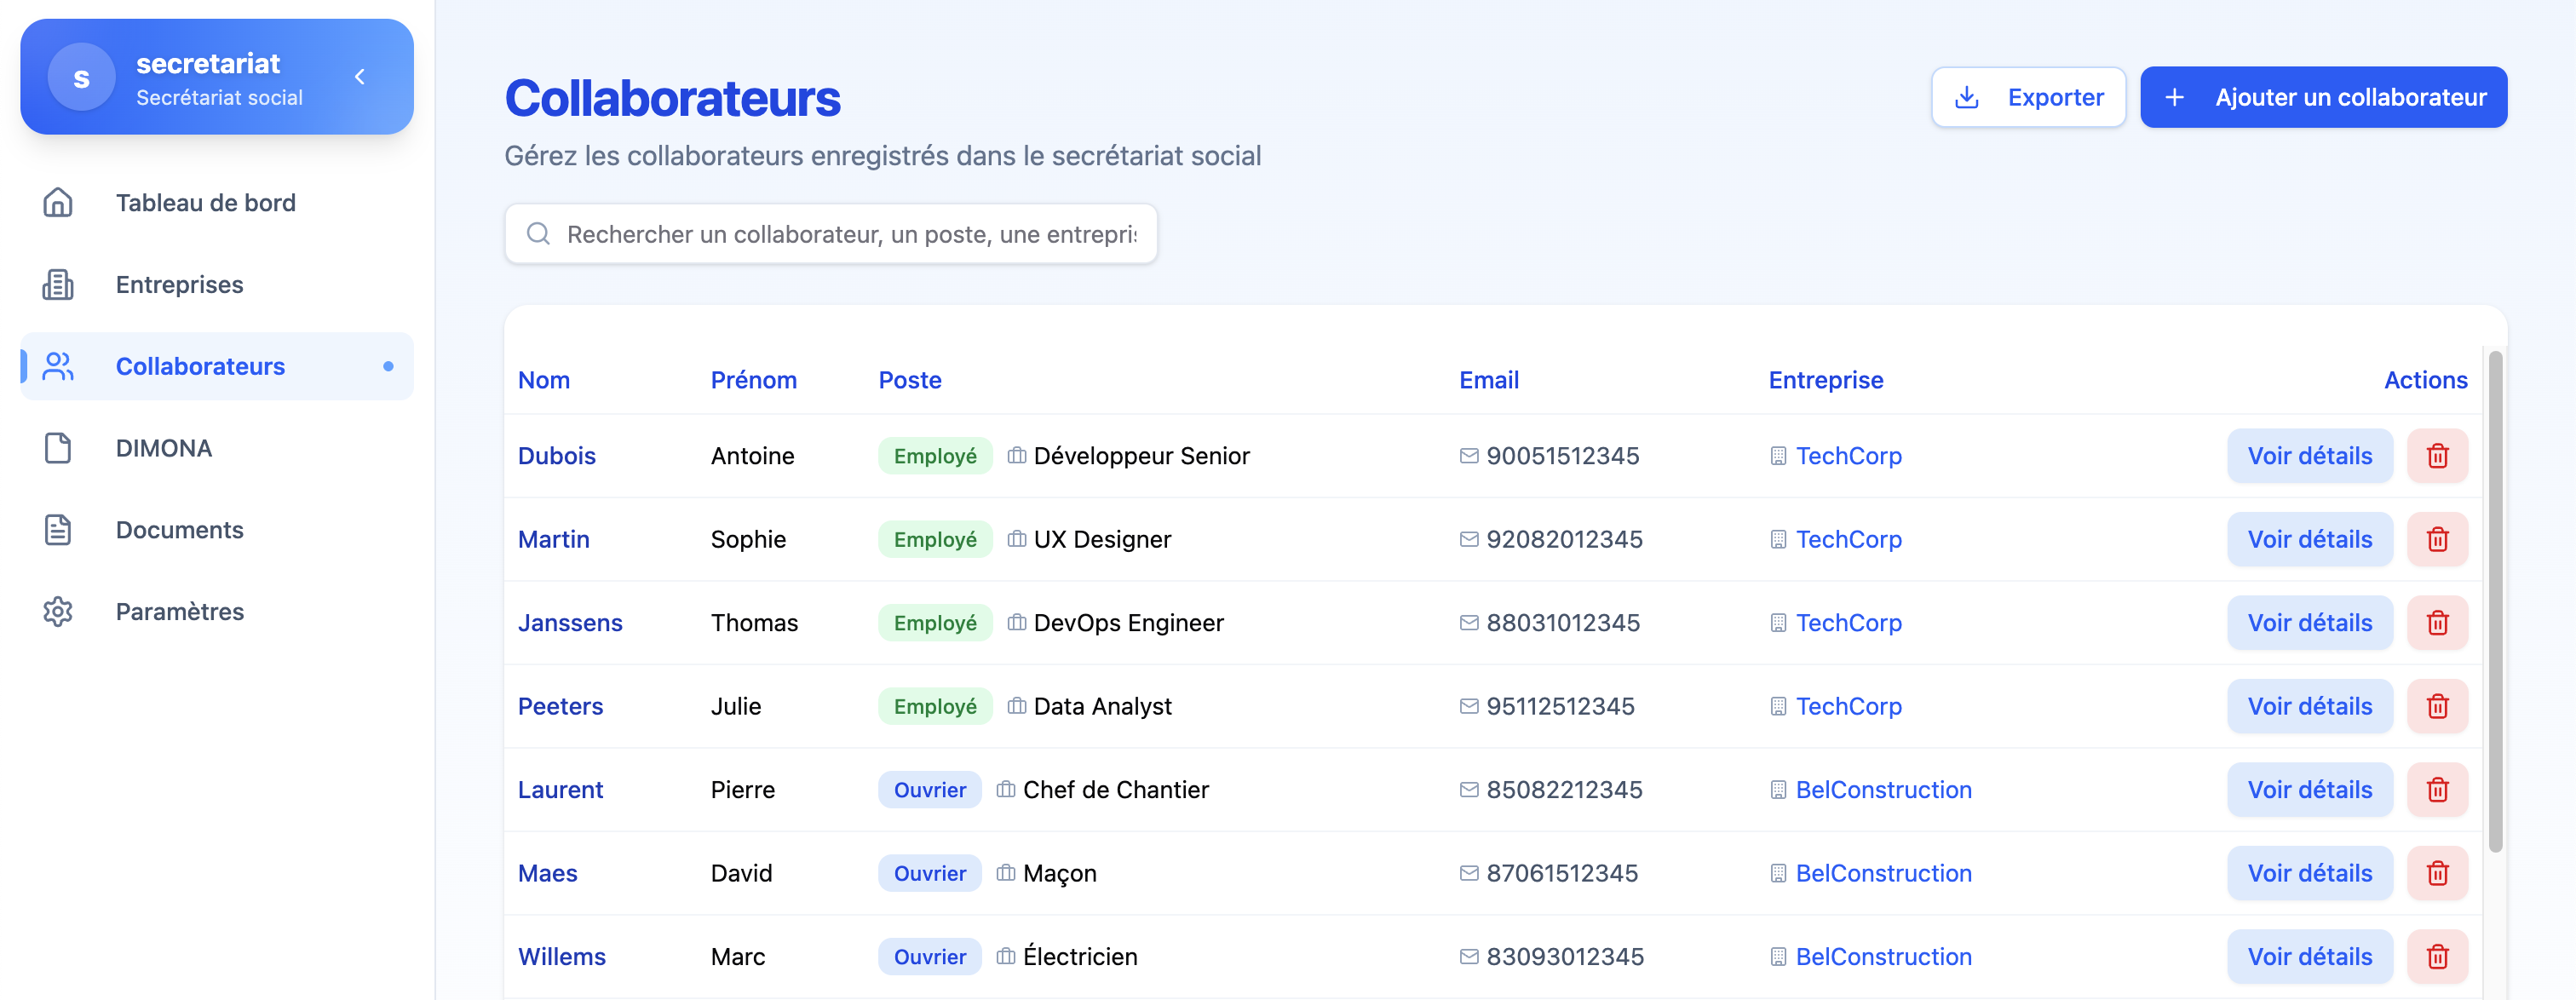
\includegraphics[width=0.7\textwidth]{SecuComPreview.png}
\end{center}

\vspace{2cm}

% Informations sur l'étudiant et le directeur (alignées à droite)
\begin{flushright}
    \large
    \textbf{CHIHI} \textbf{Mehdi}\\
    \vspace{0.3cm}
    \underline{Directeur du suivi :}  \textbf{Mr. Van Oudenhove}\\
    \vspace{0.3cm}
    \textit{Travail de fin d'études présenté en vue de\\
    l'obtention du titre de Bachelier en\\
    \textbf{informatique, orientation développement d'applications}}
\end{flushright}

% Année scolaire (alignée à gauche, tout en bas)
\begin{flushleft}
    \large
    \textbf{Année scolaire} : 2024 - 2025
\end{flushleft}



% Remerciements
% Page de remerciements
\chapter*{\centerline{Remerciements}}
\addcontentsline{toc}{chapter}{Remerciements}

\noindent Au terme de ce parcours académique, je tiens à exprimer ma sincère reconnaissance envers toutes les personnes qui ont contribué, directement ou indirectement, à la réalisation de ce Travail de Fin d'Études.

\vspace{0.5cm}
\noindent Mes remerciements s'adressent tout particulièrement à \textbf{Monsieur Didier Van Oudenhove}, promoteur de ce TFE, pour sa disponibilité constante, ses conseils judicieux et son soutien indéfectible tout au long de ce projet. Sa rigueur intellectuelle et sa vision claire m'ont permis de maintenir le cap sur l'essentiel et d'éviter de me disperser parmi une multitude de fonctionnalités et de me laisser submerger par tous ceux-là.

\vspace{0.5cm}
\noindent J'exprime également ma gratitude envers l'équipe de \textbf{Sodabel}, et spécialement à son dirigeant, \textbf{Monsieur Imad Bazarouji}. Leur précieuse collaboration, le temps qu'ils m'ont accordé et les informations qu'ils ont partagées ont été essentiels dans le développement d'une solution parfaitement adaptée à leurs besoins réels.

\vspace{0.5cm}
\noindent Ma reconnaissance s'étend à l'ensemble du corps professoral de l'\textbf{ISFCE} pour la qualité exceptionnelle de leur enseignement et leur dévouement à former la prochaine génération de développeurs, d'analystes et de professionnels en informatique. Leur expertise et leur passion ont constitué une source d'inspiration permanente.

\vspace{0.5cm}
\noindent Enfin, j'adresse mes remerciements les plus chaleureux à ma famille et mes amis pour leur soutien sans faille, leurs encouragements constants et leur patience remarquable tout au long de mes études. Leur présence bienveillante et leur compréhension ont été fondamentales face aux défis qu'imposait ce rythme intense, alliant cours du soir, activité professionnelle et vie de famille.

\vspace{1cm}
\begin{flushright}
\textit{Avec toute ma reconnaissance,}\\
\vspace{0.3cm}
\end{flushright}

\newpage


% Table des matières
\tableofcontents
\newpage

% Liste des figures
\listoffigures
\newpage

% Liste des tableaux
\listoftables
\newpage

% Introduction
\chapter*{Introduction}
\addcontentsline{toc}{chapter}{Introduction}
\markboth{Introduction}{}

À l'ère numérique, la digitalisation des processus administratifs est devenue essentielle pour les entreprises. Les secrétariats sociaux belges font face à des défis importants liés aux réglementations complexes et au traitement des déclarations DIMONA. Malgré cela, de nombreux secrétariats sociaux indépendants utilisent encore des processus manuels, source d'inefficacités et d'erreurs.

\section*{Objectifs du TFE}
\addcontentsline{toc}{section}{Objectifs du TFE}
\markright{Objectifs du TFE}

Ce Travail de Fin d'Études, présenté à l'ISFCE dans le cadre de l'obtention du diplôme de Bachelier en informatique à orientation développement d'applications, vise à concevoir, développer et valider une plateforme de gestion pour secrétariats sociaux, baptisée \textbf{SecuCom}. Cette solution est spécifiquement adaptée aux besoins de Sodabel, un secrétariat social indépendant avec lequel une collaboration étroite a été établie tout au long du projet.

\vspace{0.5cm}

\begin{tcolorbox}[
  title={\textbf{SecuCom}},
  colback=blue!5!white,
  colframe=primarycolor,
  fonttitle=\bfseries,
  boxrule=0.5mm,
  arc=2mm,
  left=6mm,
  right=6mm,
  top=6mm,
  bottom=6mm
]\textbf{SecuCom} est une plateforme web sécurisée conçue pour simplifier et optimiser les processus administratifs des secrétariats sociaux indépendants. Elle se concentre sur les fonctionnalités essentielles, évitant la complexité souvent rencontrée dans les solutions existantes sur le marché.
\end{tcolorbox}

\vspace{0.5cm}


\noindent Plus précisément, les objectifs de ce TFE sont de :
\begin{itemize}[leftmargin=*,label=\textcolor{darkgray}{$\bullet$},itemsep=0.3em]
  \item Analyser les processus internes de Sodabel concernant la gestion des entreprises clientes, de leurs employés et des déclarations DIMONA
  \item Concevoir une architecture backend robuste et sécurisée répondant aux besoins spécifiques identifiés
  \item Implémenter les fonctionnalités clés permettant de fluidifier les processus d'encodage et de gestion
  \item Valider la solution à travers des tests fonctionnels et de sécurité
  \item Fournir un premier jet d'une solution qui pourra être développée davantage dans un cadre professionnel futur
\end{itemize}

\noindent L'ambition de ce projet dépasse le simple cadre académique. Il s'agit de proposer une solution réellement opérationnelle qui pourra être déployée et améliorée progressivement pour répondre aux besoins concrets d'un secrétariat social en activité, avec une perspective d'évolution à long terme.


\section*{Méthodologie}
\addcontentsline{toc}{section}{Méthodologie}
\markright{Méthodologie}

\noindent Pour atteindre ces objectifs, ce travail s'articule autour de quatre étapes principales, organisées selon une approche méthodique et rigoureuse.

\begin{itemize}[leftmargin=*,label=\textcolor{darkgray}{$\bullet$},itemsep=0.3em]
  \item \textbf{Analyse des besoins} : Entretiens avec les responsables de Sodabel pour identifier les points de friction dans les processus actuels (WhatsApp, email) et leurs limitations.

  \item \textbf{Conception} : Élaboration des spécifications fonctionnelles et techniques avec modélisation UML, en tenant compte des contraintes du projet.

  \item \textbf{Implémentation} : Développement backend suivant les bonnes pratiques, avec focus sur la sécurité des données et la séparation des espaces clients.

  \item \textbf{Validation} : Tests des fonctionnalités pour garantir que la solution répond aux problématiques identifiées.
\end{itemize}

\begin{note}
Une approche itérative a été privilégiée tout au long du projet, permettant des retours réguliers vers les phases précédentes pour affiner la solution en fonction des retours utilisateurs et des contraintes techniques identifiées en cours de développement. Cette flexibilité méthodologique a permis d'adapter la solution aux besoins réels du terrain.
\end{note}

\section*{Structure du document}
\addcontentsline{toc}{section}{Structure du document}
\markright{Structure du document}

Ce TFE suit une progression logique depuis l'analyse initiale jusqu'à l'évaluation finale, structurée comme suit :

\begin{itemize}[leftmargin=*,label=\textcolor{darkgray}{$\bullet$},itemsep=0.3em]
  \item \textbf{Contexte} : Présentation de l'environnement des secrétariats sociaux en Belgique et des problématiques spécifiques de Sodabel.
  
  \item \textbf{Description du sujet} : Exposition de SecuCom, ses objectifs et son fonctionnement, avec accent sur sa simplicité d'utilisation.
  
  \item \textbf{Analyse de l'existant} : Comparaison avec les solutions du marché et positionnement de SecuCom comme alternative ciblée.
  
  \item \textbf{Exigences, besoins et Analyse} : Identification des besoins et leur traduction en architecture système via des diagrammes UML.
  
  \item \textbf{Conception et Développement} : Présentation des choix architecturaux et de l'implémentation des fonctionnalités principales.
  
  \item \textbf{Aspects financiers et Conclusion} : Évaluation économique du projet et perspectives d'évolution future.
\end{itemize}


% Contexte
\chapter{Contexte}

\section{Description du secrétariat social}

Sodabel est une Société à Responsabilité Limitée (SRL) créée le 29 juillet 2020, située Avenue Frans van Kalken 9 à Anderlecht (1070). Cette jeune entreprise, identifiée sous le numéro BE 0751.606.280, est spécialisée dans les activités de service de bureau et de soutien administratif, avec un focus particulier sur les services de secrétariat social.

Malgré sa taille modeste (classée comme micro-entreprise avec 0 équivalent temps plein déclaré), Sodabel offre une gamme complète de services essentiels aux entreprises et indépendants. Ses principales activités comprennent la génération de documents administratifs et sociaux tels que les contrats de travail, les formulaires C4 (documents de fin de contrat), et les fiches de paie. Cette offre de services est complétée par une collaboration étroite avec Fiscobel, une autre entreprise appartenant au même gérant, qui fournit des services comptables complémentaires, créant ainsi un écosystème de support administratif complet pour les clients.

La clientèle de Sodabel est principalement composée d'indépendants et de petites entreprises issues de secteurs variés, avec une forte représentation dans les domaines du transport (taxis), de la restauration et de la construction. Cette spécialisation dans l'accompagnement des petites structures entrepreneuriales répond à un besoin spécifique du marché belge, où les démarches administratives liées à l'emploi peuvent représenter un défi considérable pour les entrepreneurs qui se concentrent sur leur cœur de métier.

\section{Problématique et besoins}

Malgré son expertise dans le domaine du secrétariat social, Sodabel fait face à plusieurs défis opérationnels liés à ses processus actuels, majoritairement manuels. L'absence d'un système informatique dédié engendre des inefficacités et des risques qui impactent tant la qualité du service que la satisfaction client.

Le principal problème identifié concerne la saisie manuelle des données lors de la déclaration des collaborateurs. Ce processus, qu'il soit réalisé en personne au secrétariat ou à distance via des communications par email ou WhatsApp, est particulièrement sujet aux erreurs. Une simple faute de frappe ou une mauvaise interprétation des informations transmises peut avoir des conséquences significatives. En effet, les erreurs dans les déclarations peuvent entraîner des complications légales et administratives tant pour le collaborateur déclaré que pour l'entreprise cliente, pouvant aller jusqu'à des sanctions de la part des organismes de sécurité sociale.

La communication fragmentée entre Sodabel et ses clients constitue un autre point de friction majeur. L'utilisation de canaux multiples et non structurés (visites en personne, emails, messages WhatsApp) pour la transmission d'informations critiques crée un environnement propice aux malentendus et aux oublis. L'absence d'un canal unique et formalisé pour la collecte des données nécessaires aux différentes déclarations sociales complexifie le suivi et augmente le risque d'erreurs.

Enfin, l'absence d'un système de suivi en temps réel des déclarations DIMONA représente une limitation importante. Actuellement, Sodabel ne dispose d'aucun mécanisme proactif pour monitorer le statut des déclarations soumises à l'Office National de Sécurité Sociale (ONSS). Le suivi se fait manuellement ou en réaction aux alertes émises par l'ONSS, ce qui peut retarder la détection et la résolution des problèmes potentiels.

Ces différentes problématiques soulignent un besoin clair de digitalisation et d'automatisation des processus au sein de Sodabel, afin de réduire les risques d'erreurs, d'améliorer l'efficacité opérationnelle et d'offrir un meilleur service à ses clients.

\section{Processus métier}

Pour mieux comprendre les enjeux et les opportunités d'amélioration, il est essentiel d'examiner en détail les principaux processus métier actuellement en place chez Sodabel.

\subsection{Processus de création d'une entreprise cliente}

Lorsqu'une nouvelle entreprise souhaite devenir cliente de Sodabel, le processus actuel est entièrement manuel. L'entreprise doit se présenter physiquement au secrétariat social ou envoyer les informations requises par email ou WhatsApp. Une secrétaire de Sodabel collecte alors manuellement toutes les données nécessaires : informations d'identification de l'entreprise, coordonnées du responsable, secteur d'activité, nombre d'employés prévus, etc. Ces informations sont ensuite saisies dans des fichiers ou des formulaires papier, sans système centralisé permettant un accès facile et sécurisé à ces données.

Ce processus présente plusieurs limitations :
\begin{itemize}
  \item Risque élevé d'erreurs lors de la transcription des données
  \item Temps de traitement important
  \item Difficulté à retrouver et à mettre à jour les informations
  \item Absence de validation automatique des données saisies
\end{itemize}

\subsection{Processus d'ajout d'un collaborateur}

L'ajout d'un nouveau collaborateur pour une entreprise cliente suit un schéma similaire. L'entreprise communique les informations du collaborateur soit en personne, soit par voie électronique (email, WhatsApp). Une secrétaire de Sodabel doit alors saisir manuellement ces données pour préparer les documents nécessaires et effectuer les déclarations obligatoires.

Ce processus est particulièrement critique car les erreurs à ce niveau peuvent avoir des conséquences légales importantes. Une erreur dans la saisie du numéro de registre national, de la date de début de contrat ou du type de contrat peut entraîner des problèmes administratifs significatifs tant pour l'employeur que pour l'employé.

\subsection{Processus de déclaration DIMONA}

La Déclaration Immédiate/Onmiddellijke Aangifte (DIMONA) est une obligation légale en Belgique qui consiste à déclarer immédiatement tout engagement ou fin de relation de travail auprès de l'ONSS. Chez Sodabel, ce processus est actuellement géré de manière réactive.

Lorsqu'une entreprise cliente souhaite déclarer un nouveau collaborateur, elle fournit les informations nécessaires à Sodabel. Une secrétaire saisit alors ces informations dans le système de l'ONSS pour effectuer la déclaration DIMONA. Cependant, il n'existe aucun système interne permettant de suivre en temps réel le statut de ces déclarations. Le suivi se fait manuellement, en vérifiant périodiquement les confirmations reçues de l'ONSS, ou en réaction aux alertes émises par cet organisme en cas de problème.

Cette approche présente plusieurs inconvénients :
\begin{itemize}
  \item Absence de visibilité en temps réel sur le statut des déclarations
  \item Détection tardive des erreurs ou des problèmes
  \item Difficulté à fournir des informations actualisées aux clients
  \item Risque accru de non-conformité avec les obligations légales
\end{itemize}

L'ensemble de ces processus métier, bien que fonctionnels, présente des inefficacités et des risques qui justifient pleinement le développement d'une solution informatique dédiée comme SecuCom. Cette plateforme vise à digitaliser et à automatiser ces processus, réduisant ainsi les risques d'erreurs tout en améliorant l'efficacité opérationnelle et la qualité du service offert par Sodabel à ses clients.


% Description du sujet
\chapter{Description du sujet}

\section{Qu'est-ce que SecuCom ?}

\textbf{SecuCom} est une plateforme de gestion sécurisée spécifiquement conçue pour les secrétariats sociaux et leurs entreprises clientes. Elle se présente sous la forme d'une application web offrant des espaces privés distincts où les différents acteurs peuvent interagir et gérer leurs données administratives de manière fluide et sécurisée.

\begin{figure}[H]
    \centering
    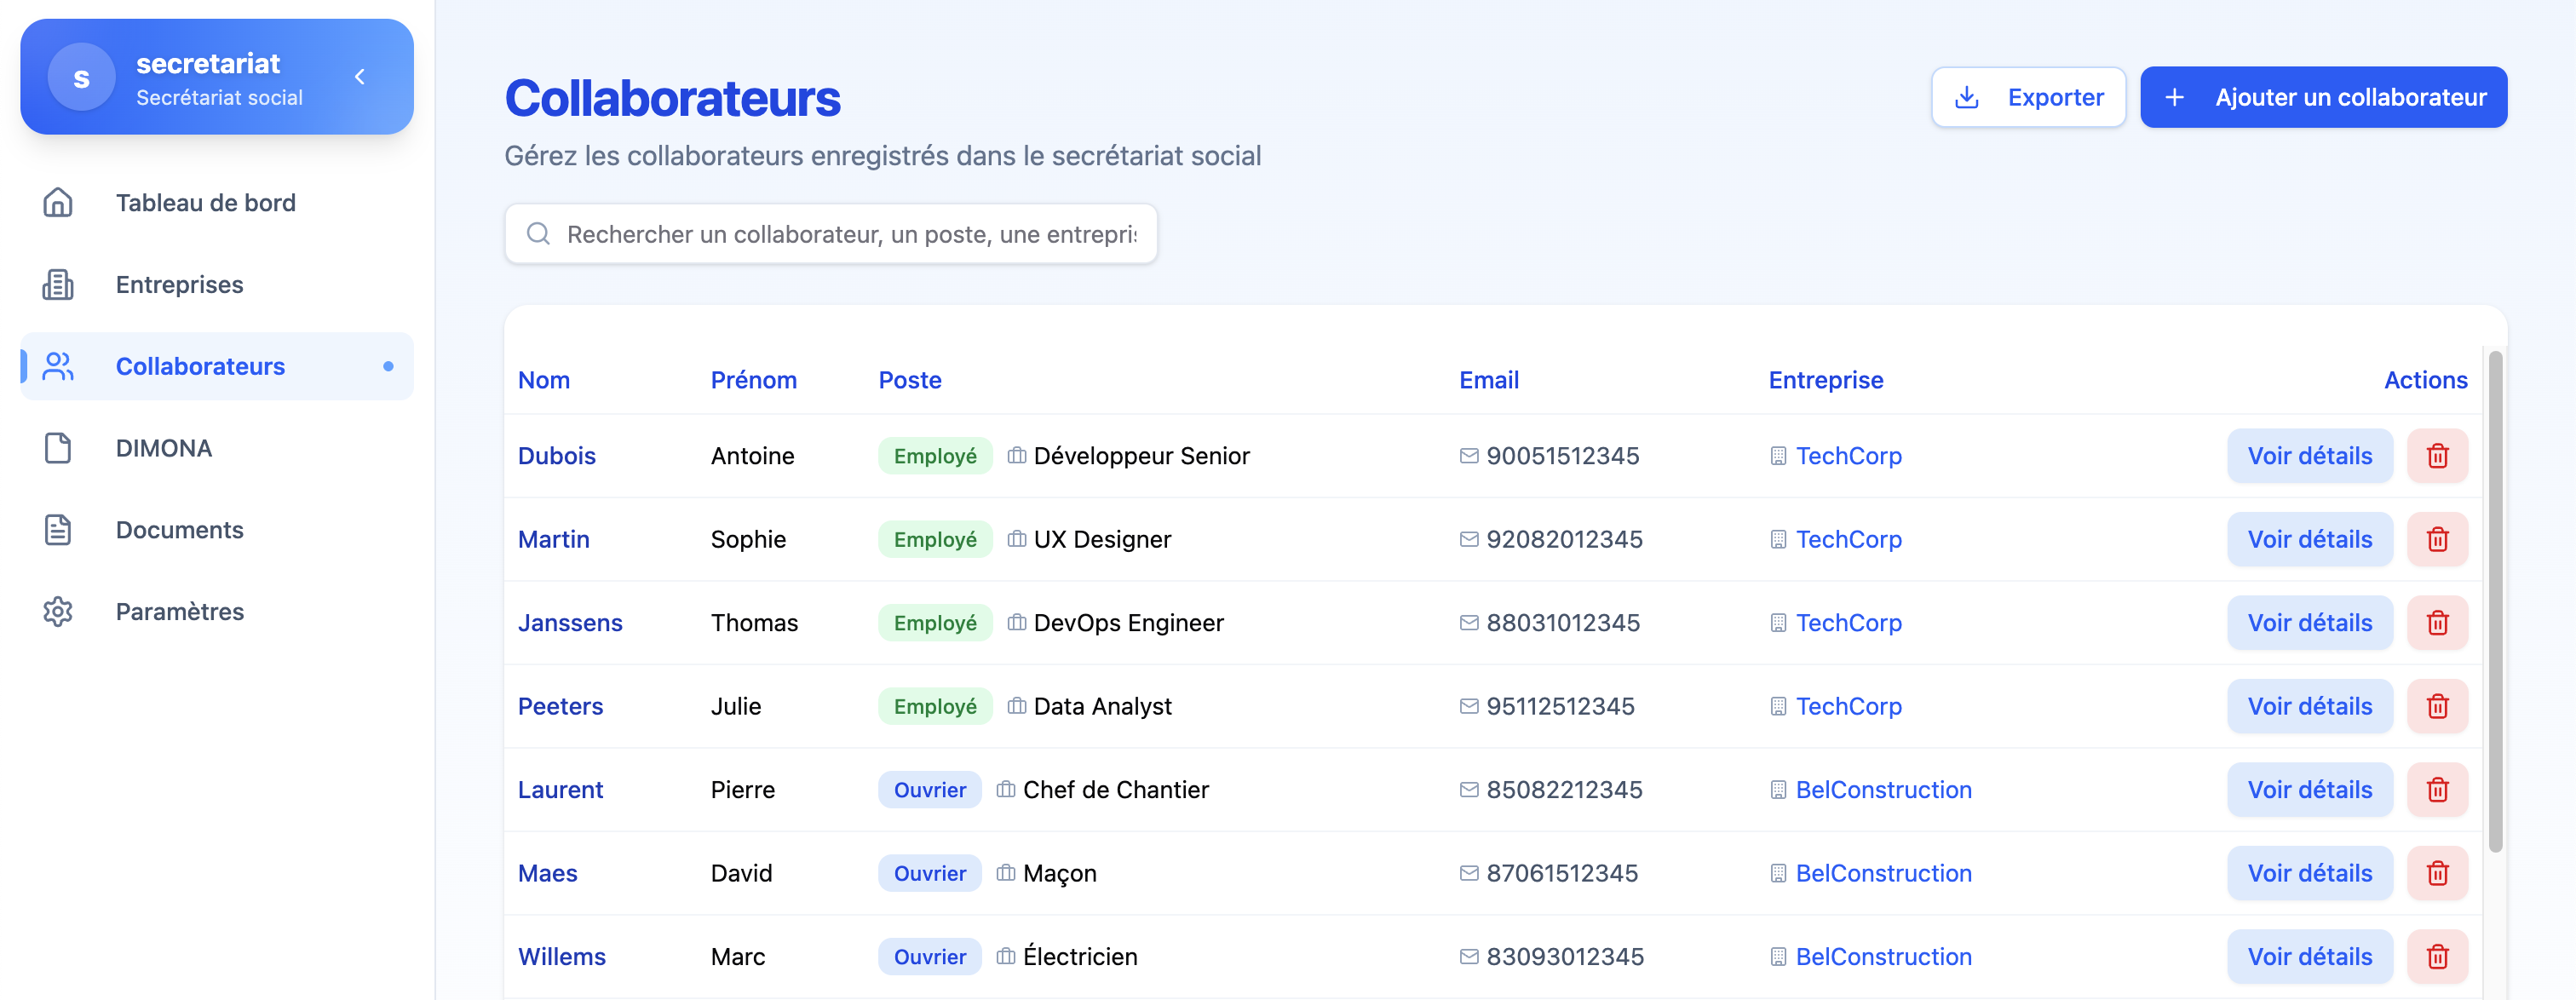
\includegraphics[width=0.9\textwidth]{SecuComPreview.png}
    \caption{Aperçu de l'interface de SecuCom}
    \label{fig:secucomPreview}
\end{figure}

\noindent Au cœur de \textbf{SecuCom} se trouve un système de gestion centralisé permettant la création, la modification et la suppression de trois types d'entités principales :
\begin{itemize}[leftmargin=*,label=\textcolor{darkgray}{$\bullet$},itemsep=0.3em]
  \item Les entreprises clientes du secrétariat social
  \item Les collaborateurs (employés) rattachés à ces entreprises
  \item Les déclarations DIMONA associées à ces collaborateurs
\end{itemize}

\vspace{0.5cm}

\noindent Contrairement aux processus manuels actuels décrits dans la section précédente, \textbf{SecuCom} offre une interface numérique unifiée qui remplace les échanges fragmentés par email et WhatsApp. Cette approche centralisée permet non seulement de réduire les risques d'erreurs lors de la saisie des données, mais aussi de faciliter le suivi et la mise à jour manuelle du statut des déclarations DIMONA, élément crucial pour la conformité légale des entreprises.

\begin{note}
L'interface utilisateur de \textbf{SecuCom} a été conçue avec une philosophie minimaliste, privilégiant la clarté et l'intuitivité. Les fonctionnalités essentielles sont mises en évidence, permettant aux utilisateurs de naviguer efficacement sans formation approfondie. Cette simplicité apparente masque cependant une architecture robuste qui gère de manière transparente les complexités des processus administratifs sous-jacents, tout en s'appuyant sur des validations internes plutôt que sur des intégrations API externes.
\end{note}

\begin{tcolorbox}[
  title={\textbf{Fonctionnalités clés de SecuCom}},
  colback=blue!5!white,
  colframe=primarycolor,
  fonttitle=\bfseries,
  boxrule=0.5mm,
  arc=2mm,
  left=6mm,
  right=6mm,
  top=6mm,
  bottom=6mm
]
\begin{itemize}[leftmargin=*,label=\textcolor{darkgray}{$\bullet$},itemsep=0.3em]
  \item La gestion sécurisée des profils d'entreprises clientes avec toutes leurs informations administratives
  \item L'encodage structuré des données des collaborateurs avec validation interne pour minimiser les erreurs
  \item La création assistée des déclarations DIMONA avec possibilité de mise à jour manuelle de leur statut
  \item Un système de notifications pour alerter les utilisateurs des actions requises ou des problèmes potentiels
  \item Une séparation stricte des accès garantissant la confidentialité des données sensibles
\end{itemize}
\end{tcolorbox}

\vspace{0.5cm}

\noindent \textbf{SecuCom} se distingue par sa focalisation exclusive sur les besoins spécifiques des secrétariats sociaux de petite taille et de leurs clients, offrant ainsi une solution sur mesure là où les plateformes généralistes proposent souvent des fonctionnalités superflues qui complexifient l'expérience utilisateur.

\section{À qui est destiné SecuCom ?}

\textbf{SecuCom} s'adresse principalement à deux catégories d'utilisateurs, chacune avec des besoins et des niveaux d'accès spécifiques :

\subsection{Le personnel du secrétariat social (Sodabel)}

\begin{itemize}[leftmargin=*,label=\textcolor{darkgray}{$\bullet$},itemsep=0.3em]
  \item \textbf{Le personnel du secrétariat} : Les utilisateurs du secrétariat social bénéficient d'un accès complet à toutes les entreprises clientes, leurs collaborateurs et leurs déclarations DIMONA. L'interface leur permet de traiter efficacement les demandes, de vérifier les informations et d'effectuer les déclarations officielles auprès des organismes compétents.
\end{itemize}

\begin{note}
Dans la version actuelle de \textbf{SecuCom}, un seul rôle "secrétariat" est implémenté pour tous les utilisateurs de Sodabel. Une distinction plus fine entre les rôles (comme gérant et secrétaires) pourra être développée ultérieurement selon les besoins spécifiques identifiés lors de l'utilisation du système.
\end{note}

\vspace{0.5cm}

\noindent Pour ces utilisateurs, \textbf{SecuCom} offre une vue d'ensemble de tous les clients, permettant une gestion transversale et efficace des dossiers. L'interface est optimisée pour faciliter le traitement en série des demandes et la gestion simultanée de multiples entreprises clientes.

\subsection{Le personnel administratif des entreprises clientes}

\textbf{Les employés administratifs} désignés par chaque entreprise cliente ont accès à un espace privé limité aux données de leur propre organisation. Ils peuvent :
\begin{itemize}[leftmargin=*,label=\textcolor{darkgray}{$\bullet$},itemsep=0.3em]
  \item Consulter et mettre à jour les informations de leur entreprise
  \item Gérer leurs propres collaborateurs (ajout, modification, suppression)
  \item Initier des demandes de déclaration DIMONA
  \item Suivre l'état d'avancement de leurs déclarations
\end{itemize}

\vspace{0.5cm}

\noindent Pour ces utilisateurs, l'interface est simplifiée et focalisée uniquement sur leurs propres données, éliminant toute distraction ou confusion potentielle. Les actions possibles sont clairement délimitées et guidées pour minimiser les erreurs.

\begin{tcolorbox}[
  title={\textbf{Séparation des accès}},
  colback=blue!5!white,
  colframe=primarycolor,
  fonttitle=\bfseries,
  boxrule=0.5mm,
  arc=2mm,
  left=6mm,
  right=6mm,
  top=6mm,
  bottom=6mm
]
\noindent Cette séparation stricte des accès est un élément fondamental de l'architecture de \textbf{SecuCom} :
\begin{itemize}[leftmargin=*,label=\textcolor{darkgray}{$\bullet$},itemsep=0.3em]
  \item \textbf{Sodabel} peut voir l'ensemble des clients et de leurs données
  \item \textbf{Chaque entreprise} est confinée à son propre périmètre
\end{itemize}

\noindent Cette approche garantit non seulement la confidentialité des données sensibles, mais simplifie également l'expérience utilisateur en ne présentant à chacun que les informations pertinentes pour son rôle.
\end{tcolorbox}

\vspace{0.5cm}

\noindent L'interface épurée et intuitive de \textbf{SecuCom} a été spécifiquement conçue pour s'adapter à des utilisateurs ayant des niveaux variables de compétences informatiques, reconnaissant que dans de nombreuses petites entreprises, les tâches administratives sont souvent gérées par du personnel non spécialisé. Les formulaires incluent des validations intelligentes et des indications contextuelles pour guider les utilisateurs et prévenir les erreurs courantes.

\begin{note}
Les validations en temps réel des formulaires permettent de détecter immédiatement les erreurs potentielles, comme un numéro de registre national mal formaté ou une date de début de contrat incohérente, évitant ainsi des problèmes administratifs ultérieurs.
\end{note}

\vspace{0.5cm}

\noindent En résumé, \textbf{SecuCom} offre une expérience sur mesure pour chaque type d'utilisateur, tout en maintenant une cohérence globale qui facilite la communication et la collaboration entre le secrétariat social et ses clients.


% Analyse de l'existant
\chapter{Analyse de l'existant}

\section{Démarche d'analyse de l'existant}

\noindent Pour évaluer le positionnement de \textbf{SecuCom} dans le paysage des solutions destinées aux secrétariats sociaux, une analyse approfondie des plateformes existantes a été menée. Cette démarche s'est articulée autour de plusieurs axes :

\begin{itemize}[leftmargin=*,label=\textcolor{darkgray}{$\bullet$},itemsep=0.3em]
  \item Étude documentaire des solutions leaders du marché belge, notamment via leurs sites officiels, leurs documentations techniques et leurs présentations commerciales
  \item Entretiens avec des utilisateurs actuels de ces plateformes au sein de différents secrétariats sociaux
  \item Analyse comparative des fonctionnalités, des modèles tarifaires et des approches d'intégration
  \item Identification des forces et faiblesses de chaque solution par rapport aux besoins spécifiques des petits secrétariats sociaux comme Sodabel
\end{itemize}

\vspace{0.5cm}

\noindent Cette méthodologie a permis d'établir une cartographie précise de l'offre existante et d'identifier les opportunités pour une solution comme \textbf{SecuCom}. Deux acteurs majeurs ont particulièrement retenu notre attention en raison de leur prédominance sur le marché belge : EasyPay et Liantis.

\begin{note}
L'analyse comparative s'est concentrée sur les fonctionnalités pertinentes pour les petits secrétariats sociaux, en accordant une attention particulière à la facilité d'utilisation, au coût et à l'adéquation avec les processus métier spécifiques de structures comme Sodabel.
\end{note}

\section{Analyse comparée des solutions}

\subsection{EasyPay}

\begin{figure}[H]
    \centering
    
\includegraphics[width=0.5\textwidth]{easyPayLogo.jpeg}
    \caption{Logo d'EasyPay Group \cite{easypay}}
    \label{fig:easyPayLogo}
\end{figure}

\noindent EasyPay Group se positionne comme un acteur incontournable dans le domaine des services de secrétariat social et de gestion des ressources humaines en Belgique. Cette plateforme propose une suite complète d'outils couvrant l'ensemble des besoins administratifs et RH d'une entreprise :

\begin{itemize}[leftmargin=*,label=\textcolor{darkgray}{$\bullet$},itemsep=0.3em]
  \item Gestion complète de la paie et des déclarations sociales
  \item Administration du personnel de A à Z
  \item Gestion des temps et des plannings
  \item Recrutement et sélection
  \item Développement des compétences et formations
  \item Outils de reporting et tableaux de bord RH
  \item Solutions de digitalisation des processus RH
\end{itemize}

\vspace{0.5cm}

\noindent L'écosystème EasyPay se caractérise par sa richesse fonctionnelle et son approche intégrée. Chaque module communique avec les autres, offrant une expérience utilisateur cohérente et des flux de données optimisés. Cette intégration poussée représente un avantage considérable pour les grandes structures ayant des besoins diversifiés.

\begin{figure}[H]
    \centering
    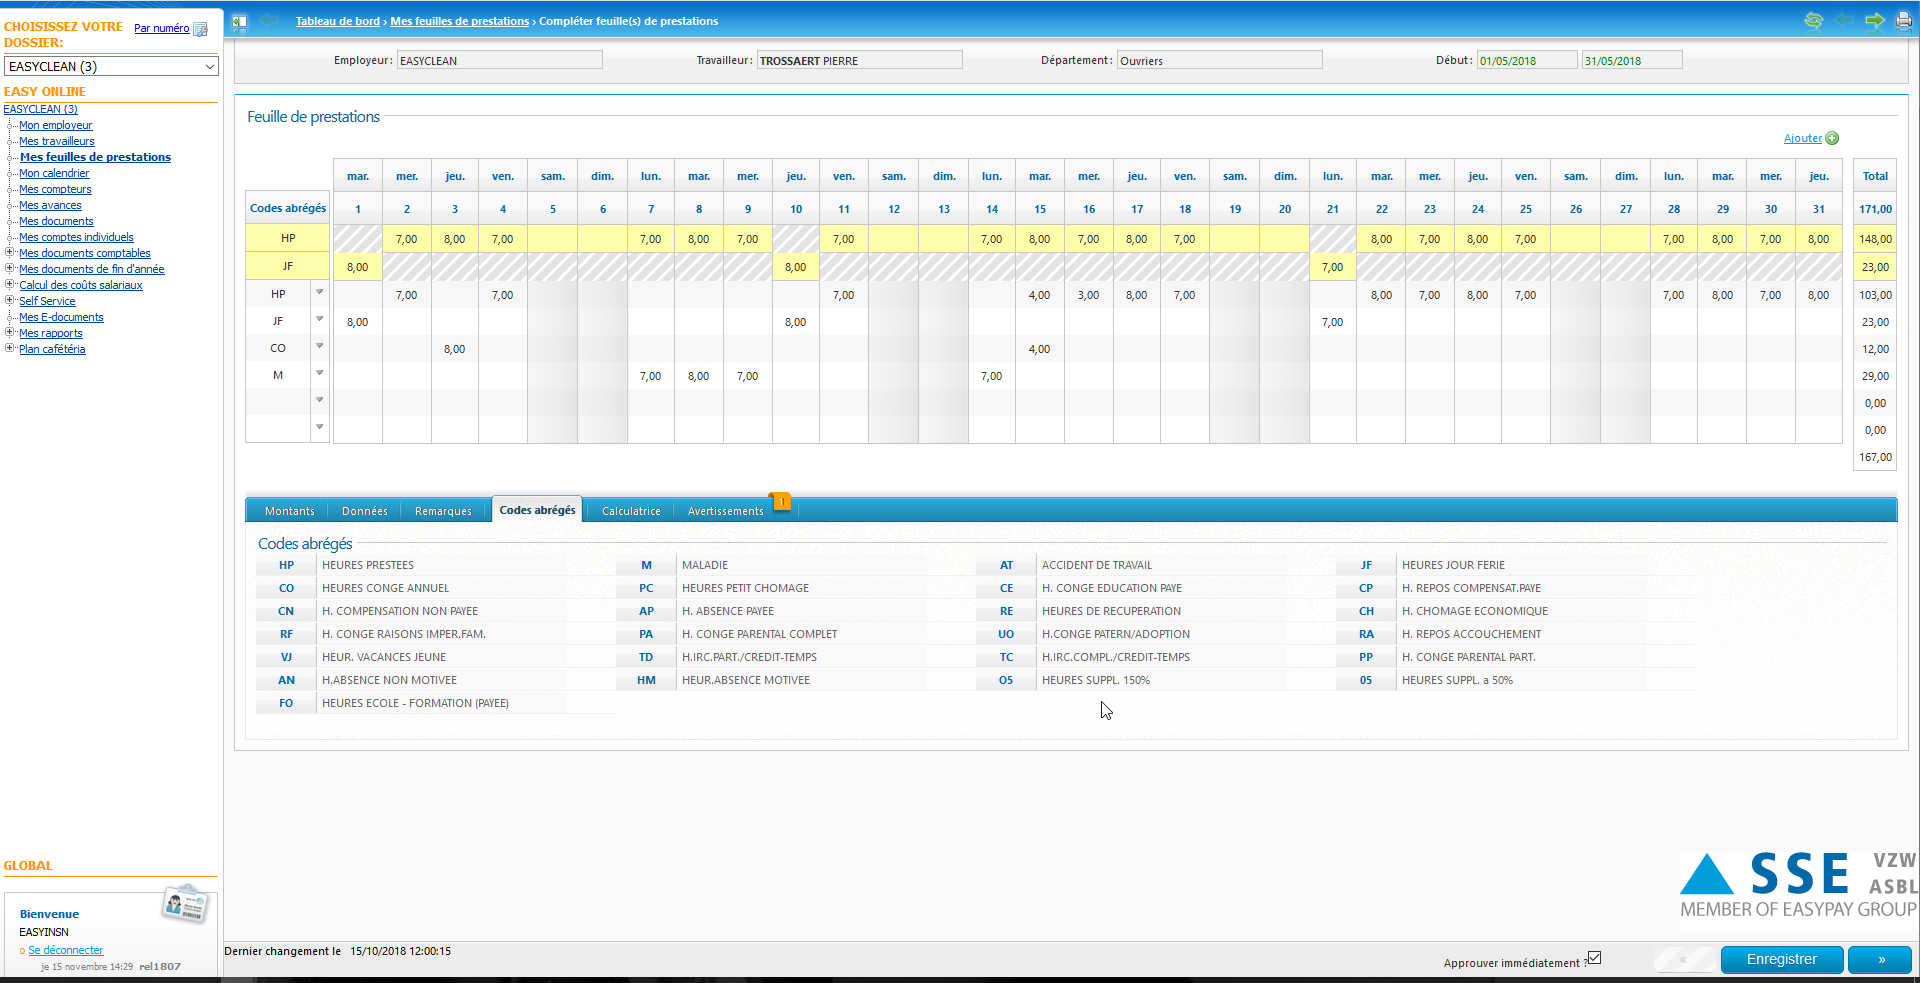
\includegraphics[width=0.9\textwidth]{easyPayScreenshot.png}
    \caption{Capture d'écran de l'interface d'EasyPay \cite{easypay}}
    \label{fig:easyPayScreenshot}
\end{figure}

\begin{tcolorbox}[
  title={\textbf{Limites d'EasyPay pour les petites structures}},
  colback=blue!5!white,
  colframe=primarycolor,
  fonttitle=\bfseries,
  boxrule=0.5mm,
  arc=2mm,
  left=6mm,
  right=6mm,
  top=6mm,
  bottom=6mm
]
\noindent Cette exhaustivité constitue également le principal inconvénient d'EasyPay pour les petites structures comme Sodabel. La plateforme s'avère souvent :
\begin{itemize}[leftmargin=*,label=\textcolor{darkgray}{$\bullet$},itemsep=0.3em]
  \item Excessivement complexe à appréhender et à maîtriser
  \item Coûteuse à déployer et à maintenir
  \item Surdimensionnée par rapport aux besoins réels d'un petit secrétariat social
  \item Rigide dans ses processus, laissant peu de place à la personnalisation fine
\end{itemize}
\end{tcolorbox}

\vspace{0.5cm}

\noindent En outre, bien qu'EasyPay propose des fonctionnalités de gestion des entreprises clientes et de leurs collaborateurs, son interface n'est pas spécifiquement optimisée pour les flux de travail propres aux petits secrétariats sociaux indépendants, qui nécessitent souvent plus d'agilité et de flexibilité dans leurs processus.

\subsection{Liantis}

\begin{figure}[H]
    \centering
    
\includegraphics[width=0.5\textwidth]{liantisLogo.png}
    \caption{Logo de Liantis \cite{liantis}}
    \label{fig:liantisLogo}
\end{figure}

\noindent Liantis représente un autre mastodonte du secteur, né de la fusion de plusieurs acteurs historiques du marché belge. Cette plateforme se distingue par son approche "guichet unique" pour les entrepreneurs et les employeurs, couvrant un spectre extrêmement large de services :

\begin{itemize}[leftmargin=*,label=\textcolor{darkgray}{$\bullet$},itemsep=0.3em]
  \item Secrétariat social complet
  \item Assurances sociales pour indépendants
  \item Médecine du travail et prévention
  \item Allocations familiales
  \item Assurances diverses (accidents du travail, revenu garanti, etc.)
  \item Conseil juridique et accompagnement
  \item Formation et développement
\end{itemize}

\vspace{0.5cm}

\noindent La force de Liantis réside dans cette approche holistique qui permet à une entreprise de gérer l'ensemble de ses obligations sociales et administratives via un seul partenaire. La plateforme offre également des outils numériques modernes et une présence physique étendue à travers la Belgique.

\begin{figure}[H]
    \centering
    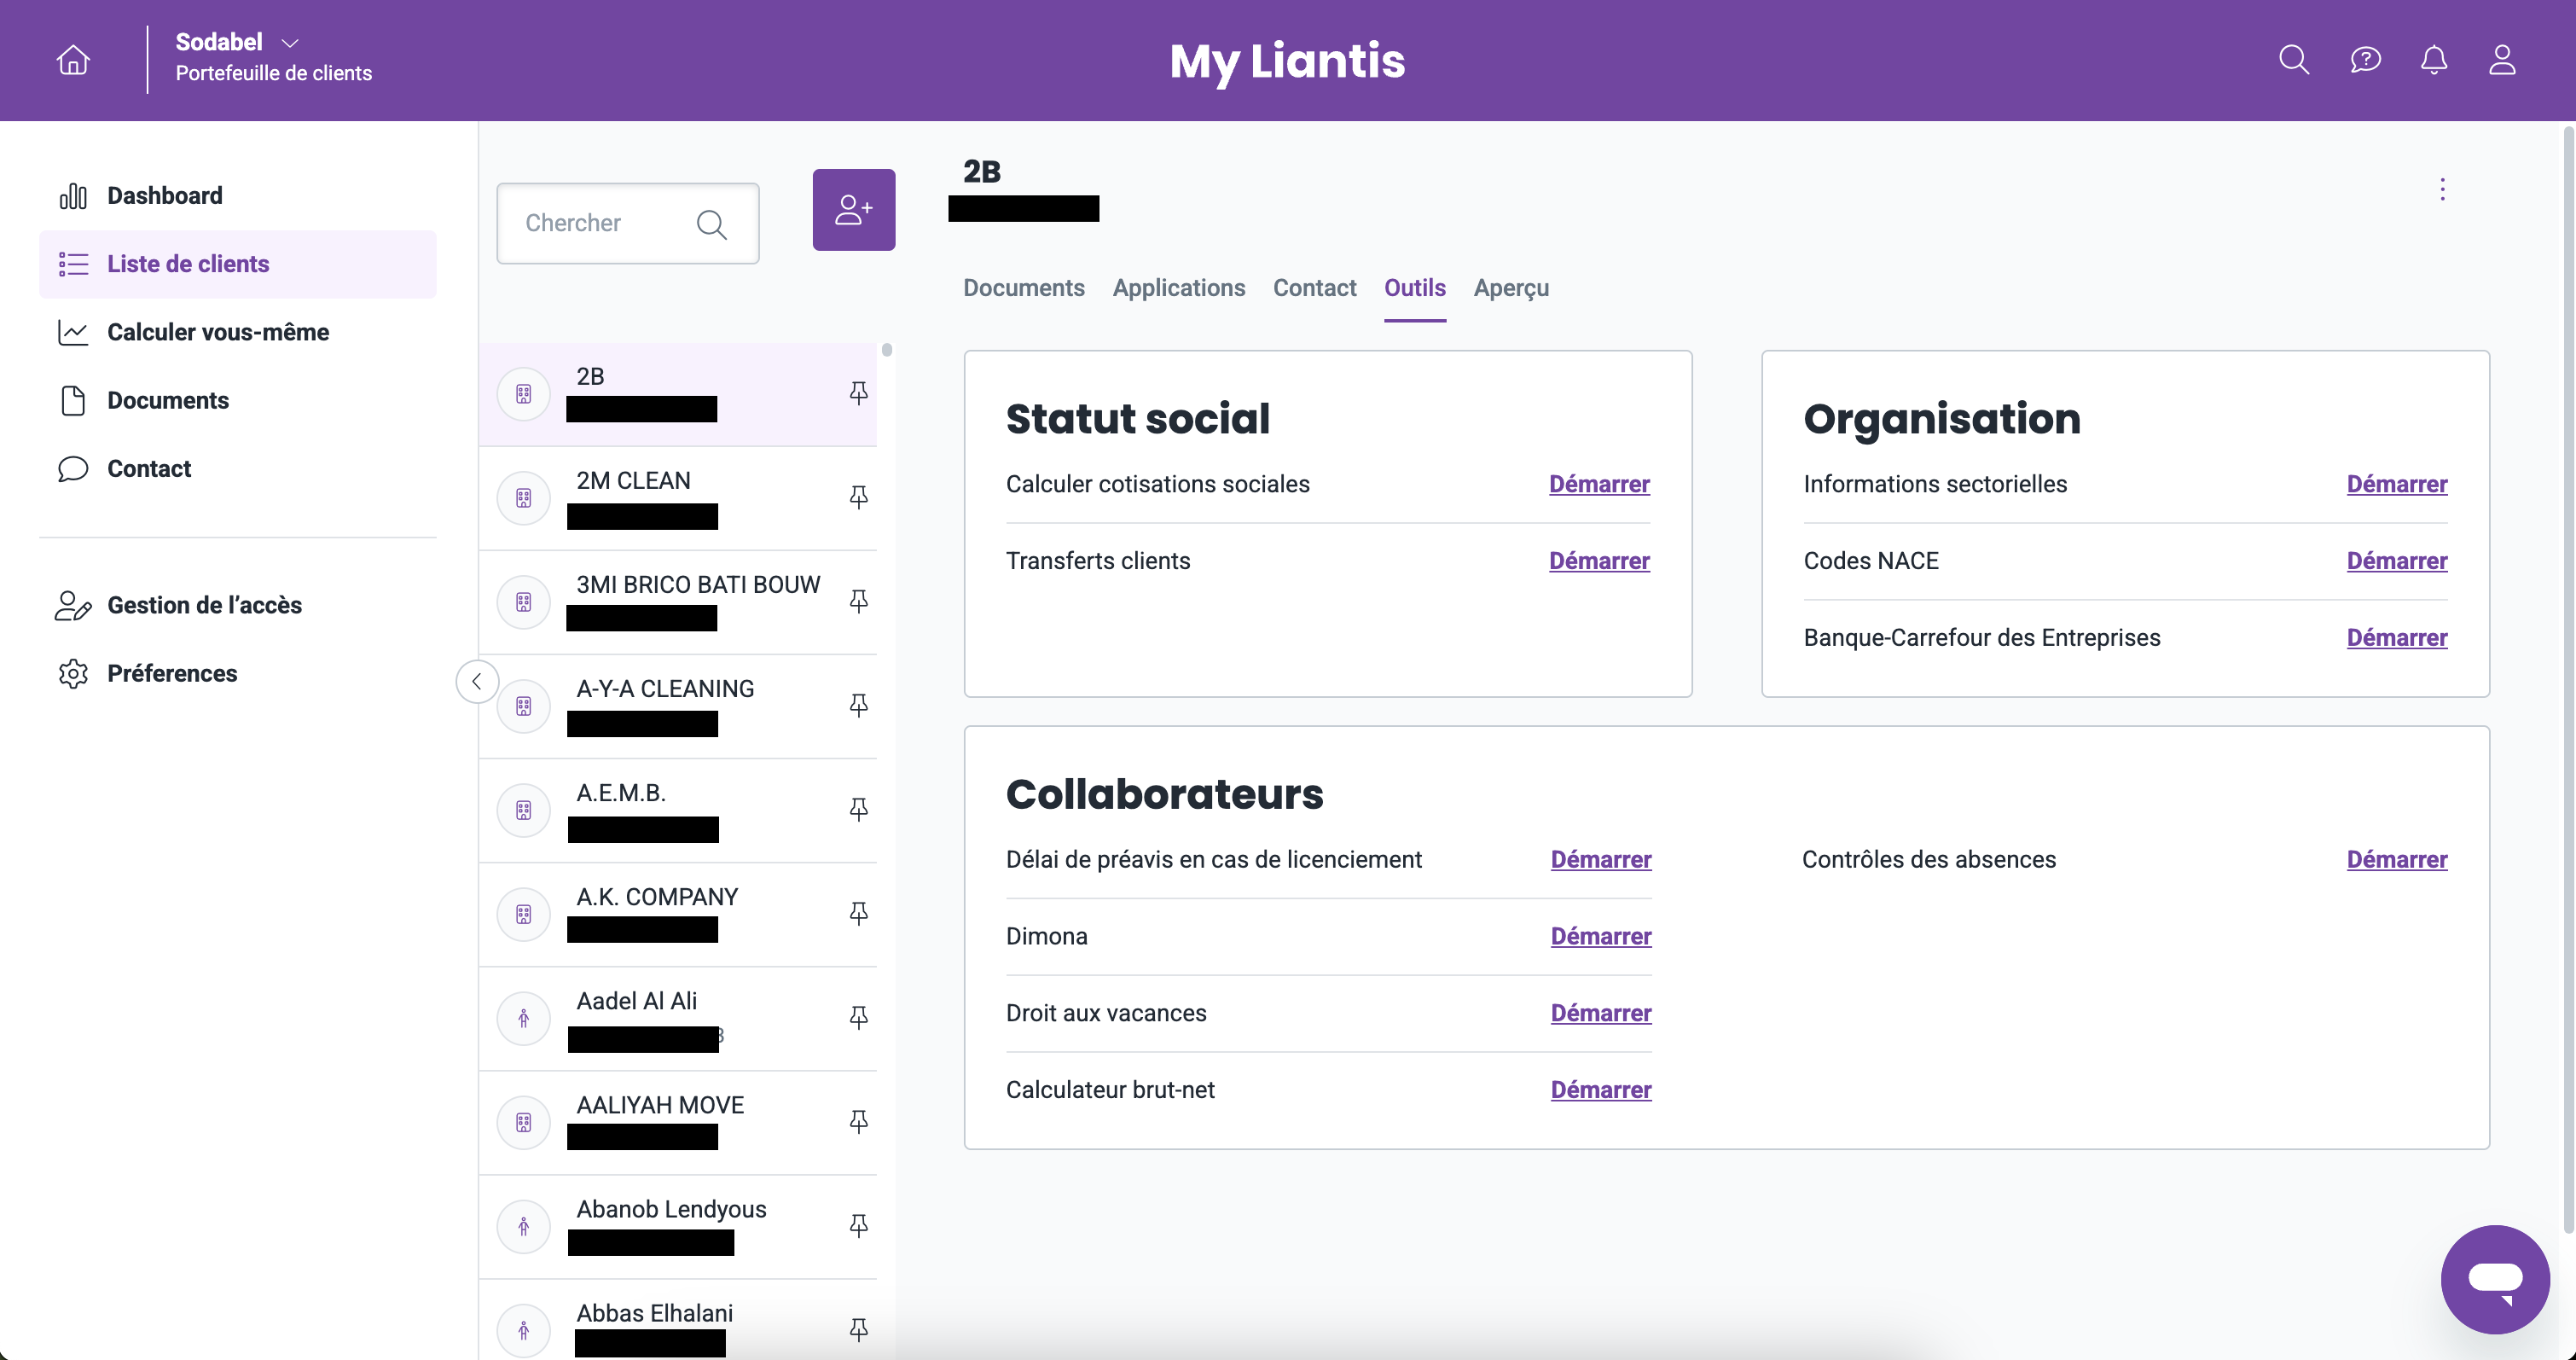
\includegraphics[width=0.9\textwidth]{liantisScreenshot.png}
    \caption{Capture d'écran de l'interface de Liantis \cite{liantis}}
    \label{fig:liantisScreenshot}
\end{figure}

\begin{tcolorbox}[
  title={\textbf{Contraintes de Liantis pour les petites structures}},
  colback=blue!5!white,
  colframe=primarycolor,
  fonttitle=\bfseries,
  boxrule=0.5mm,
  arc=2mm,
  left=6mm,
  right=6mm,
  top=6mm,
  bottom=6mm
]
\noindent Toutefois, comme pour EasyPay, cette exhaustivité s'accompagne de contraintes significatives :
\begin{itemize}[leftmargin=*,label=\textcolor{darkgray}{$\bullet$},itemsep=0.3em]
  \item Une structure tarifaire complexe et souvent onéreuse pour les petites structures
  \item Une certaine lourdeur administrative inhérente à la taille de l'organisation
  \item Des processus standardisés qui peuvent manquer de souplesse
  \item Une interface utilisateur qui, bien que moderne, doit accommoder tant de fonctionnalités qu'elle en devient parfois confuse
\end{itemize}
\end{tcolorbox}

\vspace{0.5cm}

\noindent Par ailleurs, la spécialisation de Liantis dans tant de domaines différents dilue inévitablement son focus sur les besoins spécifiques des petits secrétariats sociaux en matière de gestion des entreprises clientes et de leurs collaborateurs.

\section{SecuCom face à l'existant}

\noindent \textbf{SecuCom} se distingue fondamentalement d'EasyPay et Liantis par son approche ciblée et minimaliste. Là où ces mastodontes tentent de couvrir l'intégralité du spectre des besoins administratifs et sociaux, \textbf{SecuCom} se concentre exclusivement sur l'optimisation des processus de gestion des entreprises clientes, de leurs collaborateurs et des déclarations DIMONA.

\begin{note}
Cette spécialisation délibérée constitue la principale force de \textbf{SecuCom} et répond à un besoin précis que les solutions généralistes, malgré leur richesse fonctionnelle, peinent à satisfaire efficacement. \textbf{SecuCom} n'a jamais eu l'ambition de rivaliser frontalement avec ces géants du secteur, mais plutôt de combler une niche spécifique avec une solution sur mesure.
\end{note}

\begin{tcolorbox}[
  title={\textbf{Avantages distinctifs de SecuCom}},
  colback=blue!5!white,
  colframe=primarycolor,
  fonttitle=\bfseries,
  boxrule=0.5mm,
  arc=2mm,
  left=6mm,
  right=6mm,
  top=6mm,
  bottom=6mm
]
\noindent Les avantages distinctifs de \textbf{SecuCom} par rapport à ces plateformes généralistes sont multiples :

\begin{itemize}[leftmargin=*,label=\textcolor{darkgray}{$\bullet$},itemsep=0.3em]
  \item \textbf{Simplicité et intuitivité} : Interface épurée, focalisée uniquement sur les fonctionnalités essentielles, sans la surcharge cognitive des plateformes tout-en-un.
  \item \textbf{Coût optimisé} : Structure tarifaire simple et adaptée aux petites structures, sans modules superflus à financer.
  \item \textbf{Flexibilité maximale} : Capacité d'adaptation rapide aux processus spécifiques de chaque secrétariat social, contrairement aux workflows rigides des grandes plateformes.
  \item \textbf{Prise en main immédiate} : Courbe d'apprentissage réduite, permettant une adoption rapide sans formation extensive.
  \item \textbf{Focus sur l'essentiel} : Concentration des ressources de développement sur l'optimisation des fonctionnalités réellement utilisées au quotidien.
\end{itemize}
\end{tcolorbox}

\vspace{0.5cm}

\noindent Le tableau comparatif ci-dessous met en évidence le positionnement de \textbf{SecuCom} face à EasyPay et Liantis sur plusieurs critères clés :

\begin{table}[H]
\caption{Comparaison des solutions pour secrétariats sociaux}
\label{tab:comparaison-solutions}

\makebox[\textwidth][c]{%
\renewcommand{\arraystretch}{1.3}
\begin{tabular}{p{3.2cm}p{4.2cm}p{4.2cm}p{4.2cm}}
\toprule
\rowcolor{darkgray} \textcolor{white}{\textbf{Critère}} & \textcolor{white}{\textbf{SecuCom}} & \textcolor{white}{\textbf{EasyPay}} & \textcolor{white}{\textbf{Liantis}} \\
\midrule

\textbf{Étendue fonc\-tionnelle} & 
\textbf{Ciblée} \newline
\small{Gestion entreprises, collaborateurs,\ DIMONA} & 
\textbf{Complète} \newline
\small{Paie, RH, temps, recrutement, etc.} & 
\textbf{Très large} \newline
\small{Social, assurances, médecine du travail, etc.} \\
\midrule

\textbf{Complexité d'utilisation} & 
\textcolor{green!70!black}{\small\textbf{Faible}} \newline
\small{Interface minimaliste} & 
\textcolor{orange!70!black}{\small\textbf{Élevée}} \newline
\small{Nombreux modules interconnectés} & 
\textcolor{red!70!black}{\small\textbf{Très élevée}} \newline
\small{Écosystème complet} \\
\midrule

\textbf{Coût relatif} & 
\textcolor{green!70!black}{\small\textbf{Optimisé}} \newline
\small{Adapté aux petites structures} & 
\textcolor{orange!70!black}{\small\textbf{Élevé}} \newline
\small{Licence + modules} & 
\textcolor{red!70!black}{\small\textbf{Très élevé}} \newline
\small{Services multiples} \\
\midrule

\textbf{Personnalisation} & 
\textcolor{green!70!black}{\small\textbf{Élevée}} \newline
\small{Adaptable aux processus spécifiques} & 
\textcolor{orange!70!black}{\small\textbf{Moyenne}} \newline
\small{Paramétrage dans cadre défini} & 
\textcolor{red!70!black}{\small\textbf{Faible}} \newline
\small{Processus standardisés} \\
\midrule

\textbf{Temps de prise en main} & 
\textcolor{green!70!black}{\small\textbf{Court}} \newline
\small{Quelques heures} & 
\textcolor{orange!70!black}{\small\textbf{Long}} \newline
\small{Plusieurs jours} & 
\textcolor{red!70!black}{\small\textbf{Très long}} \newline
\small{Plusieurs semaines} \\
\midrule

\textbf{Cible principale} & 
\textbf{Petits secrétariats sociaux} \newline
\small{Structures indépendantes} & 
\textbf{Moyennes et grandes entreprises} \newline
\small{Besoins diversifiés} & 
\textbf{Tout type d'entreprise} \newline
\small{Et d'indépendant} \\
\bottomrule
\end{tabular}%
}
\end{table}

\vspace{0.5cm}

\noindent En définitive, \textbf{SecuCom} ne cherche pas à remplacer des plateformes comme EasyPay ou Liantis, mais à offrir une alternative ciblée pour les secrétariats sociaux qui privilégient la simplicité, l'efficacité et la spécialisation. Dans un marché dominé par des solutions toujours plus complètes mais aussi plus complexes, \textbf{SecuCom} répond à un besoin croissant de retour à l'essentiel et d'outils parfaitement adaptés à des cas d'usage spécifiques.

\begin{note}
Cette approche s'inscrit dans une tendance plus large observée dans de nombreux secteurs technologiques : face aux suites logicielles massives qui tentent de tout faire, émergent des solutions spécialisées qui excellent dans un domaine précis. \textbf{SecuCom} incarne cette philosophie dans le secteur des secrétariats sociaux belges.
\end{note}

\begin{tcolorbox}[
  title={\textbf{Évolutivité de SecuCom}},
  colback=blue!5!white,
  colframe=primarycolor,
  fonttitle=\bfseries,
  boxrule=0.5mm,
  arc=2mm,
  left=6mm,
  right=6mm,
  top=6mm,
  bottom=6mm
]
\noindent Il est important de souligner que \textbf{SecuCom} est conçu comme une plateforme évolutive. Bien que la version actuelle se concentre sur les fonctionnalités essentielles de gestion des entreprises, des collaborateurs et des déclarations DIMONA, le projet prévoit des phases d'évolution futures. Ces développements ultérieurs permettront d'enrichir progressivement l'application avec des fonctionnalités additionnelles, tout en préservant sa philosophie de simplicité et d'efficacité. Cette approche modulaire et incrémentale garantit que \textbf{SecuCom} pourra s'adapter aux besoins émergents de ses utilisateurs sans jamais tomber dans le piège de la surcharge fonctionnelle qui caractérise les solutions généralistes.
\end{tcolorbox}


% Exigences et besoins
\chapter{Exigences et besoins}

\section{Diagramme de cas d'utilisation}

Les diagrammes de cas d'utilisation illustrent les principales fonctionnalités de SecuCom selon les différents types d'utilisateurs du système.\\

\noindent Le premier diagramme présente les fonctionnalités accessibles à l'administrateur du système, qui peut gérer les \textbf{utilisateurs, les rôles et permissions}, ainsi que les \textbf{paramètres système}. Ces fonctionnalités sont essentielles pour maintenir la sécurité et la configuration globale de la plateforme.

\vspace{1cm}
\begin{figure}[h]
\centering
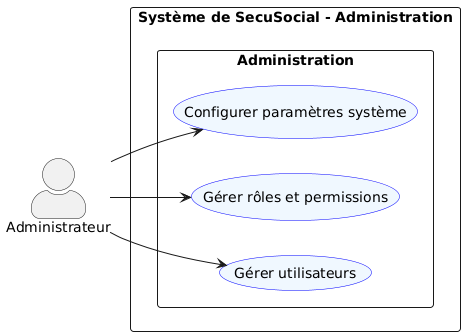
\includegraphics[width=0.5\textwidth]{AdminUC.png}
\caption{Diagramme de cas d'utilisation - Administrateur}
\end{figure}

\newpage

\noindent Le deuxième diagramme illustre les fonctionnalités accessibles aux contacts des entreprises clientes. Ils peuvent gérer les informations de \textbf{leur entreprise}, \textbf{leurs travailleurs} et \textbf{créer et suivre des demandes DIMONA}.

\vspace{0.5cm}
\begin{figure}[h]
\centering
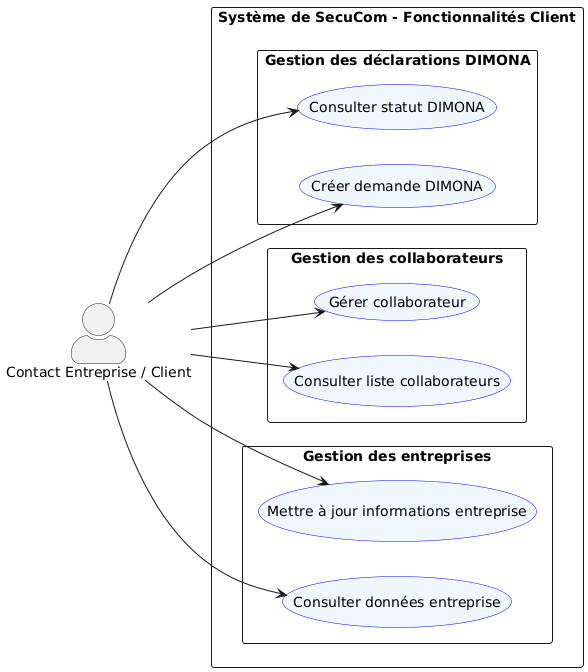
\includegraphics[width=0.5\textwidth]{ClientUC.png}
\caption{Diagramme de cas d'utilisation - Client}
\end{figure}

\noindent Le troisième diagramme présente les fonctionnalités accessibles aux employés du secrétariat social. Ils disposent d'un accès étendu pour \textbf{gérer les entreprises clientes}, \textbf{leurs travailleurs} et \textbf{traiter les demandes DIMONA ainsi que leurs statuts}. Le système intervient également pour certaines actions automatisées comme les notifications.

\vspace{0.5cm}
\begin{figure}[h]
\centering
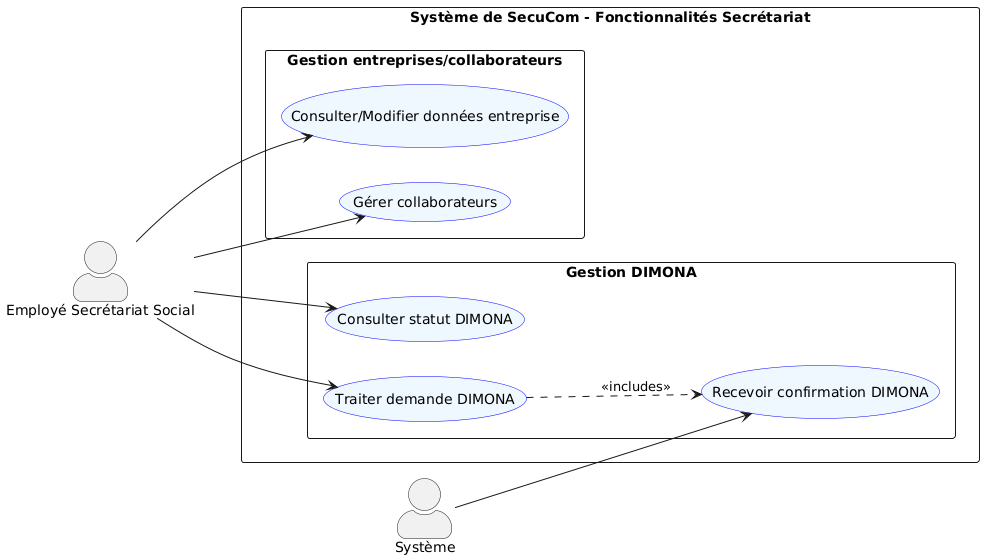
\includegraphics[width=0.5\textwidth]{SecretariatUC.png}
\caption{Diagramme de cas d'utilisation - Secrétariat Social}
\end{figure}

\section{Exigences et besoins techniques, de sécurité et de performance}

\subsection{Besoins techniques}

L'architecture technique de SecuCom doit répondre aux exigences spécifiques d'un secrétariat social tout en garantissant évolutivité, maintenabilité et robustesse. Les besoins techniques identifiés sont les suivants :

\vspace{0.5cm}
\textbf{Architecture globale} :
\begin{itemize}[leftmargin=*,label=\textcolor{darkgray}{$\bullet$},itemsep=0.3em]
  \item Architecture permettant une séparation claire entre l'interface utilisateur et la logique métier
  \item Communication efficace entre les différentes couches du système
  \item Flexibilité dans les options de déploiement selon les besoins
\end{itemize}


\vspace{0.5cm}
\textbf{Interface utilisateur} :
\begin{itemize}[leftmargin=*,label=\textcolor{darkgray}{$\bullet$},itemsep=0.3em]
  \item Interface intuitive et facile à prendre en main
  \item Adaptation à différentes tailles d'écran desktop (pas d'optimisation mobile requise)
  \item Gestion efficace des états et des données affichées
\end{itemize}


\vspace{0.5cm}
\textbf{Traitement des données} :
\begin{itemize}[leftmargin=*,label=\textcolor{darkgray}{$\bullet$},itemsep=0.3em]
  \item Système robuste de gestion de l'authentification et des autorisations
  \item Mécanismes efficaces pour l'accès et la persistance des données
  \item Solution adaptée pour le stockage sécurisé des données structurées
\end{itemize}


\vspace{0.5cm}
\textbf{Environnement de développement} :
\begin{itemize}[leftmargin=*,label=\textcolor{darkgray}{$\bullet$},itemsep=0.3em]
  \item Gestion de version pour le suivi des modifications
  \item Processus de build automatisé pour faciliter le développement
\end{itemize}

\subsection{Besoins de sécurité}

La sécurité est un aspect fondamental de SecuCom, étant donné la nature sensible des données traitées. Les exigences de sécurité suivantes ont été identifiées :


\vspace{0.5cm}
\textbf{Authentification et autorisation} :
\begin{itemize}[leftmargin=*,label=\textcolor{darkgray}{$\bullet$},itemsep=0.3em]
  \item Système d'authentification sécurisé avec gestion de jetons d'accès
  \item Gestion fine des rôles et permissions pour différents types d'utilisateurs
  \item Séparation stricte des espaces de données entre les différentes entreprises clientes
  \item Validation systématique des permissions à chaque requête
\end{itemize}


\newpage
\textbf{Protection des données} :
\begin{itemize}[leftmargin=*,label=\textcolor{darkgray}{$\bullet$},itemsep=0.3em]
  \item Transmission sécurisée des données via des protocoles chiffrés
  \item Gestion appropriée des exceptions pour éviter la fuite d'informations sensibles
  \item Conformité au RGPD (Règlement Général sur la Protection des Données)
\end{itemize}


\vspace{0.5cm}
\textbf{Sécurité applicative} :
\begin{itemize}[leftmargin=*,label=\textcolor{darkgray}{$\bullet$},itemsep=0.3em]
  \item Protection contre les attaques courantes (XSS, CSRF, injection SQL)
  \item Validation rigoureuse des entrées utilisateur
  \item Gestion sécurisée des mots de passe avec techniques de hachage appropriées
  \item Mécanisme de rafraîchissement des jetons d'authentification
\end{itemize}

\subsection{Besoins de performance}

Bien qu'aucune restriction spécifique n'ait été définie en termes de performance, SecuCom doit offrir une expérience utilisateur fluide et réactive pour garantir son adoption par les utilisateurs. Les exigences suivantes ont été établies :


\vspace{0.5cm}
\textbf{Temps de réponse} :
\begin{itemize}[leftmargin=*,label=\textcolor{darkgray}{$\bullet$},itemsep=0.3em]
  \item Chargement initial de l'application < 3 secondes
  \item Temps de réponse des requêtes < 1 seconde pour les opérations courantes
  \item Affichage des listes et tableaux optimisé
\end{itemize}


\vspace{0.5cm}
\textbf{Capacité et évolutivité} :
\begin{itemize}[leftmargin=*,label=\textcolor{darkgray}{$\bullet$},itemsep=0.3em]
  \item Capacité à gérer la croissance du nombre d'entreprises clientes et de collaborateurs
  \item Architecture permettant l'évolutivité en cas de besoin
\end{itemize}


\vspace{0.5cm}
\textbf{Optimisation} :
\begin{itemize}[leftmargin=*,label=\textcolor{darkgray}{$\bullet$},itemsep=0.3em]
  \item Requêtes optimisées pour les opérations courantes
\end{itemize}

\vspace{1cm}

\begin{tcolorbox}[
  title={\textbf{Cadre des exigences}},
  colback=blue!5!white,
  colframe=primarycolor,
  fonttitle=\bfseries,
  boxrule=0.5mm,
  arc=2mm,
  left=6mm,
  right=6mm,
  top=6mm,
  bottom=6mm
]
Ces exigences techniques, de sécurité et de performance constituent le cadre dans lequel SecuCom doit être développé, garantissant une solution robuste, sécurisée et performante qui répond aux besoins spécifiques de Sodabel et potentiellement d'autres secrétariats sociaux de taille similaire à l'avenir.
\end{tcolorbox}


% Analyse
\chapter{Analyse}

\noindent Cette section présente une analyse détaillée de l'architecture et du fonctionnement de \textbf{SecuCom}. À travers différents diagrammes UML, nous allons explorer la structure du système, ses composants, les relations entre les entités, ainsi que les flux d'interactions entre les différents acteurs et le système.

\section{Diagramme de composants}

\noindent Le diagramme de composants ci-dessous illustre l'architecture modulaire de \textbf{SecuCom}, mettant en évidence les principaux modules du système, leurs sous-composants et leurs interactions.

\begin{figure}[H]
\centering
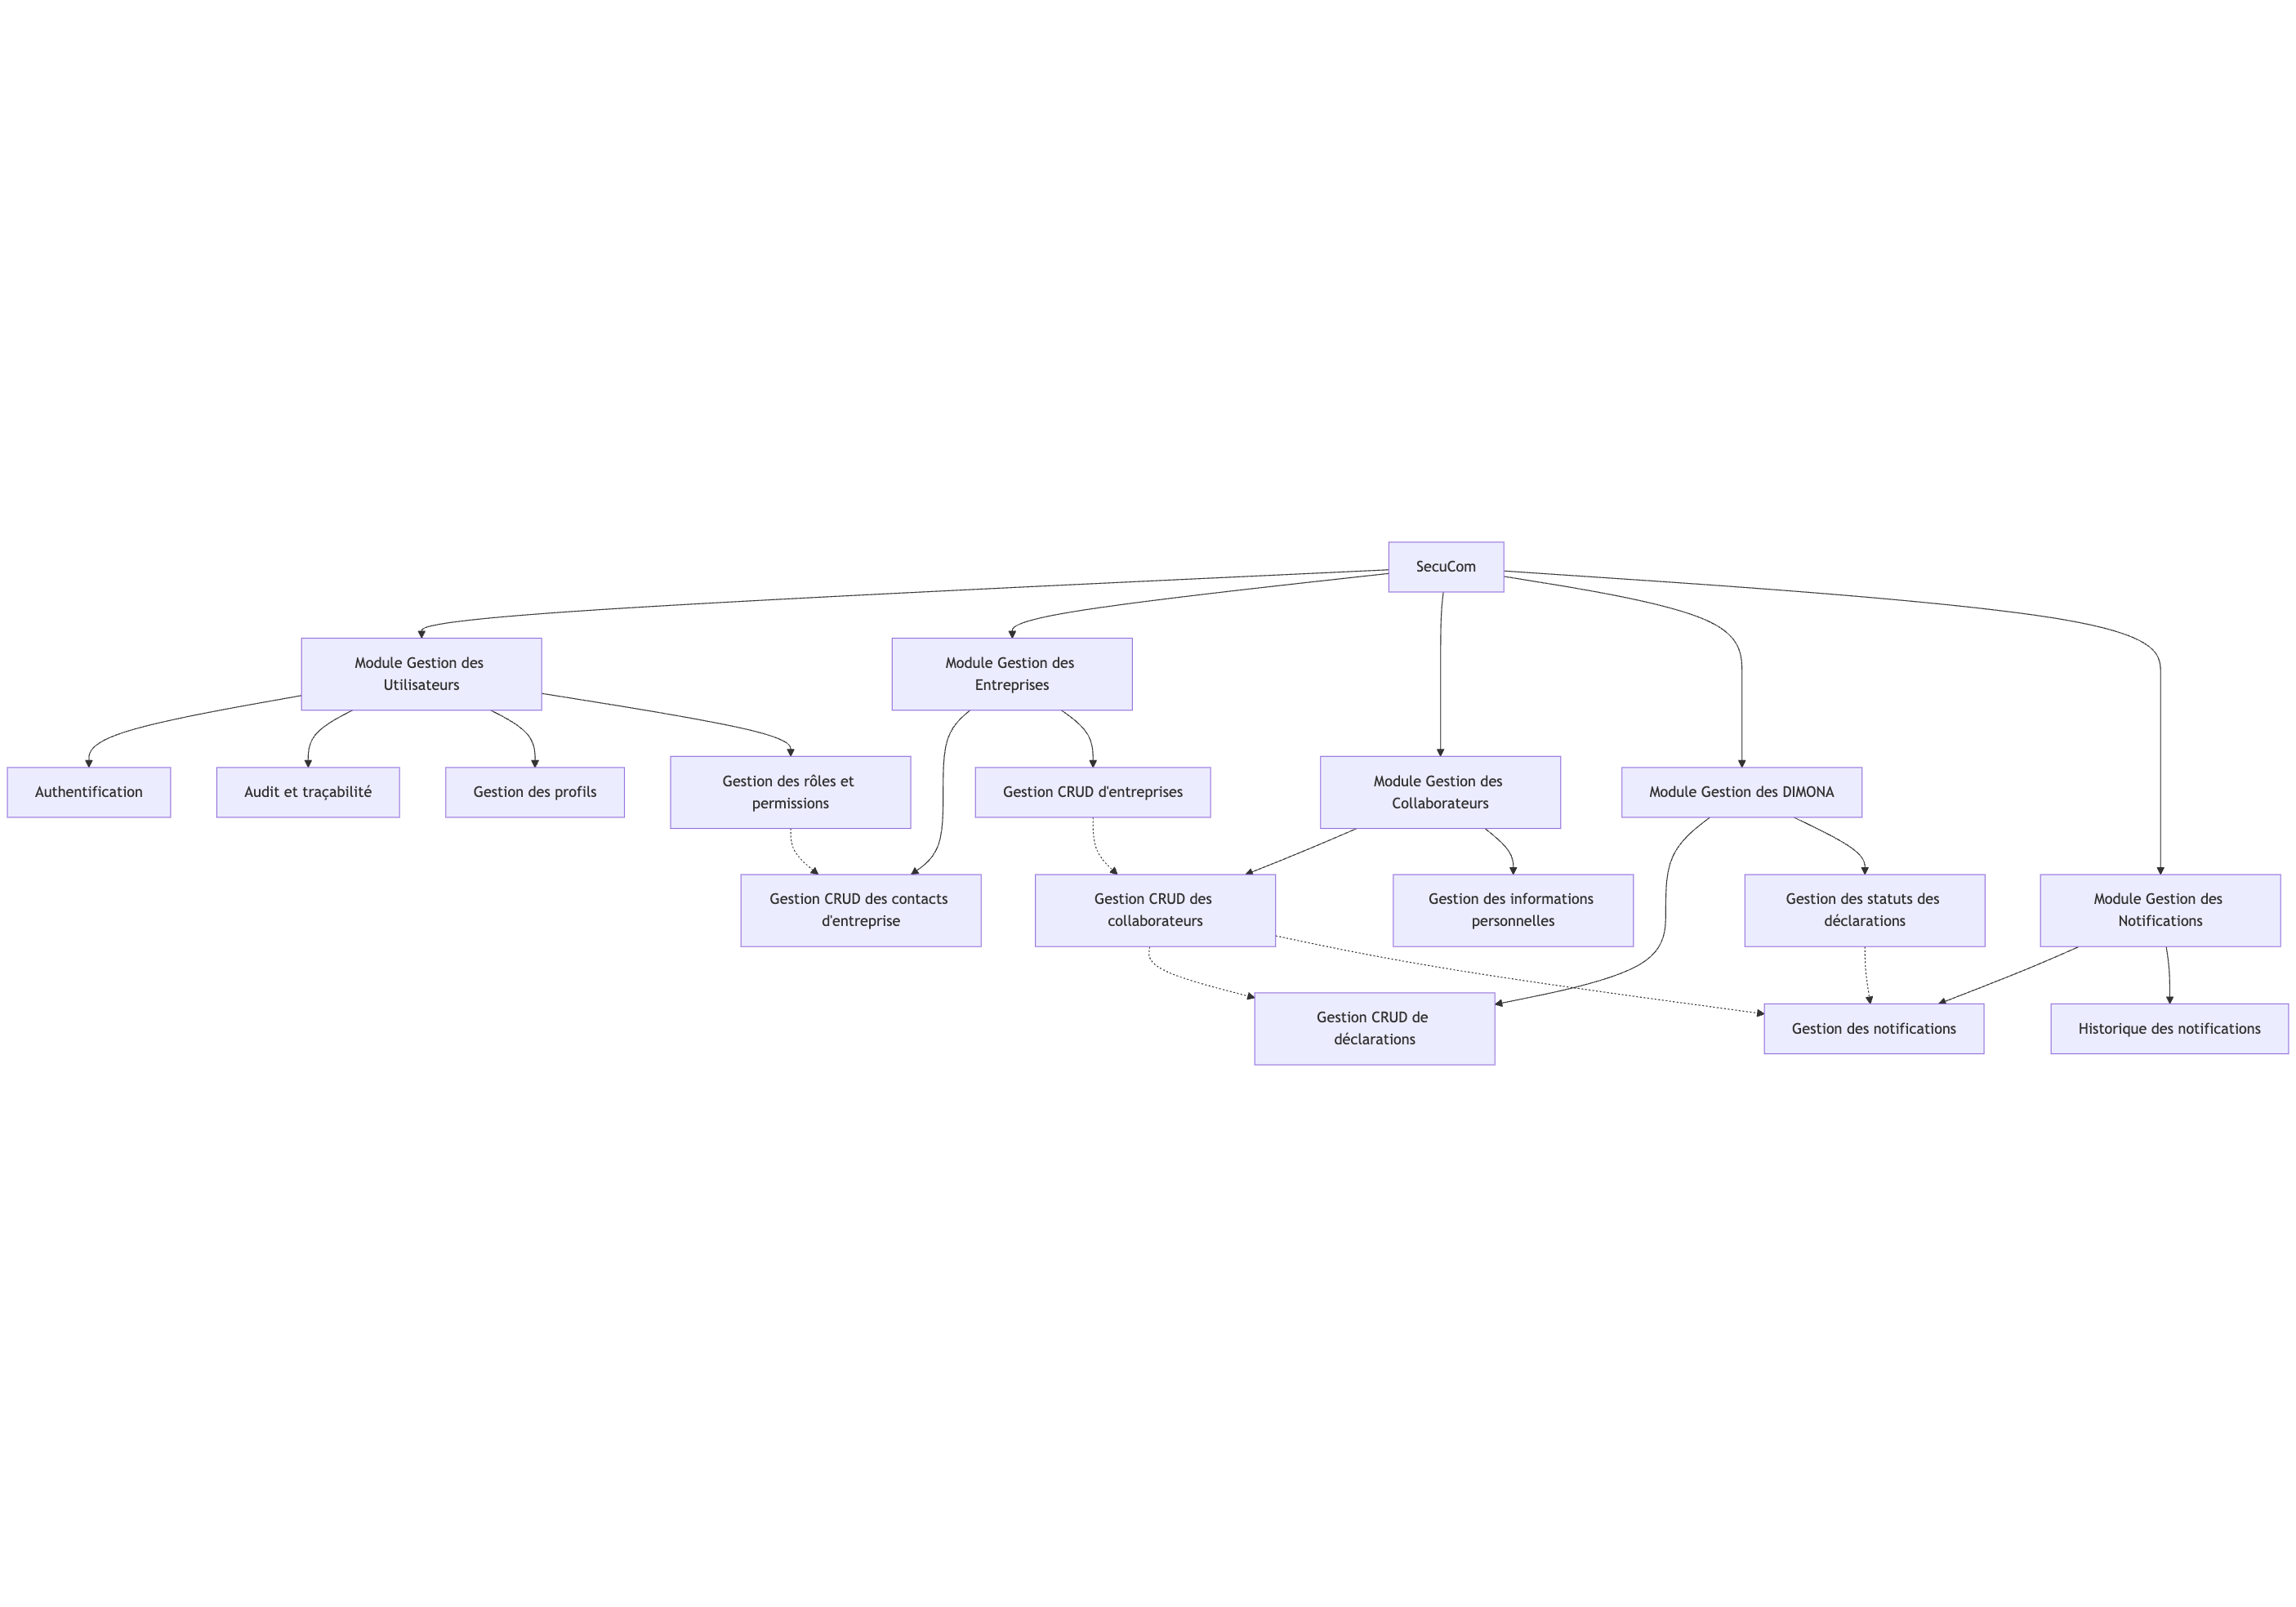
\includegraphics[width=0.9\textwidth]{ComposantsDiagram.png}
\caption{Diagramme de composants de SecuCom}
\end{figure}

\vspace{0.5cm}

\noindent Le système \textbf{SecuCom} est structuré autour de cinq modules principaux, chacun responsable d'un aspect spécifique de la plateforme :

\begin{itemize}[leftmargin=*,label=\textcolor{darkgray}{$\bullet$},itemsep=0.3em]
  \item \textbf{Module Gestion des Utilisateurs} : Comprend quatre sous-composants critiques :
    \begin{itemize}[leftmargin=*,label=\textcolor{darkgray}{$\bullet$},itemsep=0.3em]
      \item \textit{Authentification} : Gère la vérification des identités des utilisateurs.
      \item \textit{Audit et traçabilité} : Enregistre les actions des utilisateurs pour des fins de sécurité.
      \item \textit{Gestion des profils} : Permet la création, modification et suppression des profils utilisateurs.
      \item \textit{Gestion des rôles et permissions} : Définit et gère les droits d'accès aux différentes fonctionnalités.
    \end{itemize}
  
  \item \textbf{Module Gestion des Entreprises} : Comprend deux sous-composants essentiels :
    \begin{itemize}[leftmargin=*,label=\textcolor{darkgray}{$\bullet$},itemsep=0.3em]
      \item \textit{Gestion CRUD d'entreprises} : Gère le cycle de vie complet des entités entreprises (création, lecture, mise à jour, suppression).
      \item \textit{Gestion CRUD des contacts d'entreprise} : Administre les utilisateurs associés à chaque entreprise.
    \end{itemize}
  
  \item \textbf{Module Gestion des Collaborateurs} : Se compose de deux sous-composants :
    \begin{itemize}[leftmargin=*,label=\textcolor{darkgray}{$\bullet$},itemsep=0.3em]
      \item \textit{Gestion CRUD des collaborateurs} : Gère les travailleurs associés aux entreprises.
      \item \textit{Gestion des informations personnelles} : Administre les données personnelles des collaborateurs.
    \end{itemize}
  
  \item \textbf{Module Gestion des DIMONA} : Divisé en deux sous-composants :
    \begin{itemize}[leftmargin=*,label=\textcolor{darkgray}{$\bullet$},itemsep=0.3em]
      \item \textit{Gestion CRUD de déclarations} : Permet l'initiation, la consultation, la modification et la suppression des déclarations DIMONA.
      \item \textit{Gestion des statuts des déclarations} : Offre une visibilité sur l'état des déclarations en cours.
    \end{itemize}
    
  \item \textbf{Module Gestion des Notifications} : Comprend deux sous-composants :
    \begin{itemize}[leftmargin=*,label=\textcolor{darkgray}{$\bullet$},itemsep=0.3em]
      \item \textit{Gestion des notifications} : Gère l'envoi et le traitement des notifications.
      \item \textit{Historique des notifications} : Conserve un historique des notifications envoyées pour référence et suivi.
    \end{itemize}
\end{itemize}

\vspace{0.5cm}

\noindent Le diagramme met également en évidence des relations de dépendance importantes entre certains sous-composants :
\begin{itemize}[leftmargin=*,label=\textcolor{darkgray}{$\bullet$},itemsep=0.3em]
  \item La gestion d'entreprises (\textit{Gestion CRUD d'entreprises}) est liée à la gestion des collaborateurs (\textit{Gestion CRUD des collaborateurs}), illustrant le flux de travail où une entreprise doit exister avant de pouvoir y associer des collaborateurs.
  \item De même, la gestion des collaborateurs est liée à la gestion des déclarations DIMONA, reflétant la nécessité d'avoir un collaborateur enregistré avant de pouvoir effectuer une déclaration le concernant.
  \item La gestion des statuts des déclarations (\textit{Gestion des statuts des déclarations}) est liée à la gestion des notifications (\textit{Gestion des notifications}), permettant d'envoyer des notifications automatiques lorsqu'une déclaration DIMONA est créée ou change de statut.
  \item La gestion des collaborateurs (\textit{Gestion CRUD des collaborateurs}) est également liée à la gestion des notifications (\textit{Gestion des notifications}), permettant d'envoyer des notifications automatiques lorsqu'un nouveau collaborateur est créé.
\end{itemize}

\vspace{0.5cm}

\begin{tcolorbox}[
  title={\textbf{Architecture modulaire de SecuCom}},
  colback=blue!5!white,
  colframe=primarycolor,
  fonttitle=\bfseries,
  boxrule=0.5mm,
  arc=2mm,
  left=6mm,
  right=6mm,
  top=6mm,
  bottom=6mm
]
Cette architecture modulaire facilite la maintenance et l'évolution du système, chaque module pouvant être développé, testé et mis à jour de manière relativement indépendante, tout en préservant les interactions nécessaires entre les différentes fonctionnalités.
\end{tcolorbox}

\section{Diagramme de classes}

\noindent Le diagramme de classes ci-dessous représente les principales entités du système \textbf{SecuCom} et leurs relations. Il a été optimisé pour montrer clairement les classes actuellement utilisées dans l'implémentation et leurs relations.

\begin{figure}[H]
\centering
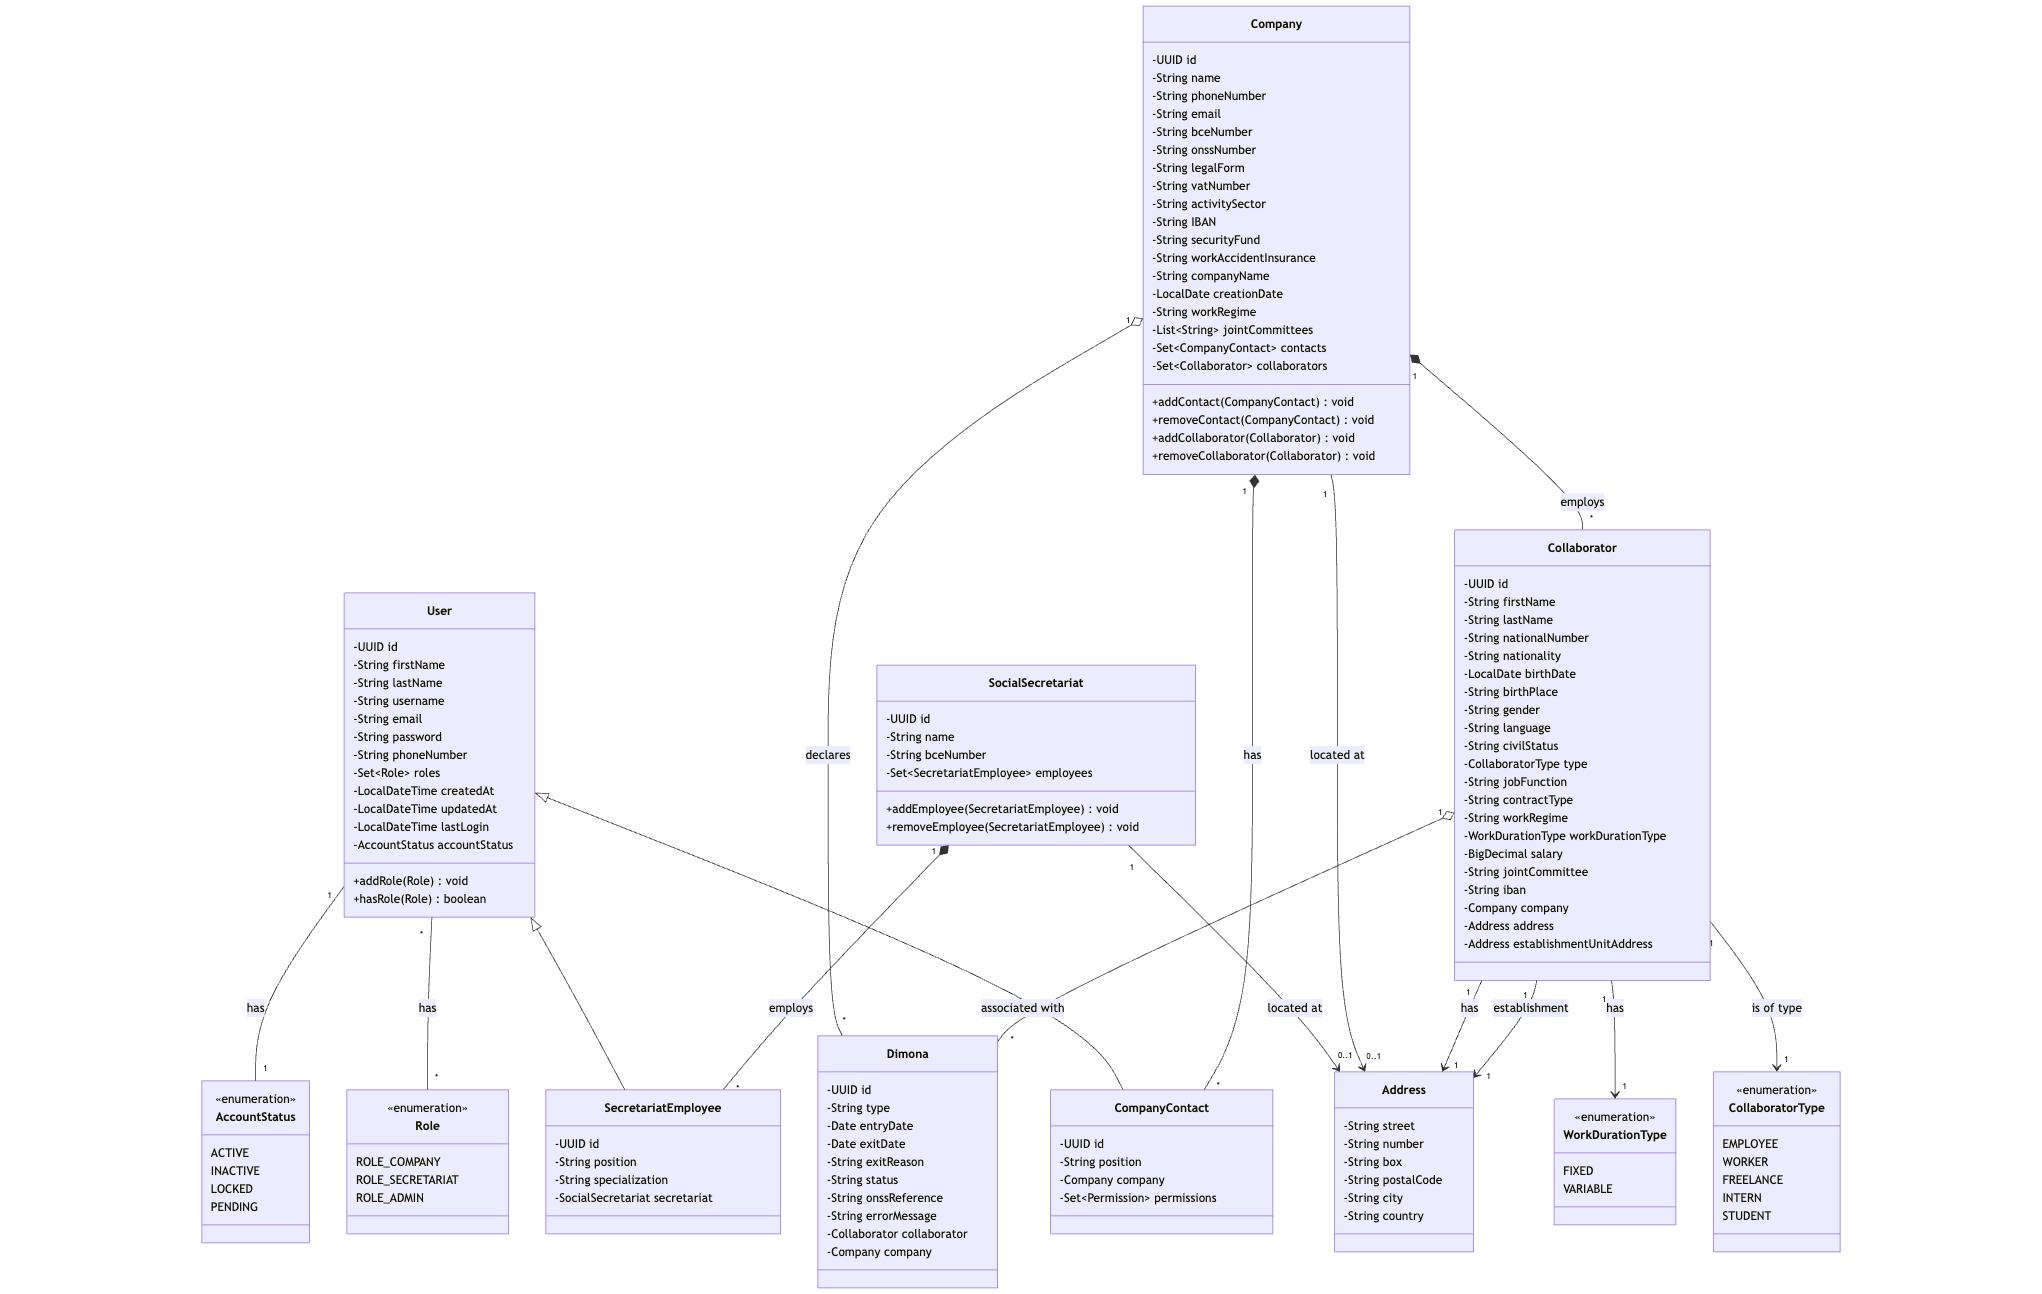
\includegraphics[width=0.9\textwidth]{ClassDiagram.png}
\caption{Diagramme de classes de SecuCom}
\end{figure}

\vspace{0.5cm}

\noindent Les principales classes du système sont :

\begin{itemize}[leftmargin=*,label=\textcolor{darkgray}{$\bullet$},itemsep=0.3em]
  \item \textbf{User} : Classe de base pour tous les utilisateurs du système, avec des attributs comme id, email, password, firstName, lastName, etc. Elle est associée à des rôles (Role) et à un statut de compte (AccountStatus).

  \item \textbf{Role} : Énumération définissant les différents rôles disponibles dans le système (ROLE\_COMPANY, ROLE\_SECRETARIAT, ROLE\_ADMIN).

  \item \textbf{AccountStatus} : Énumération définissant les différents états possibles d'un compte utilisateur (ACTIVE, INACTIVE, LOCKED, PENDING).

  \item \textbf{SocialSecretariat} : Représente le secrétariat social avec ses informations et ses employés. Il peut avoir plusieurs employés (SecretariatEmployee) et est associé à une adresse (Address).

  \item \textbf{SecretariatEmployee} : Employé du secrétariat social, hérite de User et est associé à un secrétariat social (SocialSecretariat).

  \item \textbf{Company} : Entreprise cliente avec ses informations d'identification et ses contacts. Elle peut avoir plusieurs contacts (CompanyContact), plusieurs collaborateurs (Collaborator) et plusieurs déclarations DIMONA (Dimona). Elle est également associée à une adresse (Address).

  \item \textbf{CompanyContact} : Contact au sein d'une entreprise cliente, hérite de User et est associé à une entreprise (Company).

  \item \textbf{Collaborator} : Travailleur d'une entreprise cliente avec ses informations personnelles et professionnelles. Il est associé à une entreprise (Company), à une adresse personnelle (Address), à une adresse d'établissement (Address), à un type de collaborateur (CollaboratorType) et à un type de durée de travail (WorkDurationType). Il peut avoir plusieurs déclarations DIMONA (Dimona).

  \item \textbf{CollaboratorType} : Énumération définissant les différents types de collaborateurs (EMPLOYEE, WORKER, FREELANCE, INTERN, STUDENT).

  \item \textbf{WorkDurationType} : Énumération définissant les différents types de durée de travail (FIXED, VARIABLE).

  \item \textbf{Dimona} : Déclaration DIMONA associée à un collaborateur (Collaborator) et à une entreprise (Company).

  \item \textbf{Address} : Adresse physique utilisée par plusieurs entités (Collaborator, Company, SocialSecretariat).
  
  \item \textbf{Notification} : Représente une notification envoyée à un utilisateur, avec des attributs comme id, message, type, read (lu/non lu), createdAt, recipient (destinataire) et entityId (référence à l'entité concernée).
  
  \item \textbf{NotificationType} : Énumération définissant les différents types de notifications (DIMONA\_CREATED, DIMONA\_STATUS\_CHANGED, COLLABORATOR\_CREATED).
\end{itemize}

Les relations entre ces classes sont clairement définies avec des multiplicités appropriées (one-to-many, many-to-many, etc.) et des noms de relations explicites pour faciliter la compréhension du modèle.

\newpage

\section{Diagramme d'entités relationnelles}

\noindent Le diagramme d'entités relationnelles (ERD) ci-dessous représente la structure de la base de données de \textbf{SecuCom}. Il montre les tables, leurs attributs et les relations entre elles.

\begin{figure}[H]
\centering
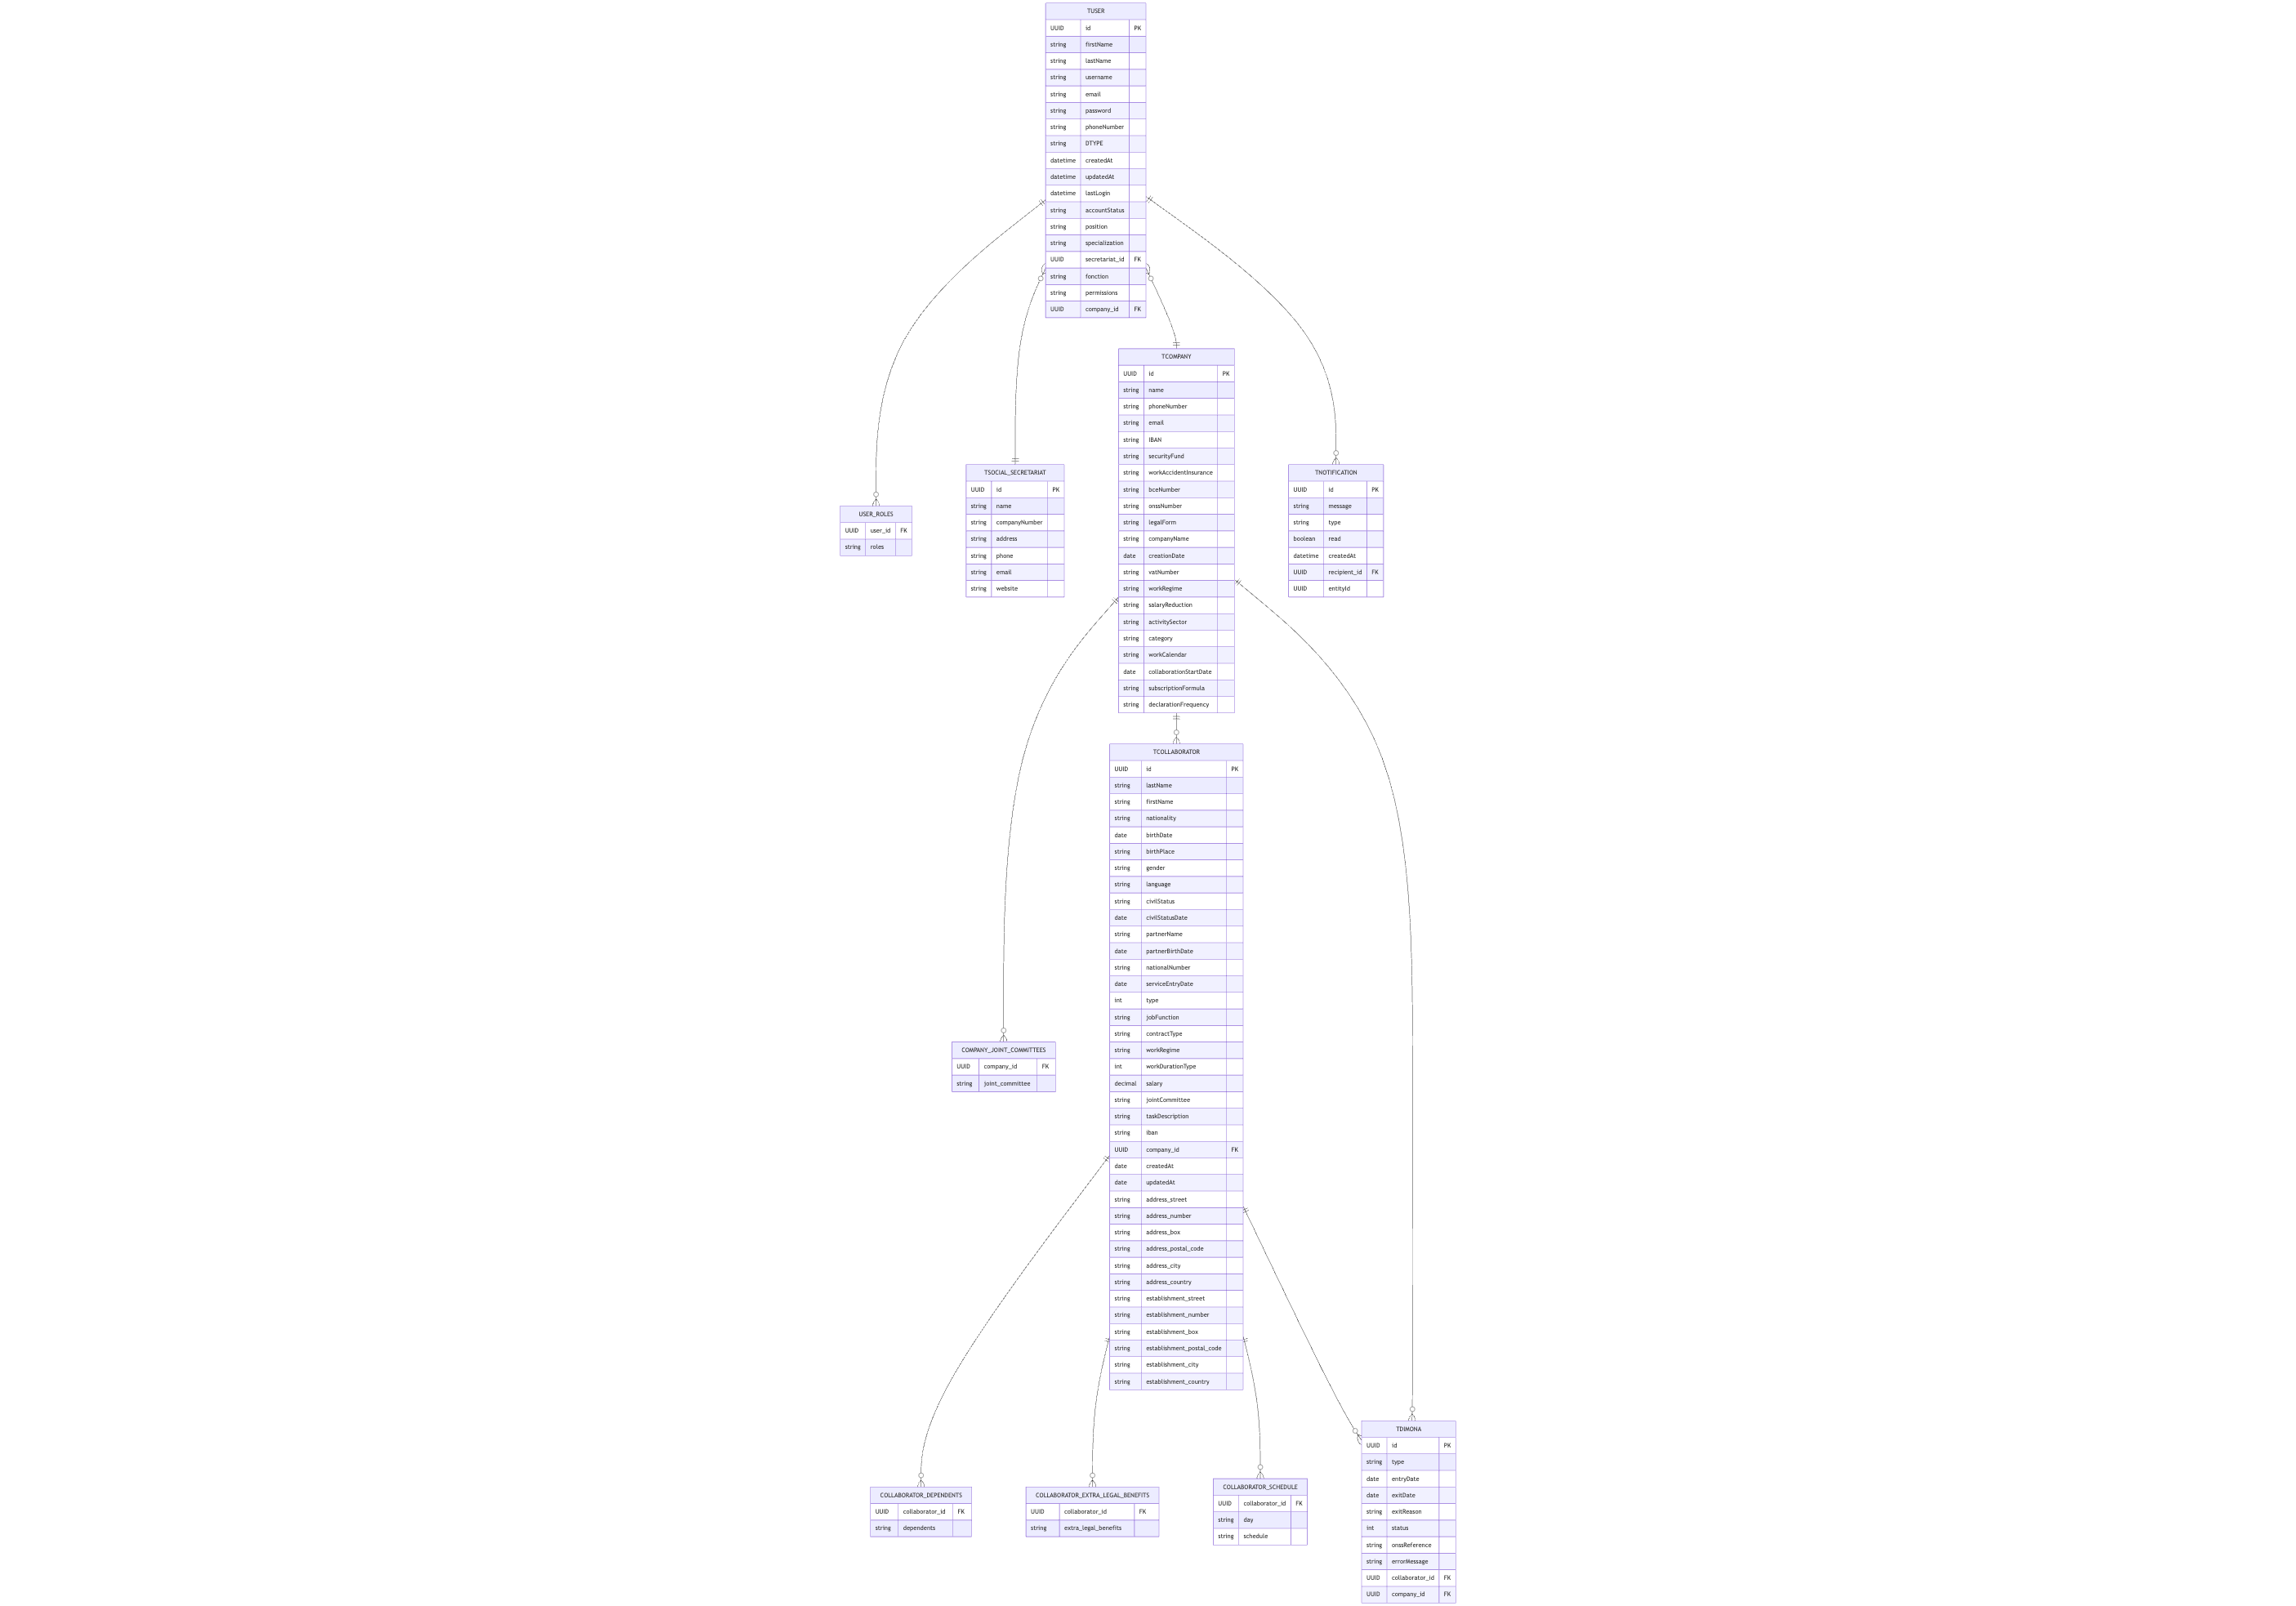
\includegraphics[width=0.9\textwidth]{ERD.png}
\caption{Diagramme d'entités relationnelles de SecuCom}
\end{figure}

\vspace{0.5cm}

\noindent Les principales entités de la base de données sont :

\begin{itemize}[leftmargin=*,label=\textcolor{darkgray}{$\bullet$},itemsep=0.3em]
  \item \textbf{TUSER} : Stocke les informations de base des utilisateurs (identifiant, email, mot de passe, nom, prénom, etc.). Cette table utilise l'héritage par une colonne discriminante (DTYPE) pour distinguer les différents types d'utilisateurs.

  \item \textbf{USER\_ROLES} : Table de jointure qui associe les utilisateurs à leurs rôles.

  \item \textbf{TSOCIAL\_SECRETARIAT} : Stocke les informations des secrétariats sociaux (nom, numéro d'entreprise, adresse, téléphone, email, site web).

  \item \textbf{TCOMPANY} : Stocke les informations des entreprises clientes (nom, téléphone, email, IBAN, numéro BCE, numéro ONSS, forme juridique, etc.).

  \item \textbf{COMPANY\_JOINT\_COMMITTEES} : Stocke les commissions paritaires associées aux entreprises.

  \item \textbf{TCOLLABORATOR} : Stocke les informations des travailleurs des entreprises clientes (nom, prénom, nationalité, date de naissance, lieu de naissance, genre, langue, état civil, numéro national, fonction, type de contrat, régime de travail, salaire, etc.).

  \item \textbf{COLLABORATOR\_DEPENDENTS} : Stocke les personnes à charge des collaborateurs.

  \item \textbf{COLLABORATOR\_EXTRA\_LEGAL\_BENEFITS} : Stocke les avantages extra-légaux des collaborateurs.

  \item \textbf{COLLABORATOR\_SCHEDULE} : Stocke les horaires de travail des collaborateurs.

  \item \textbf{TDIMONA} : Stocke les informations des déclarations DIMONA (type, date d'entrée, date de sortie, raison de sortie, statut, référence ONSS, message d'erreur, etc.).
  
  \item \textbf{TNOTIFICATION} : Stocke les notifications envoyées aux utilisateurs (message, type, statut de lecture, date de création, destinataire, référence à l'entité concernée).
\end{itemize}

\vspace{0.5cm}

\noindent Les relations entre ces entités sont les suivantes :

\begin{itemize}[leftmargin=*,label=\textcolor{darkgray}{$\bullet$},itemsep=0.3em]
  \item Un utilisateur peut avoir plusieurs rôles (relation one-to-many entre TUSER et USER\_ROLES).
  \item Un utilisateur peut être associé à un secrétariat social (relation many-to-one entre TUSER et TSOCIAL\_SECRETARIAT).
  \item Un utilisateur peut être associé à une entreprise (relation many-to-one entre TUSER et TCOMPANY).
  \item Une entreprise peut avoir plusieurs commissions paritaires (relation one-to-many entre TCOMPANY et COMPANY\_JOINT\_COMMITTEES).
  \item Une entreprise peut avoir plusieurs collaborateurs (relation one-to-many entre TCOMPANY et TCOLLABORATOR).
  \item Une entreprise peut avoir plusieurs déclarations DIMONA (relation one-to-many entre TCOMPANY et TDIMONA).
  \item Un collaborateur peut avoir plusieurs personnes à charge (relation one-to-many entre TCOLLABORATOR et COLLABORATOR\_DEPENDENTS).
  \item Un collaborateur peut avoir plusieurs avantages extra-légaux (relation one-to-many entre TCOLLABORATOR et COLLABORATOR\_EXTRA\_LEGAL\_BENEFITS).
  \item Un collaborateur peut avoir plusieurs horaires de travail (relation one-to-many entre TCOLLABORATOR et COLLABORATOR\_SCHEDULE).
  \item Un collaborateur peut avoir plusieurs déclarations DIMONA (relation one-to-many entre TCOLLABORATOR et TDIMONA).
  \item Un utilisateur peut recevoir plusieurs notifications (relation one-to-many entre TUSER et TNOTIFICATION).
\end{itemize}

\vspace{0.5cm}

\textbf{Champs obligatoires (NOT NULL):}
\begin{itemize}[leftmargin=*,label=\textcolor{darkgray}{$\bullet$},itemsep=0.3em]
  \item USER: firstName, lastName, username, email, password, roles, createdAt, accountStatus
  \item SOCIAL\_SECRETARIAT: name, companyNumber
  \item COMPANY: name
  \item COLLABORATOR: lastName, firstName, serviceEntryDate, company\_id, createdAt
  \item DIMONA: collaborator\_id, company\_id
\end{itemize}

\vspace{0.5cm}

\textbf{Contraintes d'unicité (UNIQUE):}
\begin{itemize}[leftmargin=*,label=\textcolor{darkgray}{$\bullet$},itemsep=0.3em]
  \item USER: username, email
  \item COMPANY: bceNumber, onssNumber, vatNumber
  \item COLLABORATOR: nationalNumber
\end{itemize}

\vspace{0.5cm}

\textbf{Types énumérés:}
\begin{itemize}[leftmargin=*,label=\textcolor{darkgray}{$\bullet$},itemsep=0.3em]
  \item USER.accountStatus: ACTIVE (défaut), INACTIVE, LOCKED, PENDING
  \item COLLABORATOR.type: EMPLOYEE, WORKER, FREELANCE, INTERN, STUDENT
  \item COLLABORATOR.workDurationType: FIXED, VARIABLE
  \item NOTIFICATION.type: DIMONA\_CREATED, DIMONA\_STATUS\_CHANGED, COLLABORATOR\_CREATED
\end{itemize}

\vspace{0.5cm}

\begin{tcolorbox}[
  title={\textbf{Modèle de données robuste}},
  colback=blue!5!white,
  colframe=primarycolor,
  fonttitle=\bfseries,
  boxrule=0.5mm,
  arc=2mm,
  left=6mm,
  right=6mm,
  top=6mm,
  bottom=6mm
]
Ce modèle de données permet de représenter efficacement les relations complexes entre les différentes entités du système, tout en assurant l'intégrité des données et la performance des requêtes. La structure relationnelle facilite la gestion des associations entre entreprises, collaborateurs et déclarations DIMONA, tout en maintenant une séparation claire des responsabilités. Les mécanismes de suppression en cascade garantissent la cohérence des données en évitant les références orphelines.
\end{tcolorbox}

\newpage

\section{Diagrammes de séquences}

\noindent Les diagrammes de séquence ci-dessous illustrent les interactions entre les différents composants du système \textbf{SecuCom} pour les cas d'utilisation clés. Ces diagrammes permettent de visualiser clairement les flux de communication entre les acteurs et le système.

\begin{note}
Les diagrammes de séquence sont particulièrement utiles pour comprendre la dynamique temporelle des interactions et identifier les points de communication critiques entre les différentes parties du système.
\end{note}

\subsection{Cas d'utilisation : Création d'une entreprise}

\noindent Le diagramme de séquence ci-dessous illustre le processus de création d'une entreprise dans le système \textbf{SecuCom}. Ce processus implique trois acteurs principaux : l'Administrateur, le Contact Entreprise et l'Employé du Secrétariat Social.

\begin{figure}[H]
\centering
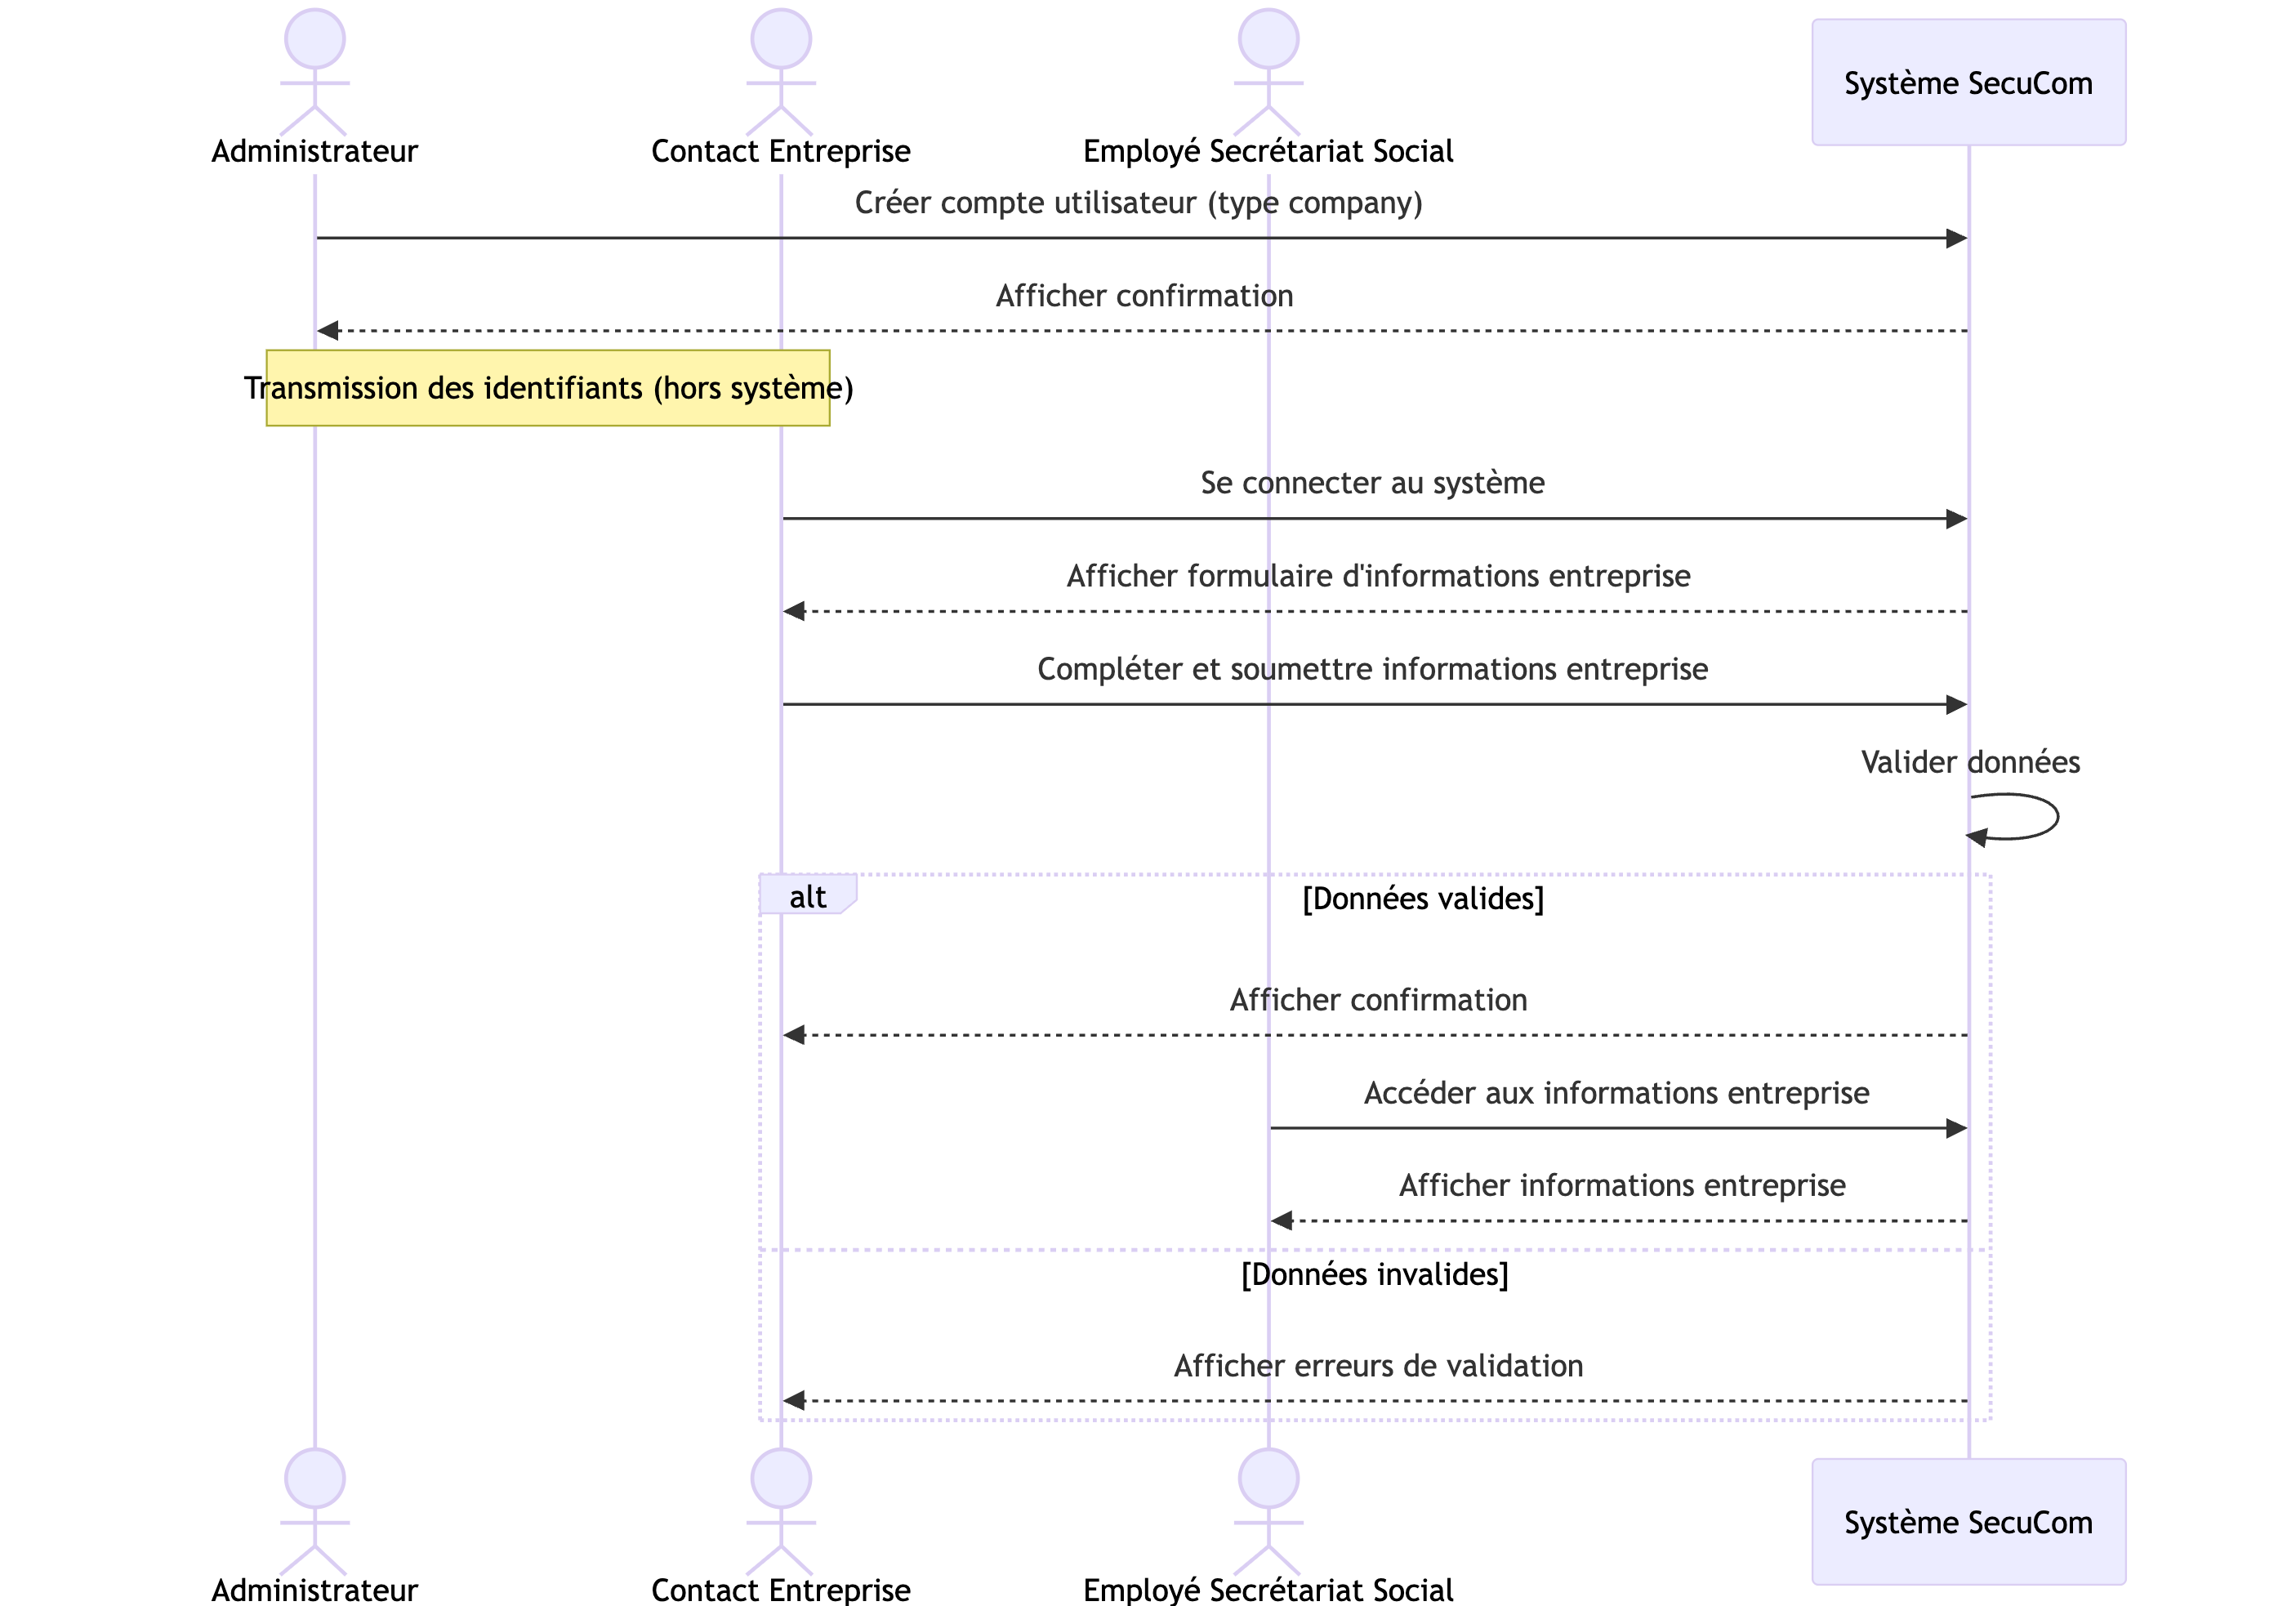
\includegraphics[width=0.9\textwidth]{SD_creation_entreprise.png}
\caption{Diagramme de séquence - Création d'une entreprise}
\end{figure}

\vspace{0.5cm}

\subsubsection{Description du processus}

\begin{enumerate}
  \item \textbf{Initialisation par l'Administrateur} :
    \begin{itemize}
      \item L'Administrateur crée un compte utilisateur de type "company" avec les données minimales obligatoires.
      \item Le système enregistre ces informations dans la base de données et confirme la création du compte.
    \end{itemize}

  \item \textbf{Transmission des identifiants} :
    \begin{itemize}
      \item L'Administrateur transmet les identifiants de connexion au Contact Entreprise (cette étape se déroule en dehors du système, par exemple par email ou téléphone).
    \end{itemize}

  \item \textbf{Complétion des informations par le Contact Entreprise} :
    \begin{itemize}
      \item Le Contact Entreprise se connecte au système avec les identifiants fournis.
      \item Le système affiche un formulaire permettant de compléter les informations de l'entreprise.
      \item Le Contact Entreprise saisit et soumet les informations complètes de son entreprise (nom, numéro BCE, numéro ONSS, numéro TVA, etc.).
      \item Le système valide les données soumises.
    \end{itemize}

  \item \textbf{Traitement des données} :
    \begin{itemize}
      \item Si les données sont valides, le système les enregistre dans la base de données et confirme l'enregistrement au Contact Entreprise.
      \item Si les données sont invalides, le système affiche les erreurs de validation au Contact Entreprise, qui doit les corriger et soumettre à nouveau.
    \end{itemize}

  \item \textbf{Accès par le Secrétariat Social} :
    \begin{itemize}
      \item L'Employé du Secrétariat Social peut accéder aux informations de l'entreprise.
      \item Le système récupère ces informations depuis la base de données et les affiche à l'Employé du Secrétariat Social.
    \end{itemize}
\end{enumerate}

\subsubsection{Avantages de cette approche}

Cette approche de création d'entreprise présente plusieurs avantages :
\begin{itemize}
  \item Elle responsabilise le Contact Entreprise pour la fourniture et la maintenance de ses propres informations.
  \item Elle réduit la charge administrative pour l'Administrateur et le Secrétariat Social.
  \item Elle améliore la précision des données puisqu'elles sont fournies directement par la source.
  \item Elle s'inscrit dans un modèle de self-service plus moderne et efficace.
  \item Elle facilite la scalabilité du système en permettant de gérer un plus grand nombre d'entreprises.
\end{itemize}

Ce processus constitue la première étape dans le cycle de vie d'une entreprise au sein du système SecuCom, et sert de fondation pour les autres cas d'utilisation comme l'ajout de collaborateurs et la création de déclarations DIMONA.

\subsection{Cas d'utilisation : Ajout d'un collaborateur}

\noindent Le diagramme de séquence ci-dessous illustre le processus d'ajout d'un collaborateur (employé) dans le système \textbf{SecuCom}. Ce processus implique plusieurs composants du système et inclut des validations importantes pour garantir l'intégrité des données.

\begin{figure}[H]
\centering
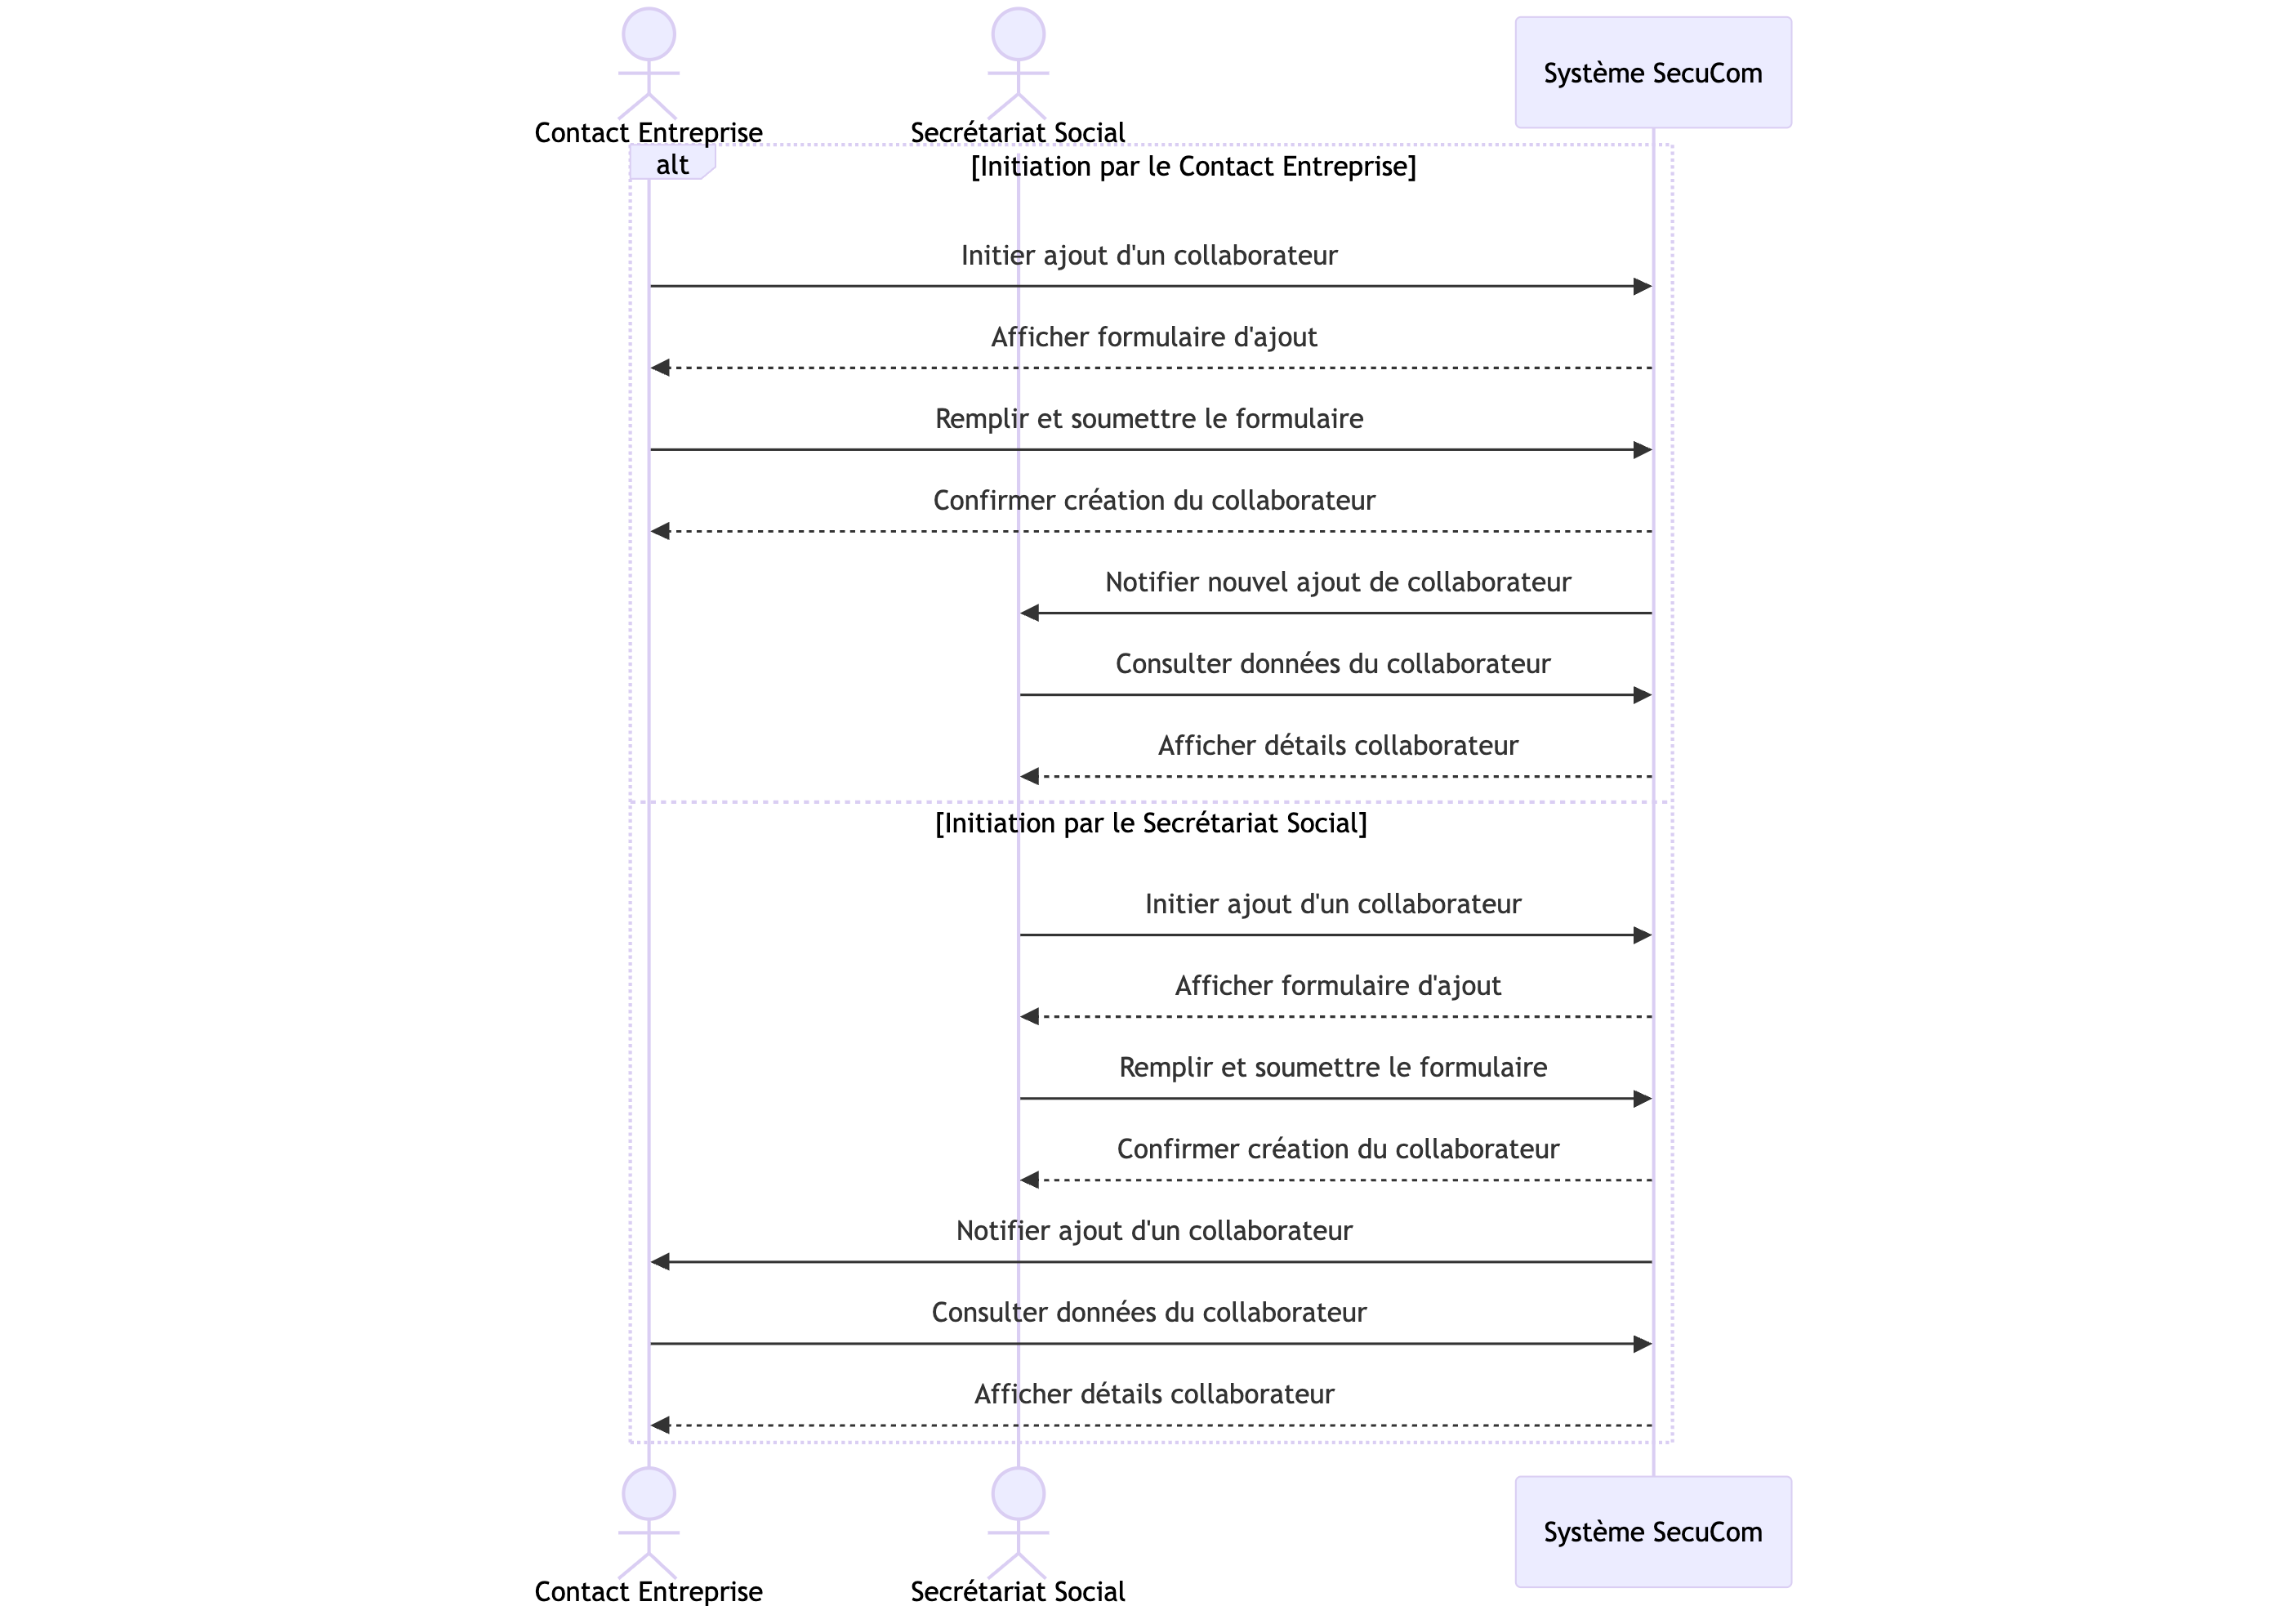
\includegraphics[width=0.9\textwidth]{SD_creation_collaborateur.png}
\caption{Diagramme de séquence - Ajout d'un collaborateur}
\end{figure}

\vspace{0.5cm}

\subsubsection{Description du processus}

\begin{enumerate}
  \item \textbf{Initiation de l'ajout} :
    \begin{itemize}
      \item \textbf{Scénario 1} : Le Contact Entreprise initie l'ajout d'un collaborateur, remplit le formulaire et soumet les données au système.
      \item \textbf{Scénario 2} : Le Secrétariat Social initie l'ajout d'un collaborateur, remplit le formulaire et soumet les données au système.
    \end{itemize}

  \item \textbf{Enregistrement des données} :
    \begin{itemize}
      \item Le système enregistre directement les informations du collaborateur dans la base de données.
      \item Une confirmation est envoyée à l'initiateur de la demande.
    \end{itemize}

  \item \textbf{Notification} :
    \begin{itemize}
      \item L'autre partie (celle qui n'a pas initié l'ajout) est notifiée de l'ajout du collaborateur.
      \item Elle peut consulter les détails du collaborateur ajouté.
    \end{itemize}
\end{enumerate}

\subsubsection{Aspects importants du processus}

Ce processus met en évidence plusieurs aspects importants du système SecuCom :

\begin{itemize}
  \item \textbf{Double flux d'initiation} : La flexibilité du système permet à deux types d'acteurs différents d'initier le processus selon les besoins et les préférences.
  \item \textbf{Simplicité du processus} : Le processus est simplifié pour permettre un ajout rapide et efficace des collaborateurs.
  \item \textbf{Communication bidirectionnelle} : Le système sert d'intermédiaire pour la communication entre le Contact Entreprise et le Secrétariat Social, facilitant le partage d'informations.
  \item \textbf{Traçabilité} : Toutes les étapes du processus sont enregistrées dans la base de données, permettant un suivi de l'historique des ajouts de collaborateurs.
\end{itemize}

L'ajout d'un collaborateur est une étape cruciale qui permet ensuite de procéder à d'autres opérations comme la création de déclarations DIMONA pour ce collaborateur.

\subsection{Cas d'utilisation : Création d'une déclaration DIMONA}

\noindent Le diagramme de séquence ci-dessous illustre le processus de création d'une déclaration DIMONA dans le système \textbf{SecuCom}. Ce processus peut être initié soit par le Contact Entreprise, soit par le Secrétariat Social, et implique une validation manuelle des données avant la soumission à l'ONSS.

\begin{figure}[H]
\centering
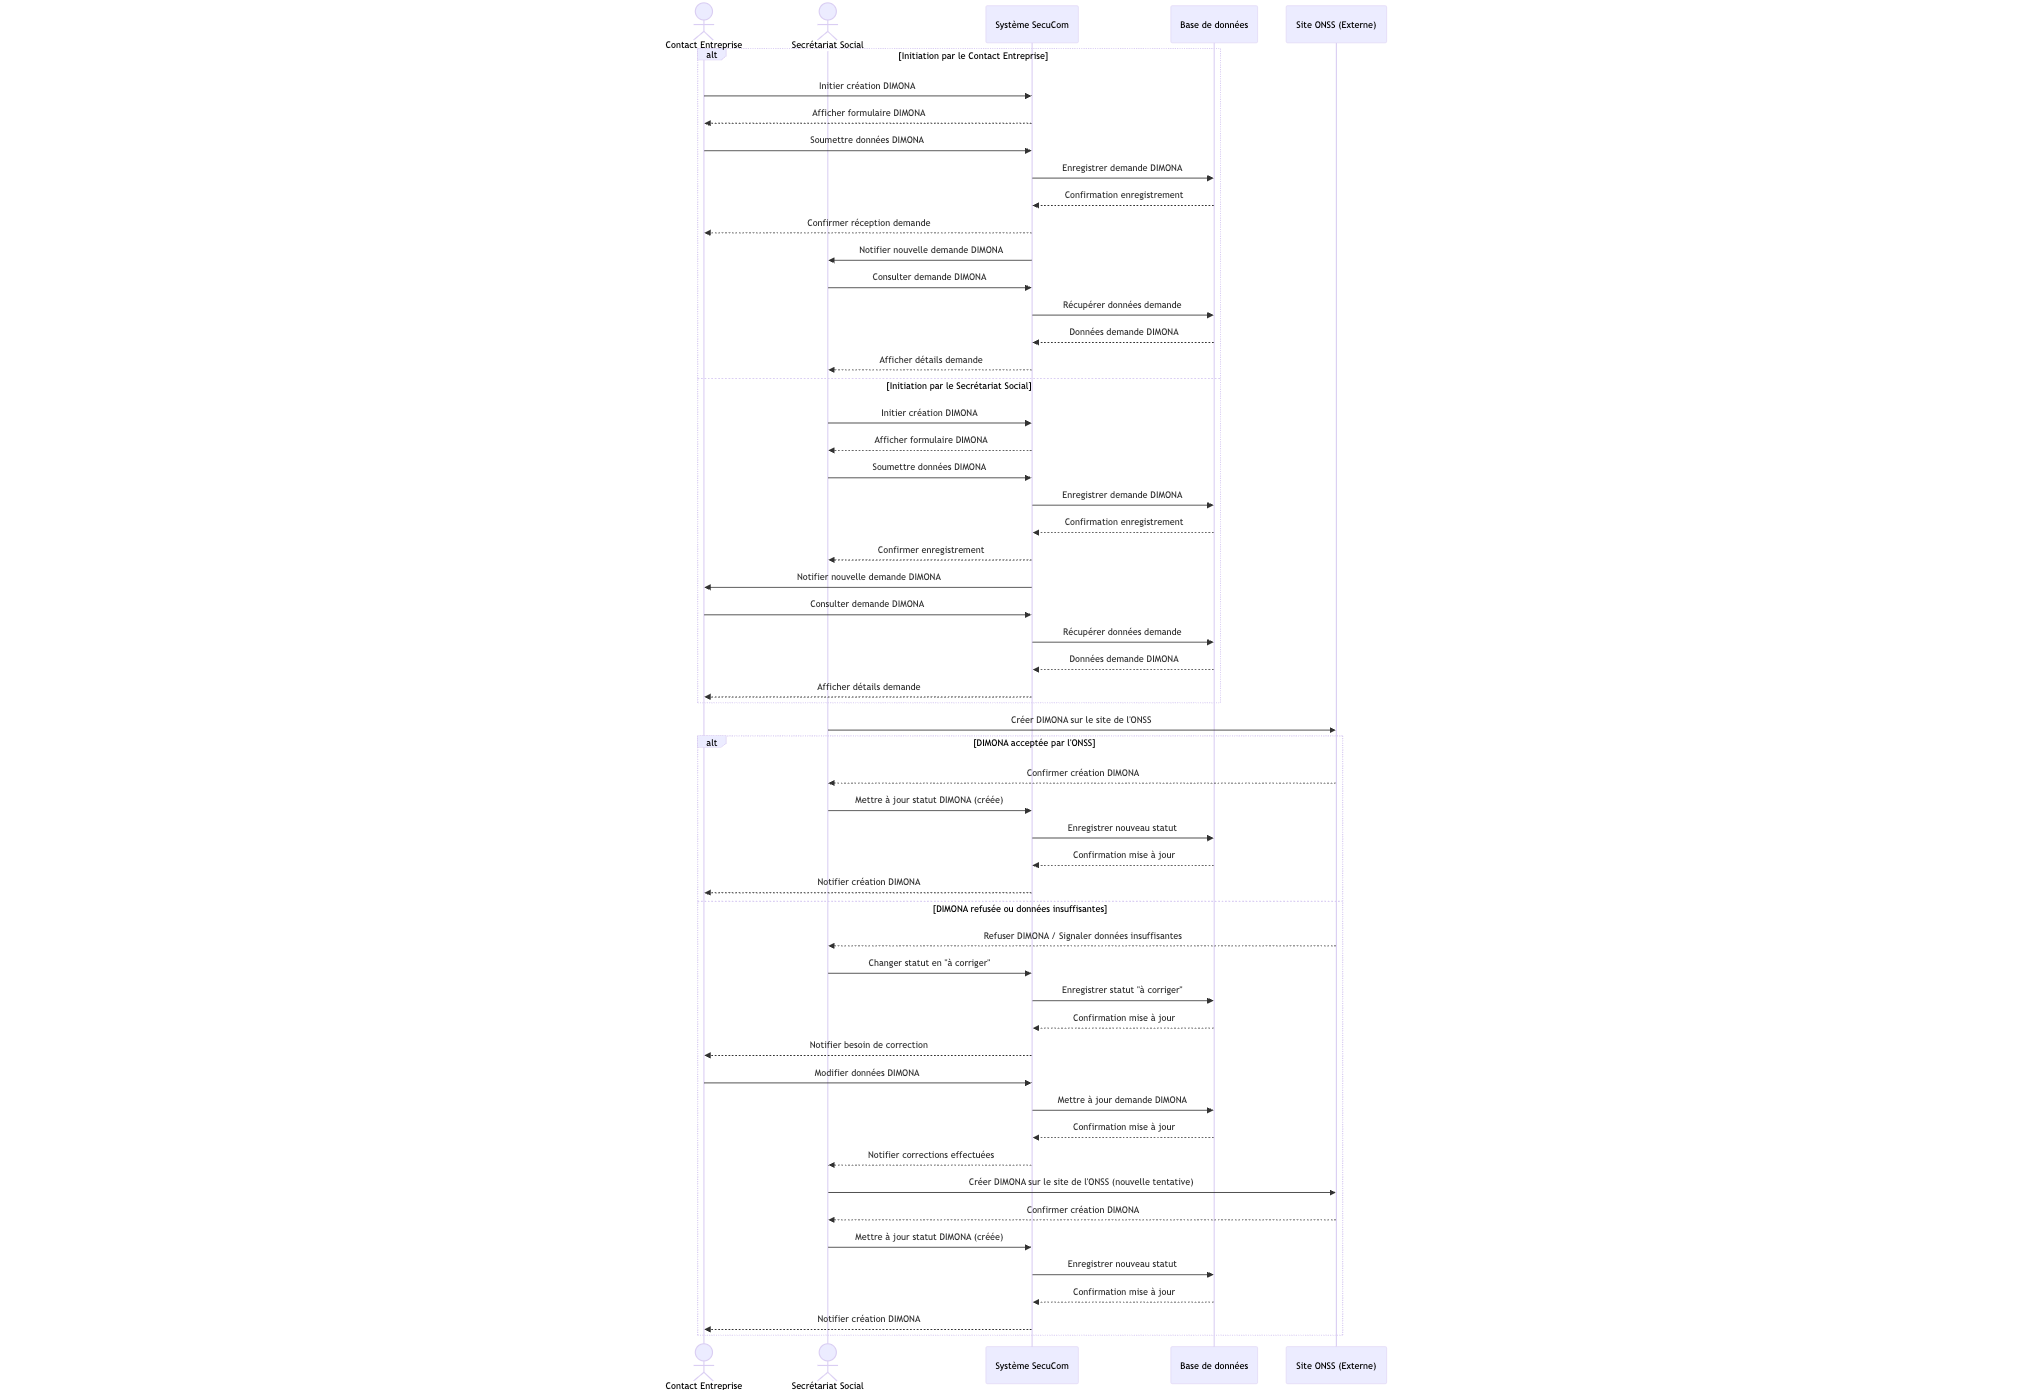
\includegraphics[width=0.9\textwidth]{SD_creation_dimona.png}
\caption{Diagramme de séquence - Création d'une déclaration DIMONA}
\end{figure}

\vspace{0.5cm}

\subsubsection{Description du processus}

\begin{enumerate}
  \item \textbf{Initiation de la demande} :
    \begin{itemize}
      \item \textbf{Scénario 1} : Le Contact Entreprise initie la création d'une déclaration DIMONA, remplit le formulaire et soumet les données au système.
      \item \textbf{Scénario 2} : Le Secrétariat Social initie la création d'une déclaration DIMONA, remplit le formulaire et soumet les données au système.
    \end{itemize}

  \item \textbf{Notification} :
    \begin{itemize}
      \item L'autre partie (celle qui n'a pas initié la demande) est notifiée de la nouvelle demande DIMONA.
      \item Elle peut consulter les détails de la demande.
    \end{itemize}

  \item \textbf{Création sur le site de l'ONSS} :
    \begin{itemize}
      \item Le Secrétariat Social crée la déclaration DIMONA sur le site officiel de l'ONSS.
    \end{itemize}

  \item \textbf{Traitement du résultat} :
    \begin{itemize}
      \item \textbf{Si la DIMONA est acceptée par l'ONSS} :
        \begin{itemize}
          \item L'ONSS confirme la création de la DIMONA.
          \item Le Secrétariat Social met à jour le statut dans le système.
          \item Le Contact Entreprise est notifié de la création effective de la DIMONA.
        \end{itemize}
      \item \textbf{Si la DIMONA est refusée ou les données sont insuffisantes} :
        \begin{itemize}
          \item L'ONSS refuse la DIMONA ou signale que les données sont insuffisantes.
          \item Le Secrétariat Social change le statut de la demande en "à corriger".
          \item Le Contact Entreprise est notifié et doit modifier les données.
          \item Après correction, le Secrétariat Social est notifié et fait une nouvelle tentative sur le site de l'ONSS.
          \item Une fois la DIMONA acceptée, le statut est mis à jour et le Contact Entreprise est notifié.
        \end{itemize}
    \end{itemize}
\end{enumerate}

\subsubsection{Aspects importants du processus}

\noindent Ce processus met en évidence plusieurs aspects importants du système \textbf{SecuCom} :

\begin{itemize}[leftmargin=*,label=\textcolor{darkgray}{$\bullet$},itemsep=0.3em]
  \item \textbf{Double flux d'initiation} : La flexibilité du système permet à deux types d'acteurs différents d'initier le processus selon les besoins et les préférences.
  \item \textbf{Gestion des refus et corrections} : Le système permet de gérer les cas où la DIMONA est refusée par l'ONSS, avec un mécanisme de notification et de correction.
  \item \textbf{Communication bidirectionnelle} : Le système sert d'intermédiaire pour la communication entre le Contact Entreprise et le Secrétariat Social.
  \item \textbf{Intégration avec les systèmes externes} : Le processus inclut l'interaction avec le site officiel de l'ONSS pour la création effective de la déclaration.
  \item \textbf{Traçabilité} : Le système maintient un suivi du statut des déclarations DIMONA, permettant aux parties concernées de connaître l'état actuel de chaque déclaration.
\end{itemize}

\vspace{0.5cm}

\begin{tcolorbox}[
  title={\textbf{Importance des déclarations DIMONA}},
  colback=blue!5!white,
  colframe=primarycolor,
  fonttitle=\bfseries,
  boxrule=0.5mm,
  arc=2mm,
  left=6mm,
  right=6mm,
  top=6mm,
  bottom=6mm
]
La création d'une déclaration DIMONA représente l'aboutissement du processus de gestion des collaborateurs, permettant de déclarer officiellement leur engagement auprès des autorités compétentes. Ce processus est crucial car il assure la conformité légale de l'entreprise et protège les droits des travailleurs en matière de sécurité sociale.
\end{tcolorbox}

% \section{Diagramme d'activité}

% Le diagramme d'activité ci-dessous illustre le flux de travail typique pour la gestion d'un collaborateur dans le système SecuCom, depuis sa création jusqu'à la génération de sa fiche de paie.

% Ce flux de travail comprend plusieurs étapes :
% \begin{enumerate}
%   \item Création de l'entreprise cliente
%   \item Ajout d'un contact pour l'entreprise
%   \item Ajout d'un collaborateur à l'entreprise
%   \item Création d'une déclaration DIMONA pour le collaborateur
%   \item Suivi du statut de la déclaration DIMONA, qui peut être :
%      \begin{itemize}
%        \item En attente
%        \item Acceptée
%        \item Rejetée (nécessitant une correction et une nouvelle soumission)
%      \end{itemize}
%   \item Enregistrement des prestations du collaborateur
%   \item Génération de la fiche de paie
%   \item Archivage et envoi des documents
% \end{enumerate}

% Chaque étape du flux peut être réalisée par différents acteurs (employé du secrétariat, contact d'entreprise) selon leurs permissions dans le système. Le flux n'est pas strictement linéaire et peut comporter des boucles ou des branches conditionnelles selon les besoins spécifiques de chaque cas.

% Ce diagramme d'activité permet de visualiser clairement le processus métier global et d'identifier les points d'interaction entre les différents acteurs et le système.


% Conception
\chapter{Conception}

Cette section présente les choix technologiques qui ont guidé la conception de SecuCom, tant au niveau du frontend que du backend.

\section{Introduction à l'architecture technique}

L'architecture de SecuCom suit un modèle client-serveur avec une séparation claire entre le frontend et le backend. Le système est organisé en plusieurs couches :

\begin{itemize}
  \item \textbf{Couche Présentation} : Interface utilisateur ReactJS communiquant avec le backend via des API REST
  \item \textbf{Couche API} : Contrôleurs REST exposant les fonctionnalités du système
  \item \textbf{Couche Service} : Services métier implémentant la logique fonctionnelle
  \item \textbf{Couche Persistance} : Repositories gérant l'accès aux données via JPA/Hibernate
  \item \textbf{Couche Sécurité} : Composants gérant l'authentification et l'autorisation via JWT
\end{itemize}

Cette architecture en couches permet une séparation claire des responsabilités, facilitant le développement, les tests et la maintenance.

\section{Technologies front-end}

Pour le développement du frontend, plusieurs technologies modernes ont été sélectionnées afin de créer une interface utilisateur intuitive et professionnelle.

\subsection{ReactJS}

ReactJS constitue le cœur du frontend. Je suis particulièrement attiré par ce framework JavaScript largement adopté dans le monde professionnel pour sa philosophie déclarative et son approche basée sur les composants. Ses principaux avantages incluent :

\begin{itemize}
  \item Modèle basé sur les composants facilitant la réutilisation
  \item DOM virtuel optimisant les performances
  \item Écosystème riche et communauté active
  \item Flux de données unidirectionnel simplifiant le débogage
\end{itemize}

\subsection{TypeScript}

TypeScript a été choisi comme surcouche à JavaScript pour apporter un typage statique, améliorant la détection précoce des erreurs et la maintenabilité du code.

\subsection{Tailwind CSS}

Tailwind CSS a été adopté pour son approche "utility-first" offrant une grande flexibilité dans la conception tout en maintenant une cohérence visuelle.

\subsection{shadcnUI}

Cette collection de composants UI réutilisables, construits avec Radix UI et stylisés avec Tailwind CSS, a permis d'accélérer le développement de l'interface tout en garantissant l'accessibilité.

\subsection{React Router DOM}

React Router DOM gère la navigation entre les différentes pages de l'application, offrant une expérience utilisateur fluide sans rechargement complet des pages.

\section{Technologies back-end}

Le backend a été développé avec des technologies robustes centrées autour de l'écosystème Spring.

\subsection{Spring Boot}

Spring Boot constitue le fondement du backend. Je suis littéralement tombé sous le charme de ce framework qui simplifie considérablement le développement d'applications Java grâce à sa configuration automatique et ses conventions judicieuses.

\subsection{Spring Security}

Spring Security gère l'authentification et l'autorisation, offrant une protection contre les attaques courantes et permettant une gestion fine des accès basée sur les rôles.

\subsection{Spring Data JPA}

Cette bibliothèque simplifie l'accès aux données en réduisant le code boilerplate nécessaire pour les opérations CRUD, permettant de se concentrer sur la logique métier.

\subsection{Hibernate}

Utilisé comme implémentation de JPA, Hibernate facilite la traduction entre les objets Java et les tables de la base de données.

\subsection{JSON Web Tokens (JWT)}

Les JWT ont été choisis comme mécanisme d'authentification sans état, facilitant la scalabilité et éliminant le besoin de stocker des sessions côté serveur.

\subsection{Base de données relationnelle}

Une base de données relationnelle a été choisie pour sa capacité à gérer efficacement les relations complexes entre les différentes entités du système.

\section{Pourquoi ces choix ?}

Les choix technologiques ont été guidés par plusieurs critères essentiels :

\subsection{Adéquation aux besoins fonctionnels}

Les technologies choisies répondent parfaitement aux exigences de SecuCom, notamment la création d'une interface intuitive (ReactJS, Tailwind), la gestion de données complexes (Spring Data JPA, Hibernate) et la sécurisation des accès (Spring Security, JWT).

\subsection{Maturité et productivité}

L'écosystème Spring et ReactJS sont des solutions éprouvées avec des communautés actives, offrant un excellent équilibre entre puissance et productivité de développement.

\subsection{Maintenabilité et évolutivité}

L'architecture modulaire et la séparation claire des responsabilités facilitent la maintenance et l'évolution du système, tandis que TypeScript améliore la robustesse du code frontend.

\subsection{Développement professionnel}

Mon attrait personnel pour Spring Boot et ma volonté de maîtriser ReactJS pour créer des interfaces utilisateur professionnelles et réactives ont également influencé ces choix technologiques, me permettant de développer des compétences valorisées sur le marché du travail.


% Développement
\chapter{Développement}

Cette section présente l'implémentation technique de SecuCom, en détaillant l'architecture de l'application, les modèles de données, les contrôleurs et services, ainsi que les fonctionnalités principales et les mécanismes de sécurité.

\section{Architecture de l'application}

\subsection{Vue d'ensemble}

L'implémentation de SecuCom suit une architecture en couches clairement séparées, permettant une meilleure organisation du code, une maintenance facilitée et une évolution plus souple du système. Cette architecture s'articule autour de cinq couches principales :

\vspace{0.5cm}

\begin{itemize}[leftmargin=*,label=\textcolor{darkgray}{$\bullet$},itemsep=0.3em]
  \item \textbf{Couche Modèle} : Représente les entités métier et leurs relations, implémentée via des classes Java annotées avec JPA.
  \item \textbf{Couche Repository} : Fournit les mécanismes d'accès aux données via Spring Data JPA, permettant d'abstraire les opérations de persistance.
  \item \textbf{Couche Service} : Contient la logique métier de l'application, orchestrant les opérations entre les repositories et les contrôleurs.
  \item \textbf{Couche DTO} : Assure la transformation des données entre la couche service et la couche contrôleur, permettant de découpler les modèles internes des représentations externes.
  \item \textbf{Couche Contrôleur} : Expose les API REST qui permettent aux clients (frontend) d'interagir avec le système.
\end{itemize}

\vspace{0.5cm}

\begin{tcolorbox}[
  title={\textbf{Architecture sécurisée}},
  colback=blue!5!white,
  colframe=primarycolor,
  fonttitle=\bfseries,
  boxrule=0.5mm,
  arc=2mm,
  left=6mm,
  right=6mm,
  top=6mm,
  bottom=6mm
]
Cette architecture est complétée par une couche transversale de sécurité qui gère l'authentification et l'autorisation à travers toutes les couches de l'application, assurant une protection cohérente des données et des fonctionnalités.
\end{tcolorbox}

\newpage

\noindent Le flux de données typique dans l'application suit le parcours suivant :

\begin{enumerate}[itemsep=0.3em]
  \item Le client (frontend) envoie une requête HTTP à un endpoint REST.
  \item La requête traverse d'abord la couche de sécurité qui vérifie l'authentification et les autorisations.
  \item Le contrôleur approprié reçoit la requête, valide les données d'entrée et les transmet au service correspondant.
  \item Le service applique la logique métier nécessaire et interagit avec les repositories pour accéder aux données.
  \item Les repositories communiquent avec la base de données via JPA/Hibernate.
  \item Le résultat remonte la chaîne : repository → service → contrôleur, avec les transformations DTO appropriées.
  \item Le contrôleur renvoie une réponse HTTP formatée au client.
\end{enumerate}

\vspace{0.5cm}

\begin{note}
Cette séparation des responsabilités permet non seulement une meilleure organisation du code, mais facilite également les tests unitaires et d'intégration, chaque couche pouvant être testée indépendamment.
\end{note}

\subsubsection{Organisation du frontend}

\vspace{0.5cm}

\noindent Le frontend de SecuCom est divisé en deux espaces distincts correspondant aux deux principaux rôles d'utilisateurs :

\begin{itemize}[leftmargin=*,label=\textcolor{darkgray}{$\bullet$},itemsep=0.3em]
  \item \textbf{Espace Secrétariat Social} : Accessible aux utilisateurs ayant le rôle \texttt{ROLE\_SECRETARIAT}, cet espace permet la gestion de toutes les entreprises clientes, leurs collaborateurs et leurs déclarations DIMONA.
  \item \textbf{Espace Entreprise} : Accessible aux utilisateurs ayant le rôle \texttt{ROLE\_COMPANY}, cet espace est limité aux données de l'entreprise à laquelle l'utilisateur est associé.

\end{itemize}

\vspace{0.5cm}

Cette séparation est implémentée au niveau du routage dans l'application React, avec des routes protégées qui vérifient le rôle de l'utilisateur avant d'autoriser l'accès. Bien que les deux espaces soient distincts en termes de données accessibles, ils partagent la même interface utilisateur (UI) pour maintenir une expérience cohérente. Les composants React sont réutilisés entre les deux espaces, mais les données affichées sont filtrées en fonction du rôle de l'utilisateur.

\vspace{0.5cm}

\begin{note}
Par exemple, le même composant de liste de collaborateurs est utilisé dans les deux espaces, mais dans l'espace Secrétariat Social, il peut afficher les collaborateurs de toutes les entreprises (avec possibilité de filtrer par entreprise), tandis que dans l'espace Entreprise, il n'affiche que les collaborateurs de l'entreprise de l'utilisateur connecté.
\end{note}

\begin{figure}[H]
  \centering
  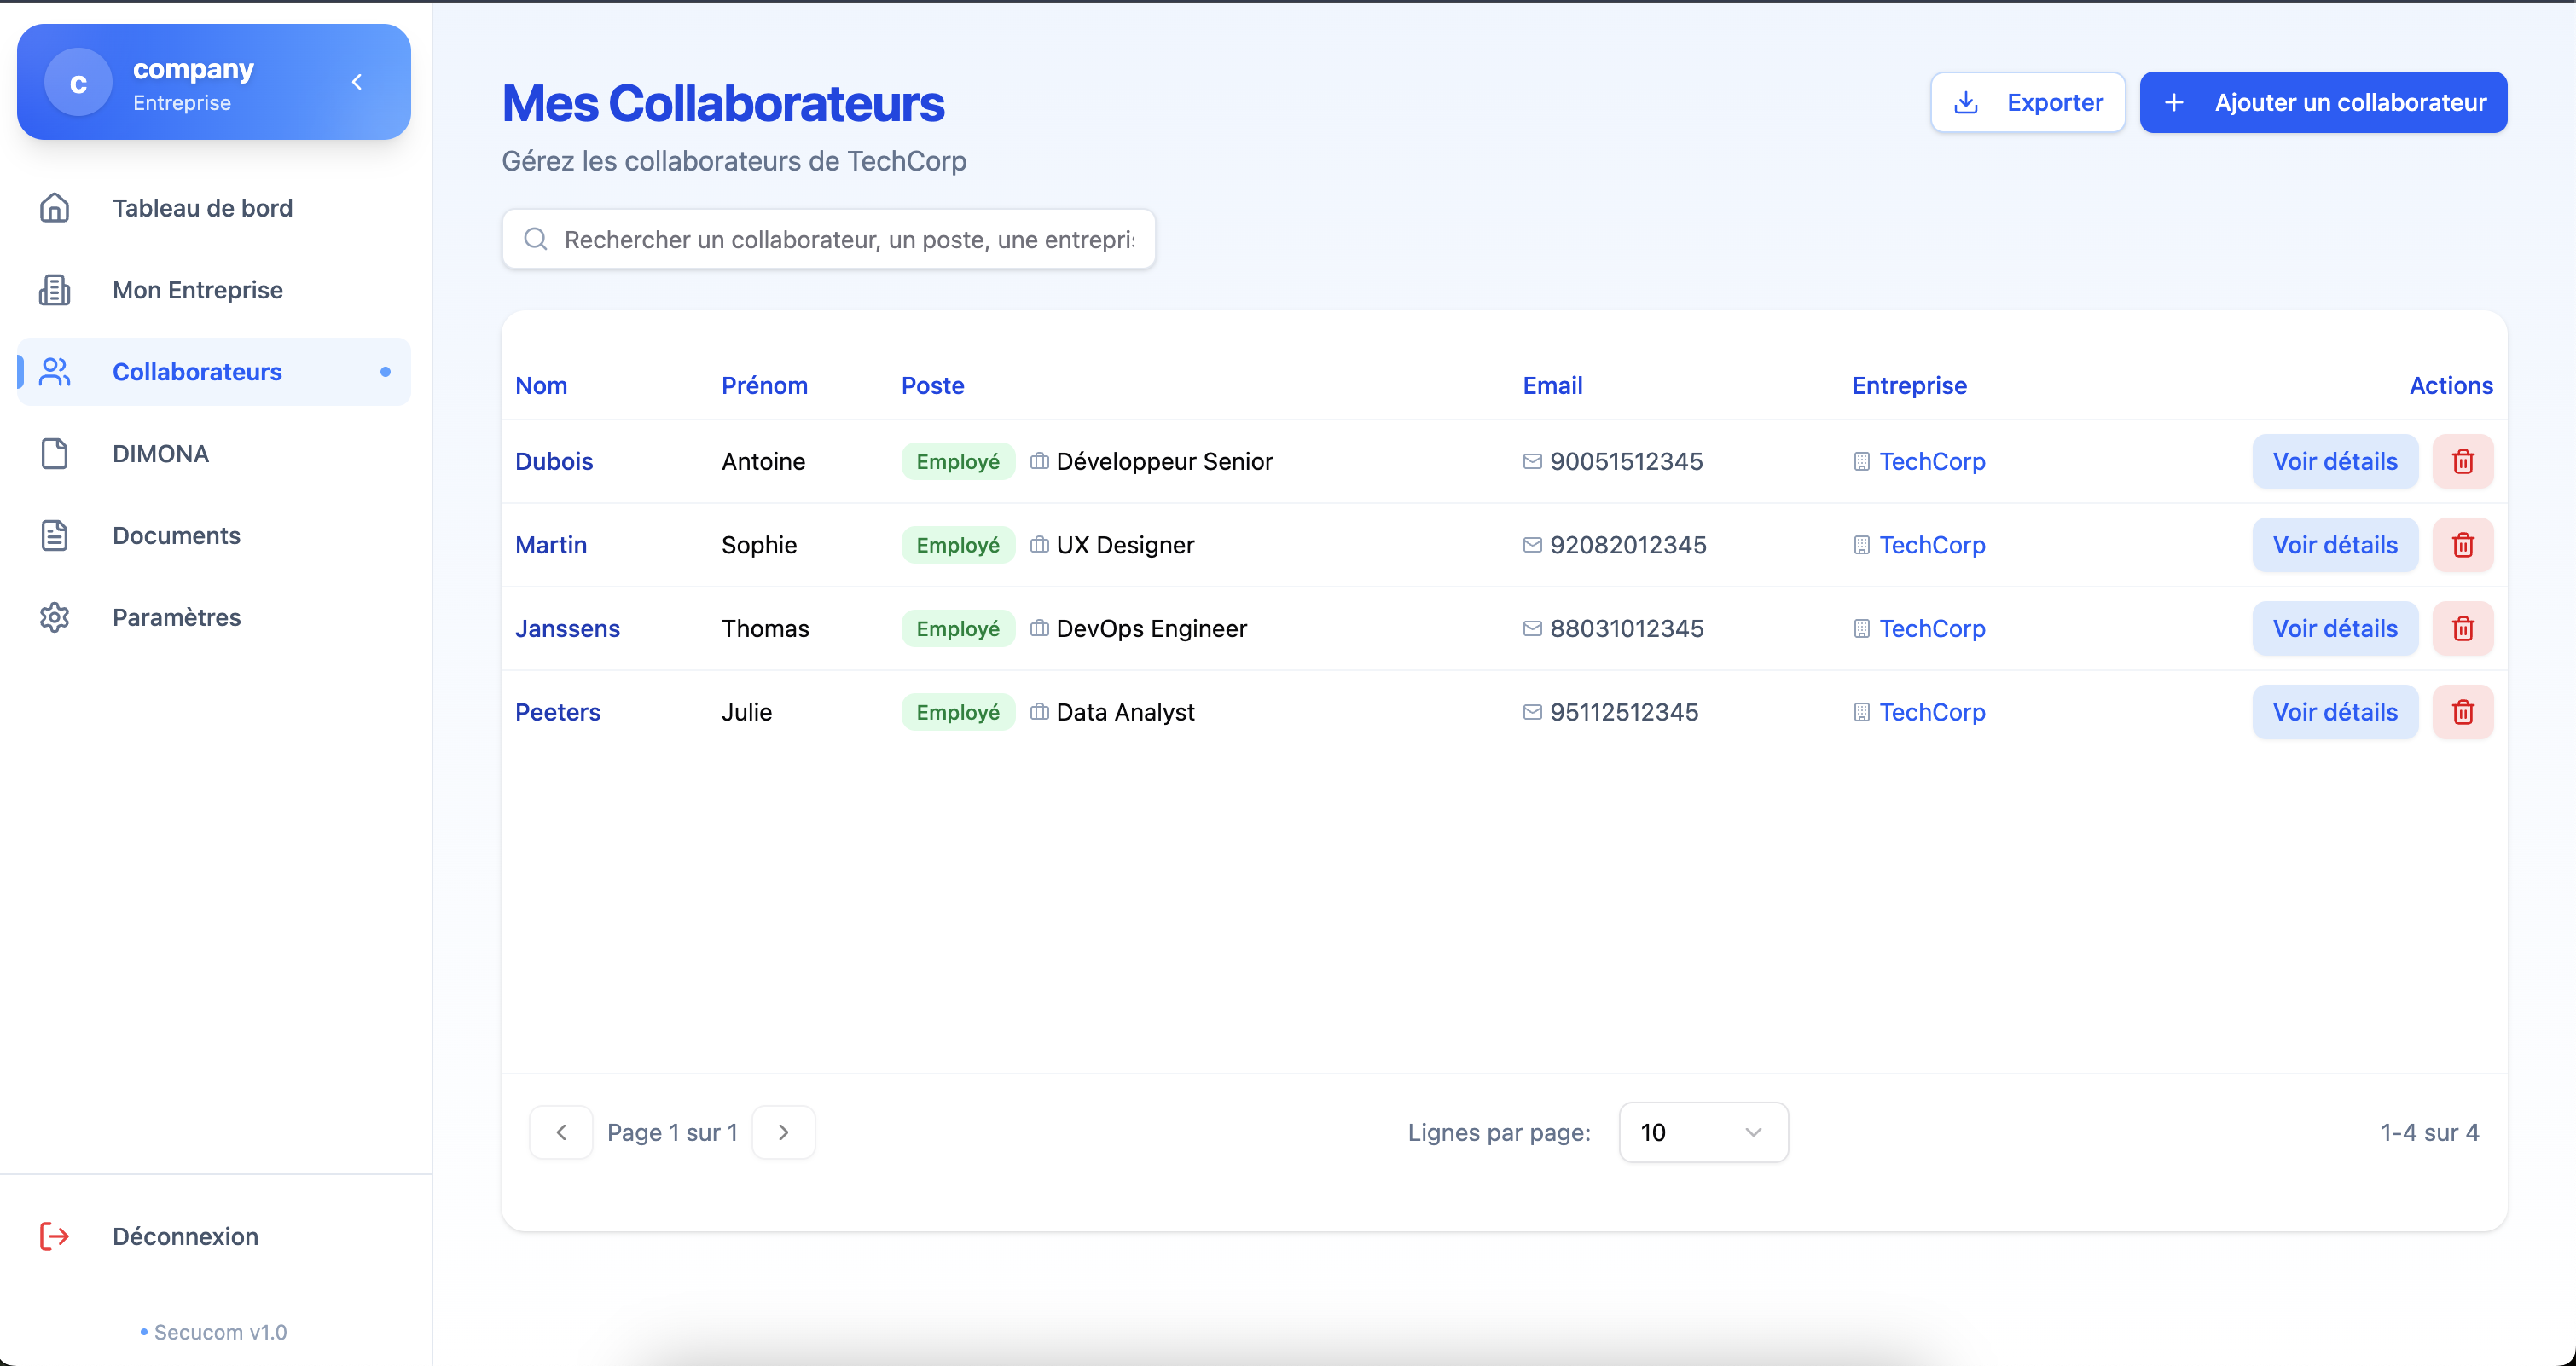
\includegraphics[width=1\textwidth]{SecuComPreviewCompanySpace.png}
  \caption{Aperçu de l'espace Entreprise}
  \label{fig:secucomPreviewUI}
\end{figure}

\vspace{0.5cm}

\begin{figure}[H]
  \centering
  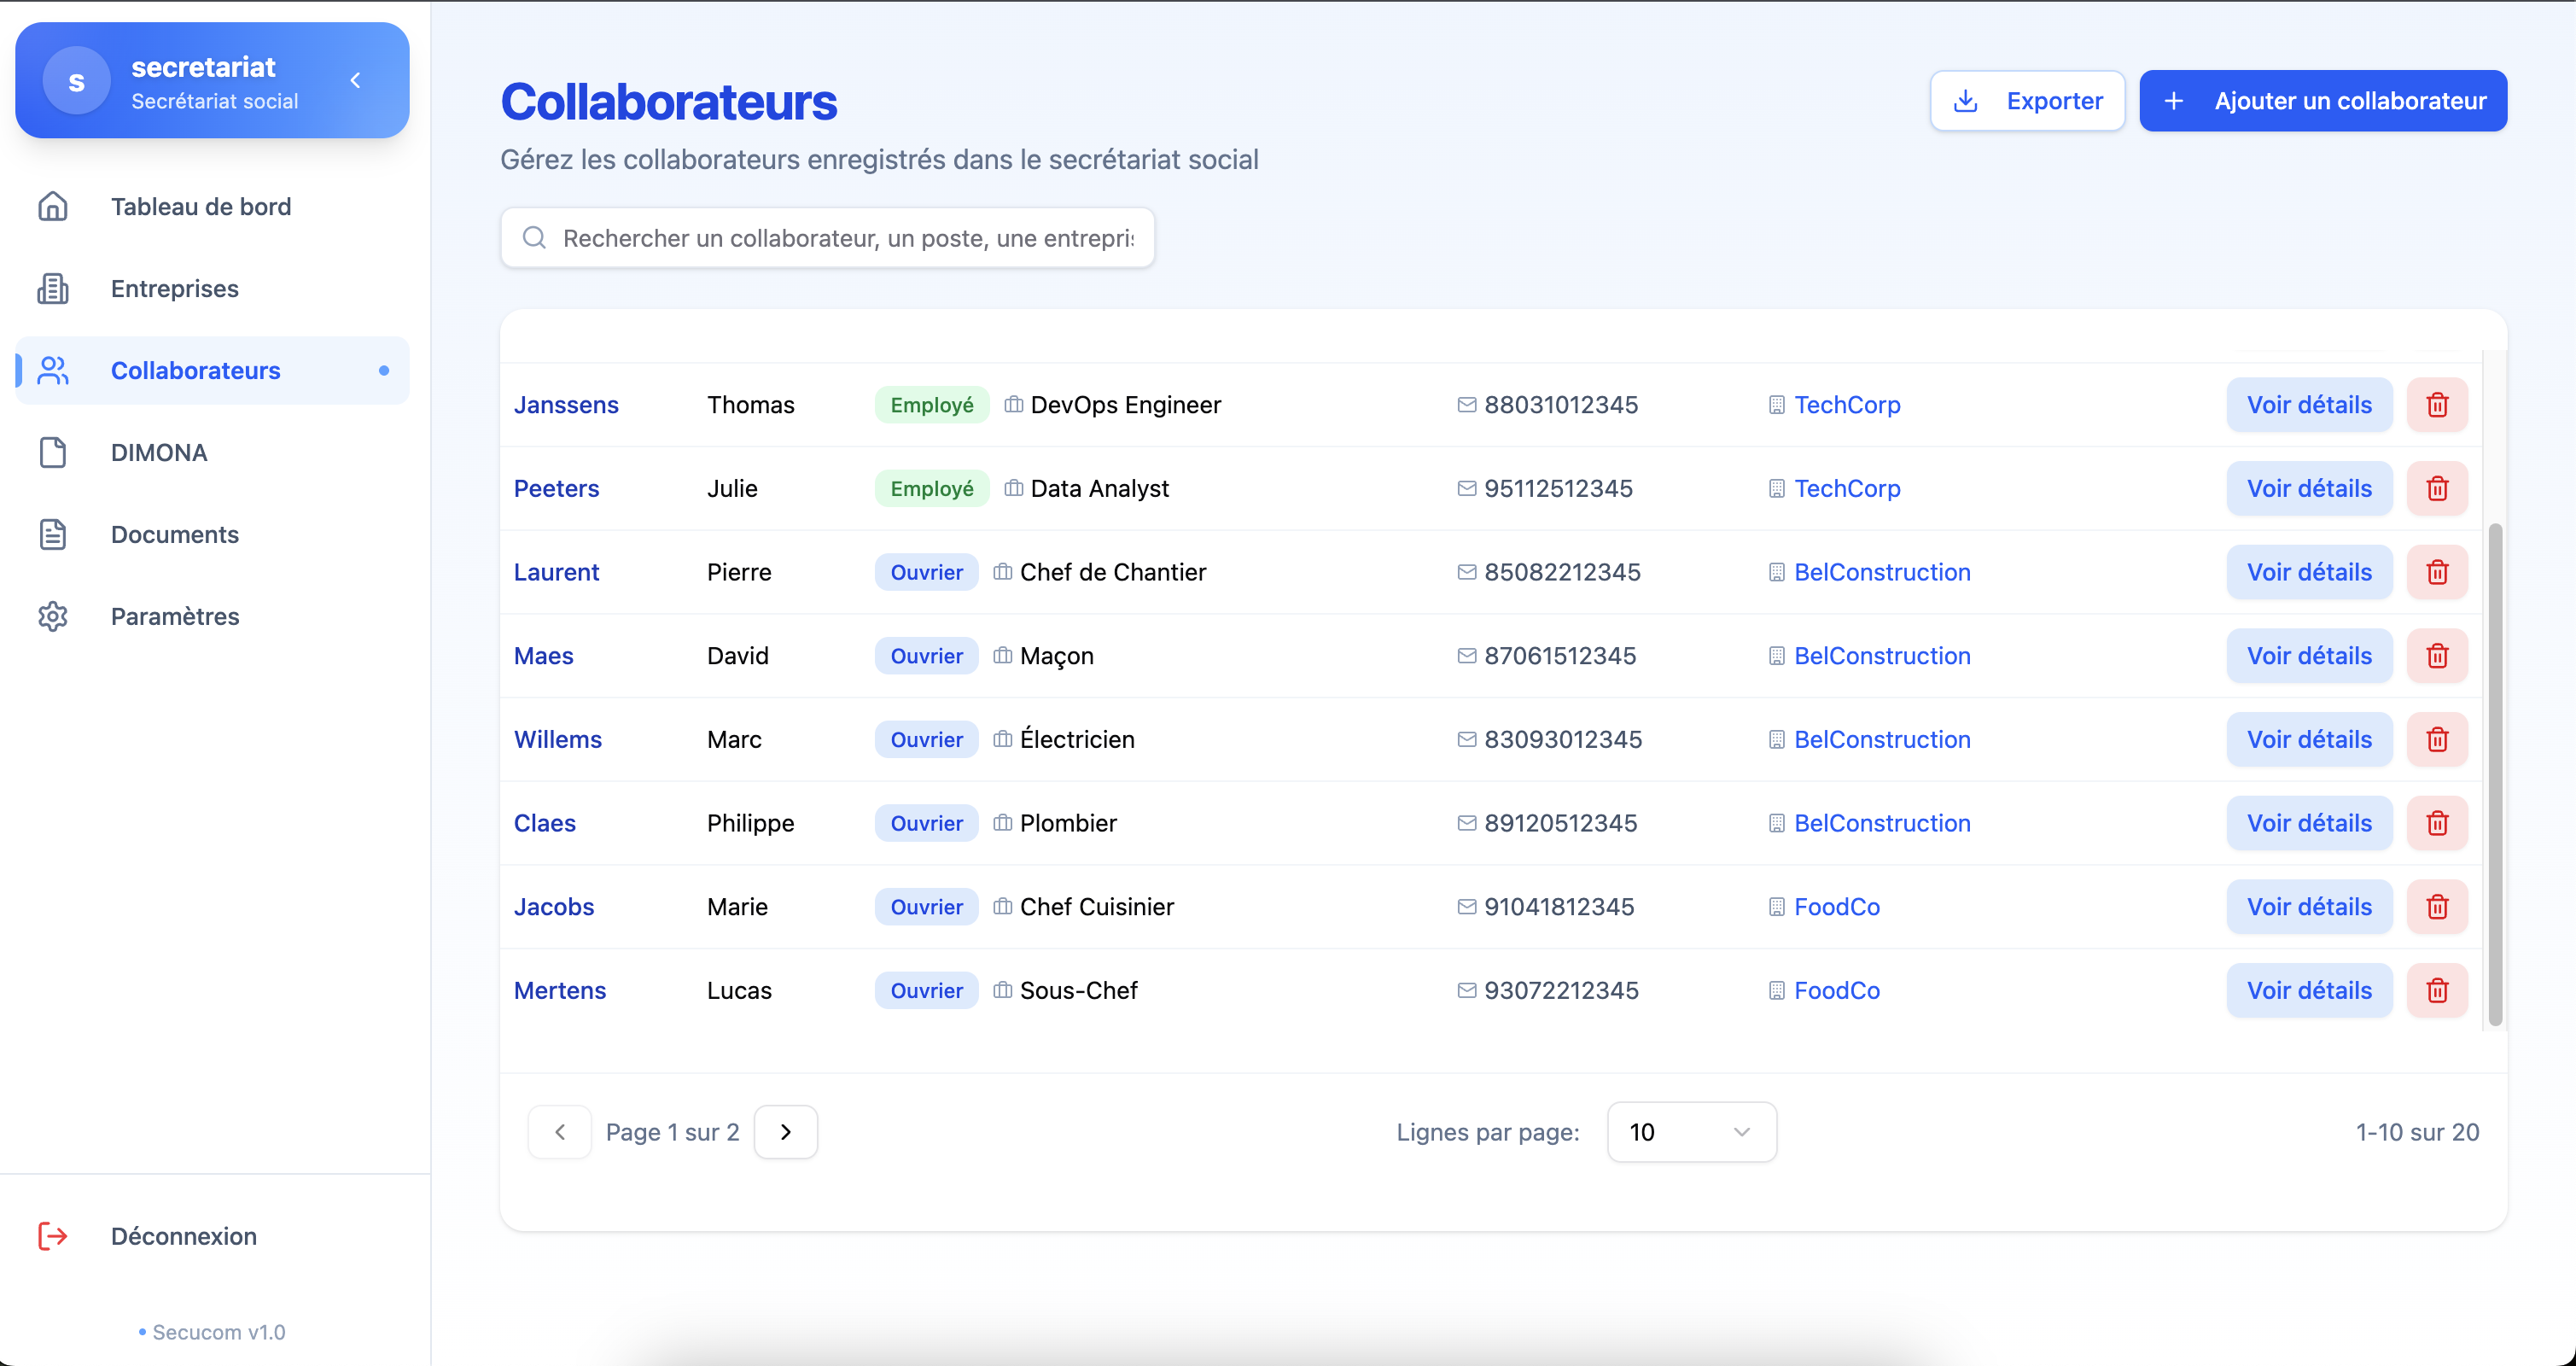
\includegraphics[width=1\textwidth]{SecuComPreviewSecretariatSpace.png}
  \caption{Aperçu de l'espace Secretariat social}
  \label{fig:secucomPreviewUI}
\end{figure}

\subsection{Modèles de données}

Les modèles de données constituent le cœur de l'application SecuCom. Ils représentent les entités métier et leurs relations, et sont implémentés sous forme de classes Java annotées avec JPA (Java Persistence API) pour la persistance en base de données.

\subsubsection{Entité User}

L'entité \texttt{User} représente la base de tous les utilisateurs du système. Elle utilise l'héritage avec une stratégie de table unique (\texttt{SINGLE\_TABLE}) pour différencier les types d'utilisateurs via une colonne discriminante.

\vspace{0.5cm}

\begin{figure}[H]
  \centering
  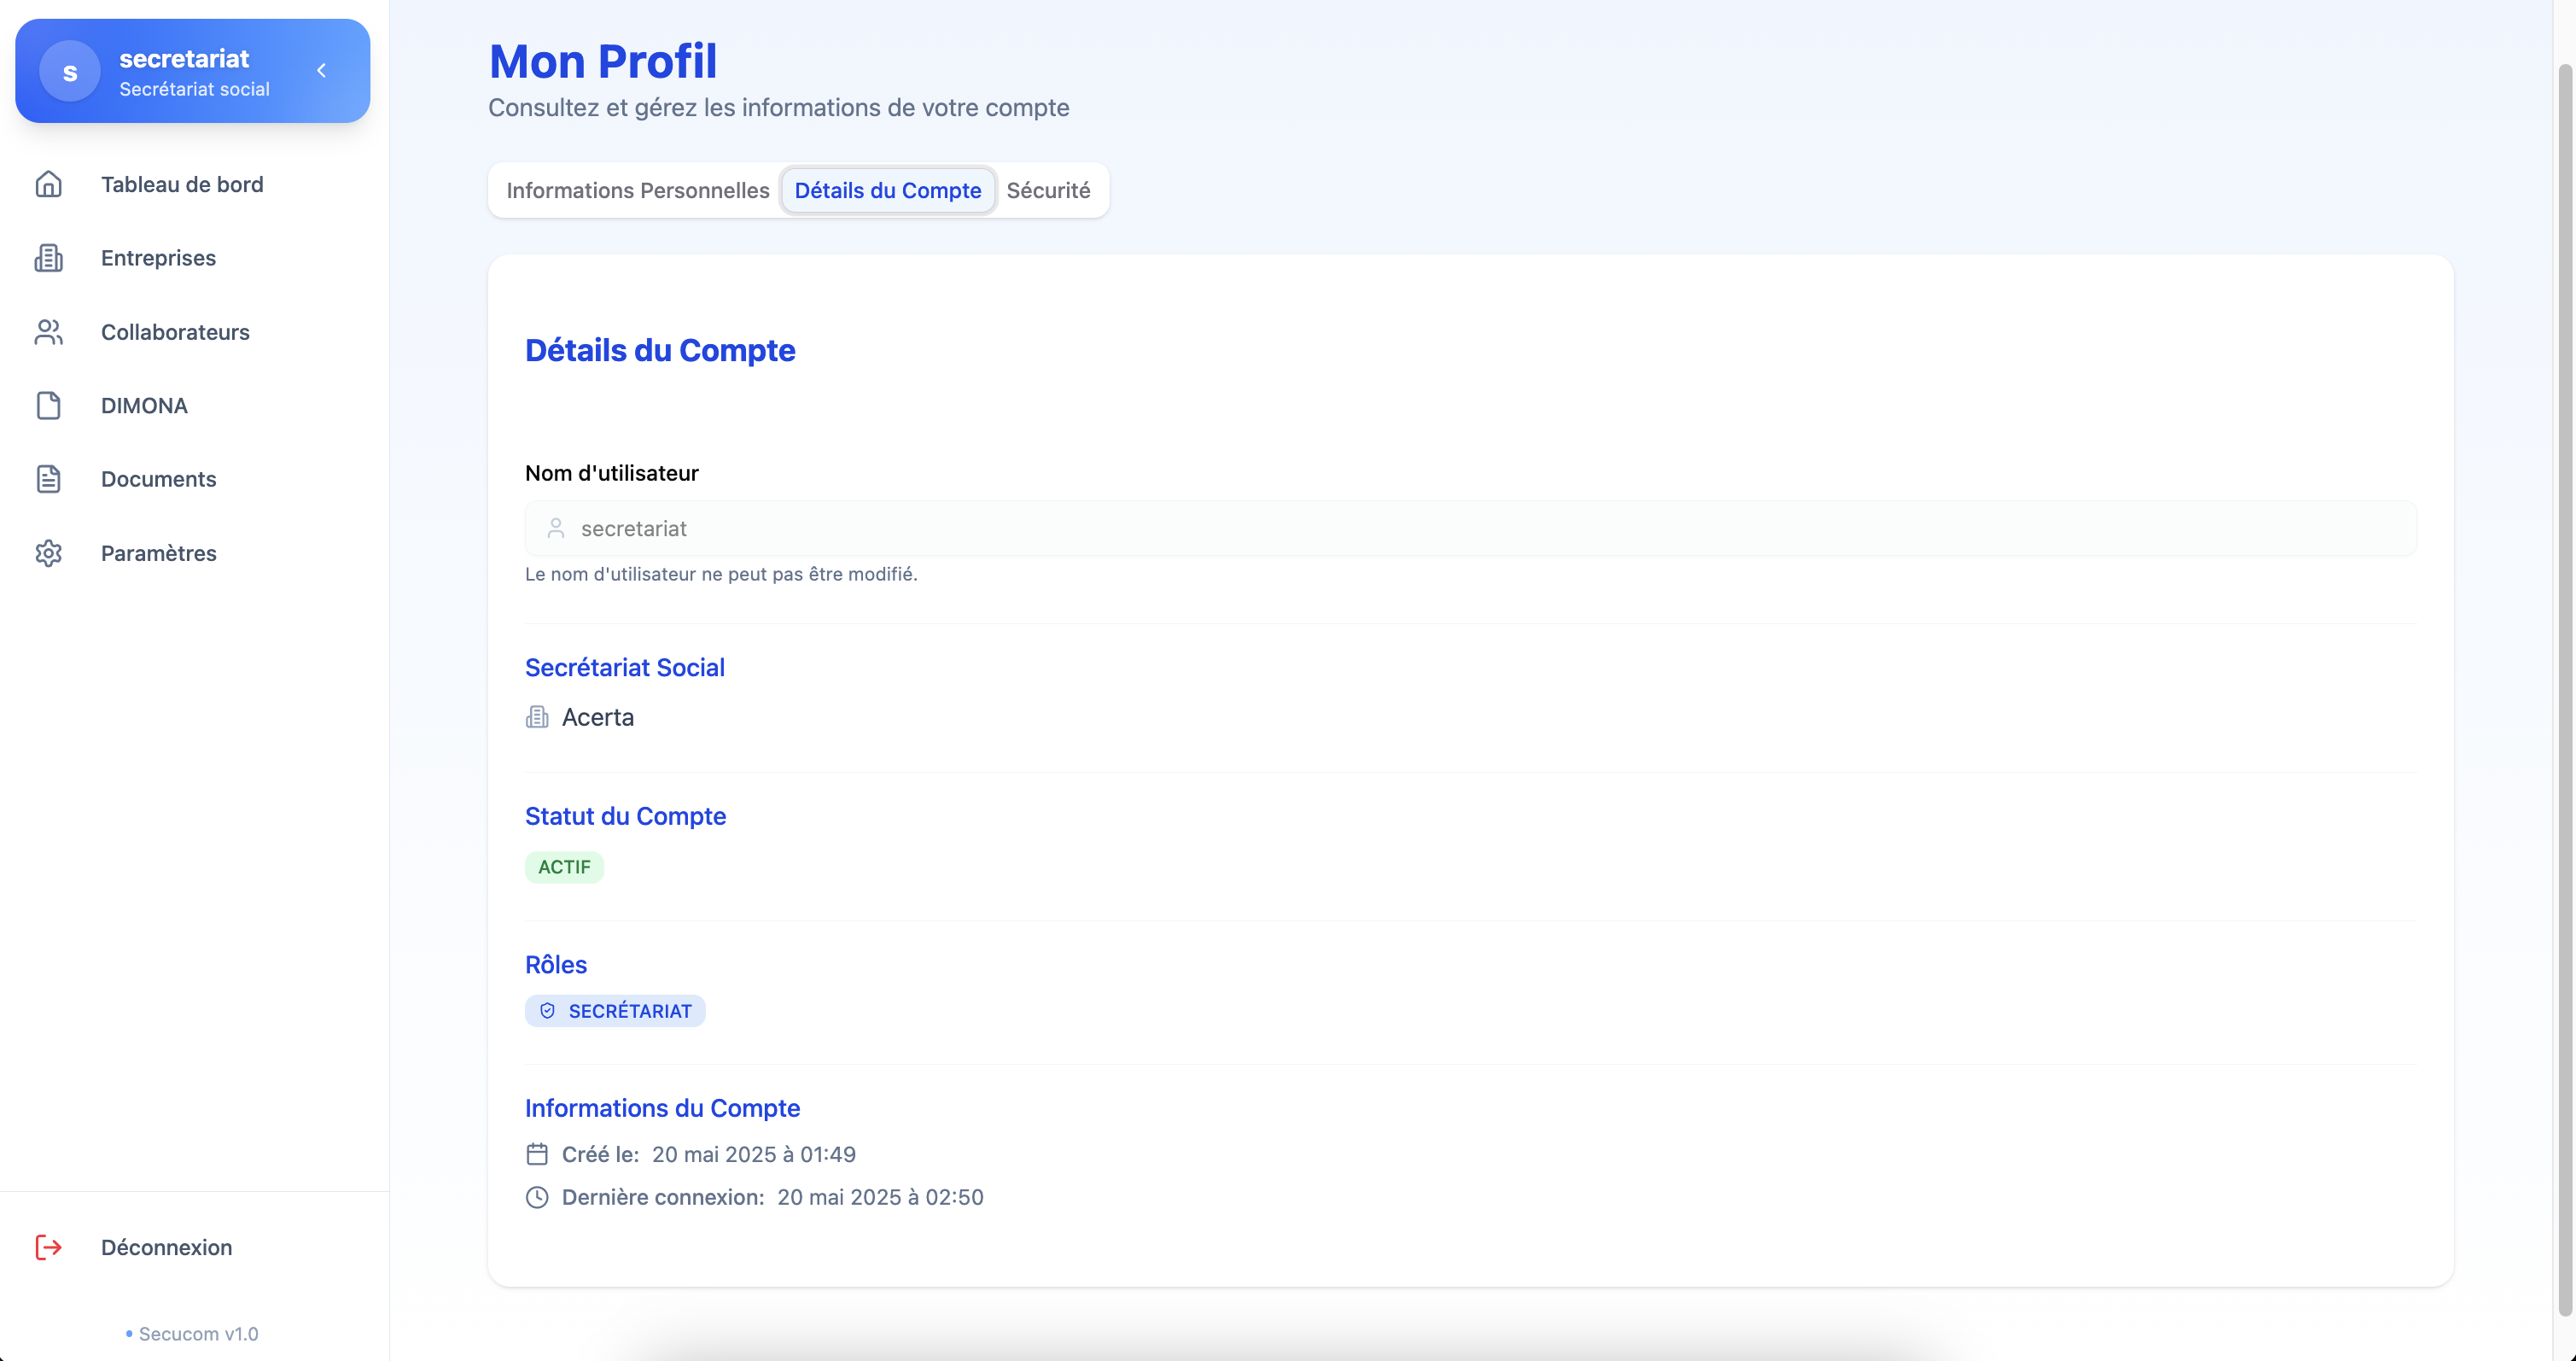
\includegraphics[width=1\textwidth]{SecuComPreviewUserProfile.png}
  \caption{Interface de gestion du profil utilisateur dans SecuCom}
  \label{fig:companyInterface}
\end{figure}

\vspace{0.5cm}

\begin{note}
Cette approche d'héritage permet de spécialiser les utilisateurs en différents types (employés du secrétariat, contacts d'entreprise) tout en maintenant une base commune pour l'authentification et les informations de base.
\end{note}

\subsubsection{Entité Company}

L'entité \texttt{Company} représente une entreprise cliente du secrétariat social. Elle contient de nombreux attributs reflétant les informations administratives et légales nécessaires.

\vspace{0.5cm}

\begin{figure}[H]
  \centering
  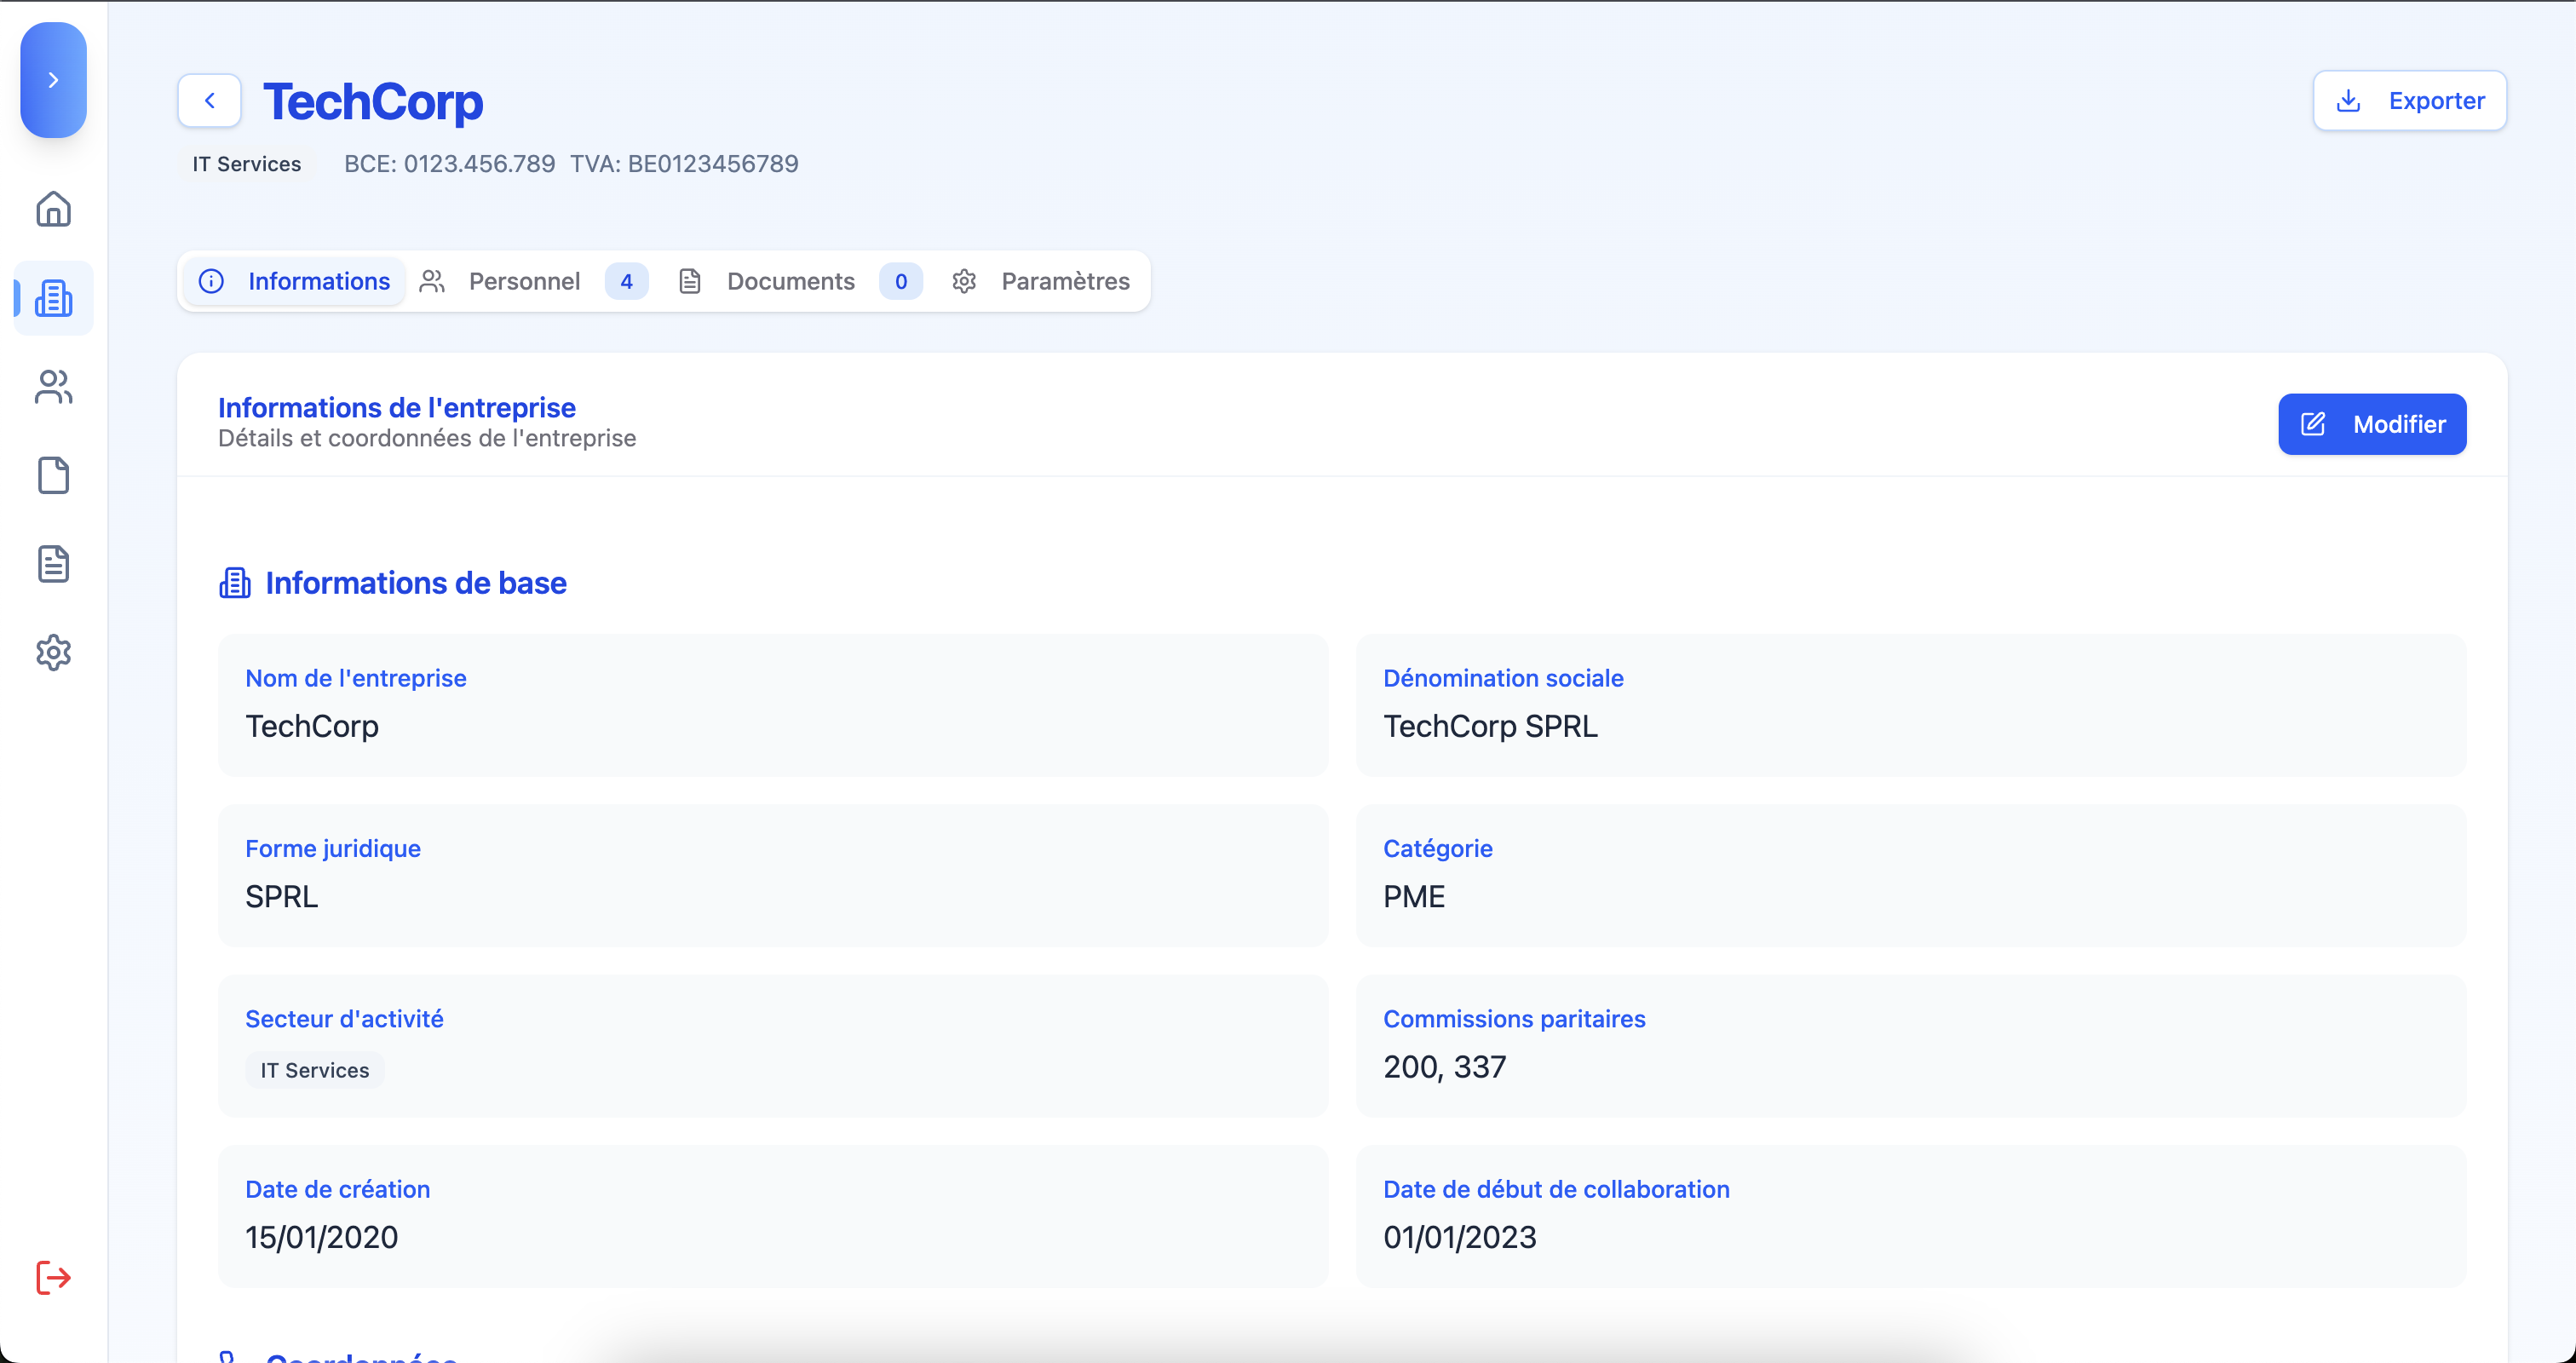
\includegraphics[width=1\textwidth]{SecuComPreviewCompany.png}
  \caption{Interface de gestion des entreprises dans SecuCom}
  \label{fig:companyInterface}
\end{figure}

\vspace{0.5cm}

Cette entité est au centre de nombreuses relations : elle est liée aux contacts d'entreprise, aux collaborateurs et aux déclarations DIMONA.

\subsubsection{Entité Collaborator}

L'entité \texttt{Collaborator} représente un travailleur d'une entreprise cliente. Elle contient des informations personnelles et professionnelles détaillées.

\vspace{0.5cm}

\begin{figure}[H]
  \centering
  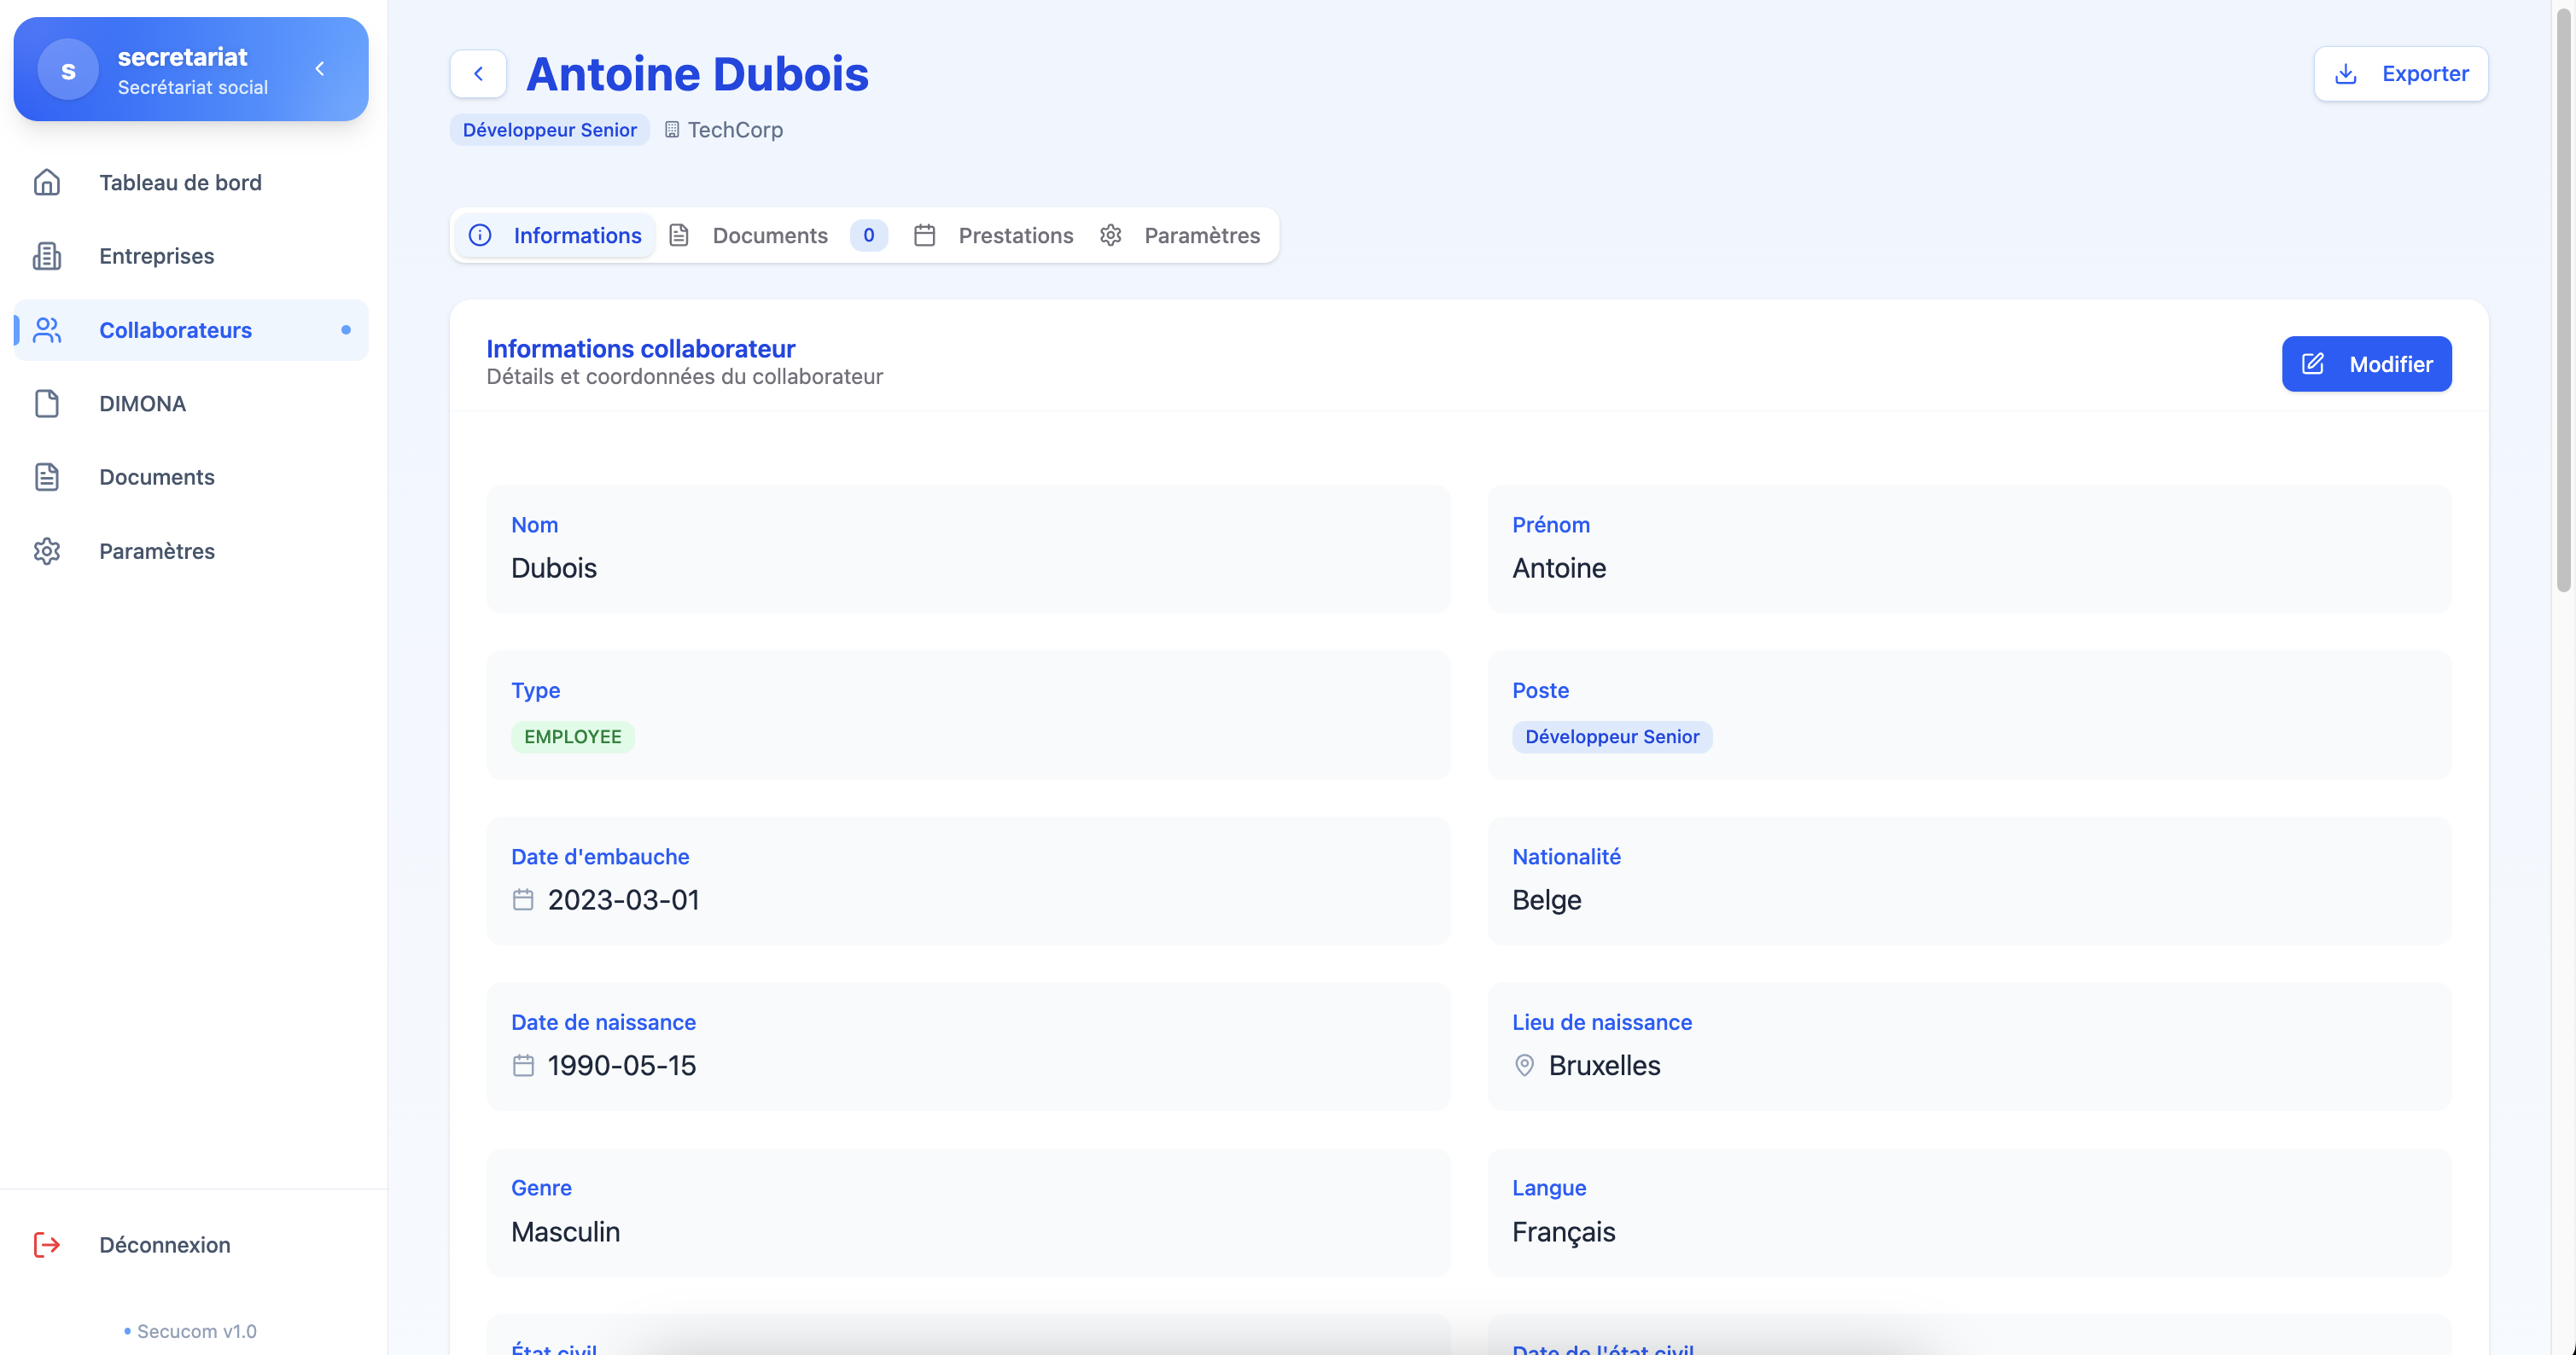
\includegraphics[width=1\textwidth]{SecuComPreviewCollaboratorInfos.png}
  \caption{Interface de gestion des collaborateurs dans SecuCom}
  \label{fig:collaboratorInterface}
\end{figure}

\vspace{0.5cm}

Cette entité utilise des types énumérés pour certains attributs comme le type de collaborateur (\texttt{EMPLOYEE}, \texttt{WORKER}, etc.) et le type de durée de travail (\texttt{FIXED}, \texttt{VARIABLE}).

\subsubsection{Entité Dimona}

L'entité \texttt{Dimona} représente une déclaration DIMONA associée à un collaborateur et à une entreprise.

\vspace{0.5cm}

\begin{figure}[H]
  \centering
  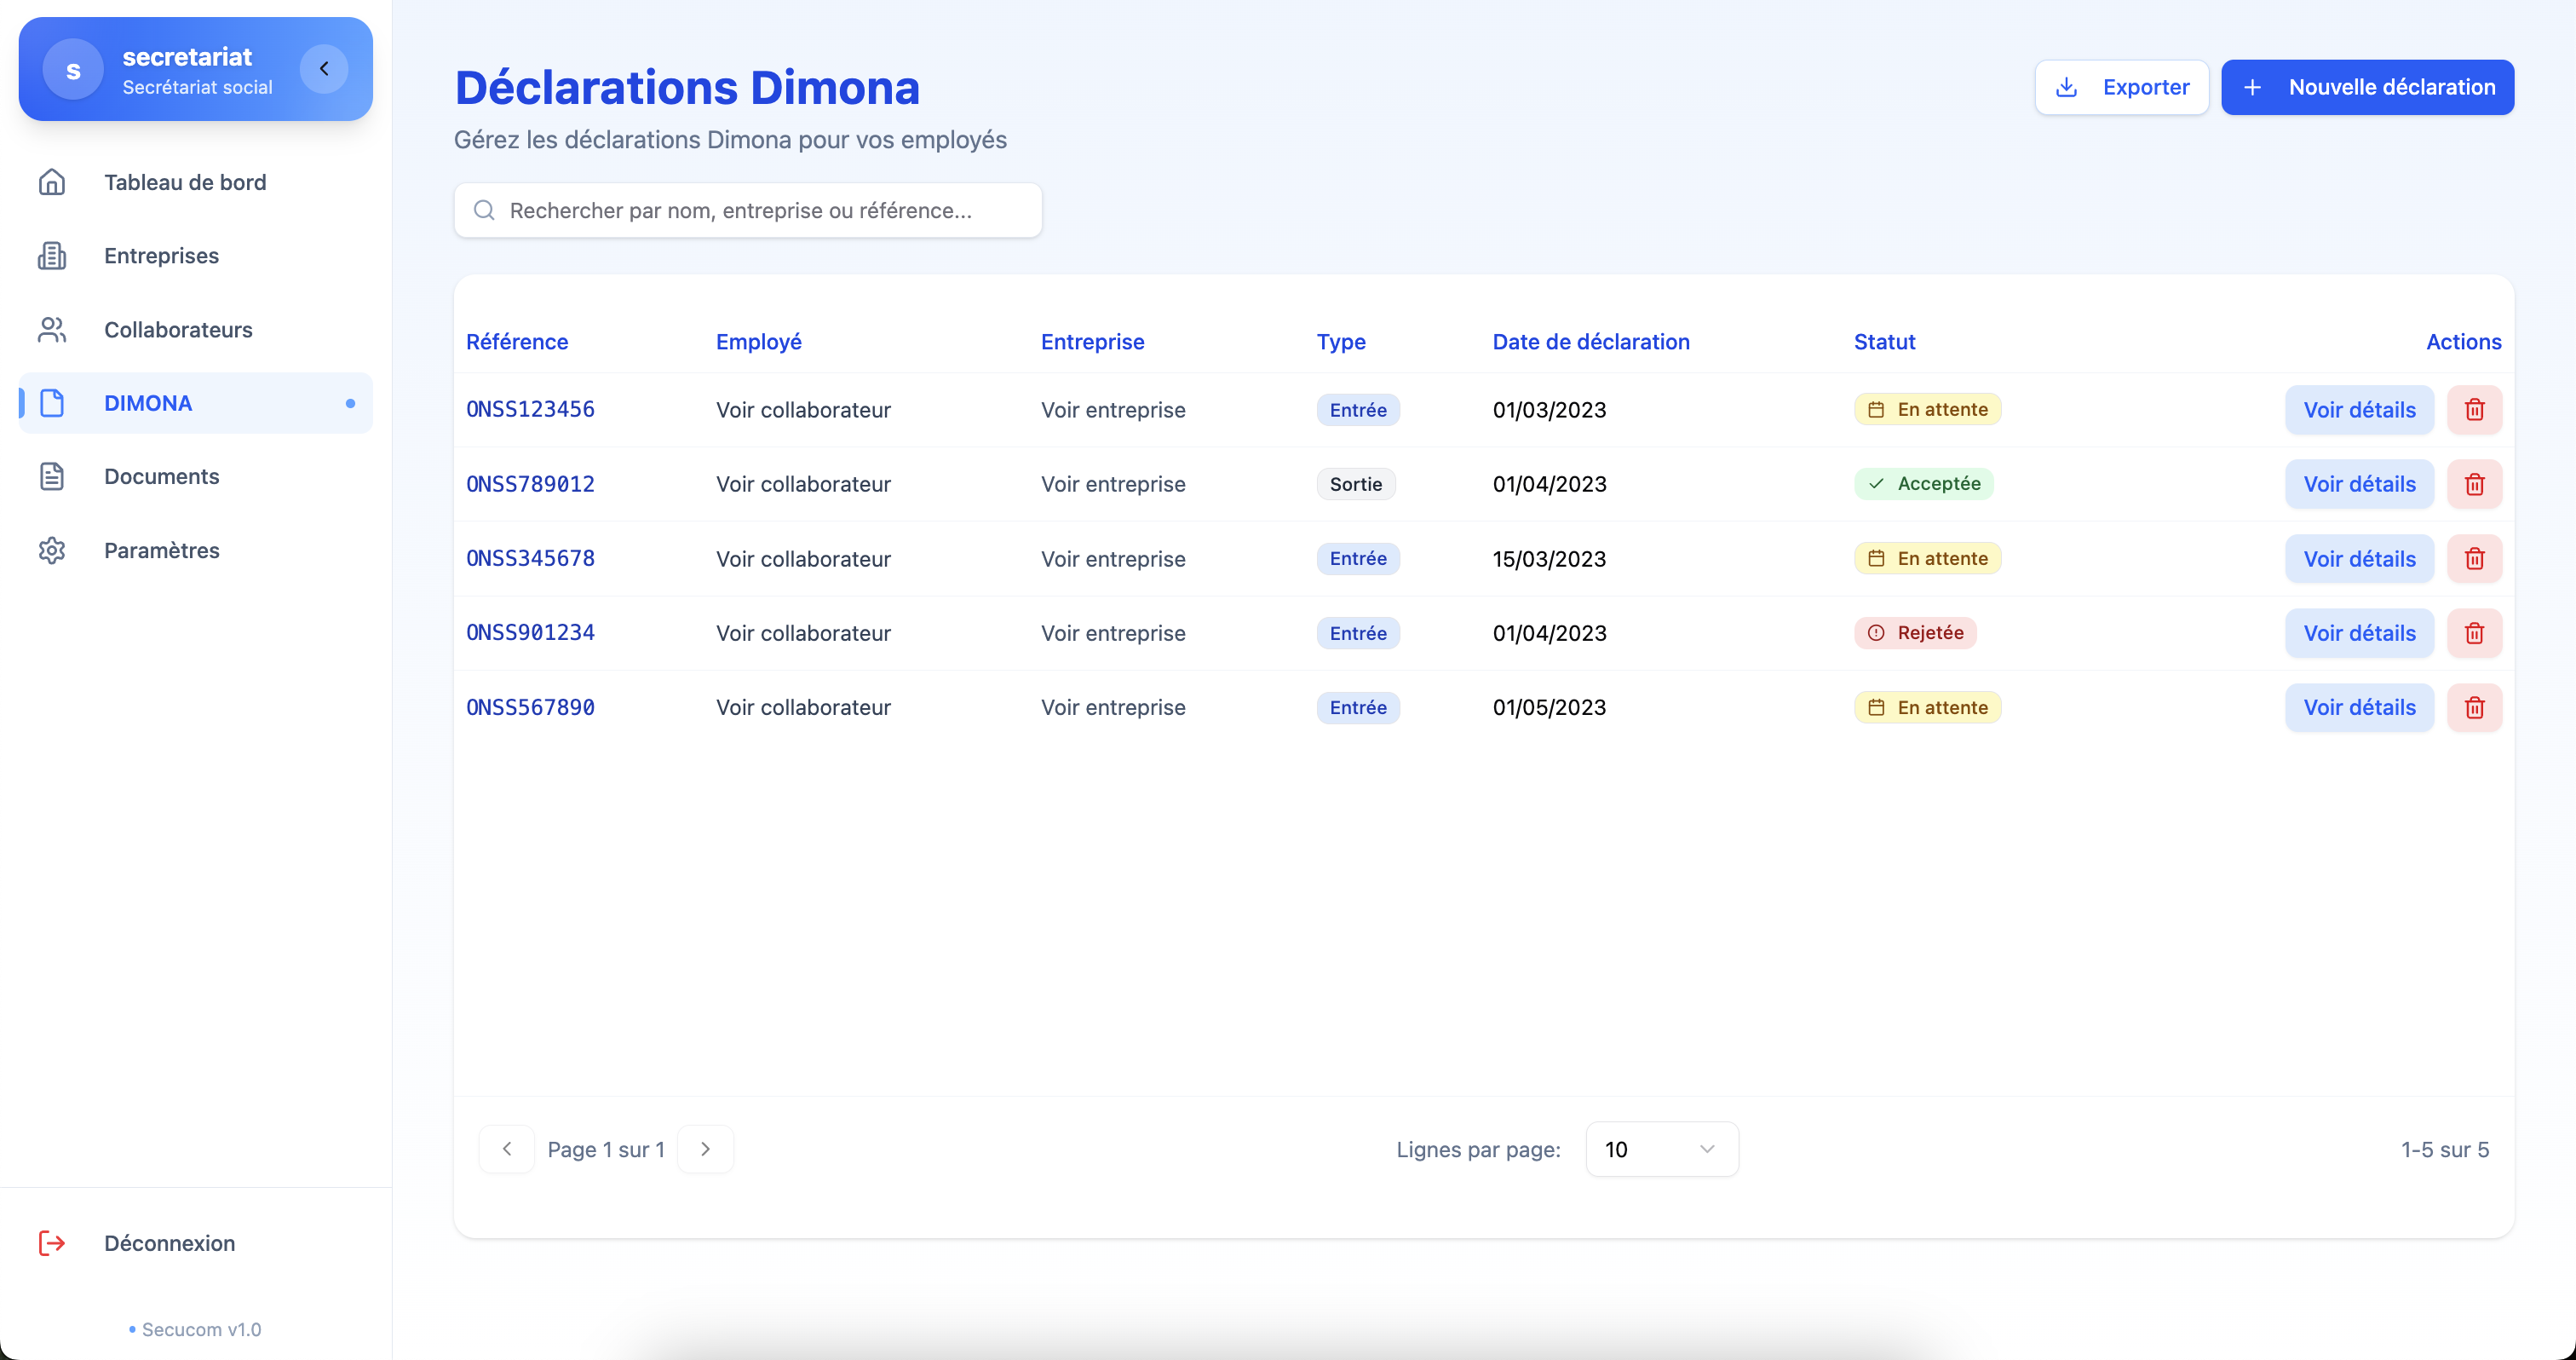
\includegraphics[width=1\textwidth]{SecuComPreviewDimona.png}
  \caption{Interface de gestion des dimonas dans SecuCom}
  \label{fig:companyInterface}
\end{figure}

\vspace{0.5cm}

Cette entité permet de suivre l'état des déclarations DIMONA et de conserver les références attribuées par l'ONSS.

\subsubsection{Autres entités et relations}

Le modèle de données comprend également d'autres entités comme \texttt{Address} (utilisée comme classe embarquée dans plusieurs entités), \texttt{SocialSecretariat} (représentant le secrétariat social) et \texttt{SecretariatEmployee} (représentant un employé du secrétariat social).

\vspace{0.5cm}

\noindent Les relations entre ces entités sont soigneusement définies pour refléter la réalité métier :
\begin{itemize}[leftmargin=*,label=\textcolor{darkgray}{$\bullet$},itemsep=0.3em]
  \item Une entreprise peut avoir plusieurs contacts et plusieurs collaborateurs (relations one-to-many).
  \item Un collaborateur appartient à une seule entreprise (relation many-to-one).
  \item Une déclaration DIMONA est associée à un collaborateur et à une entreprise (relations many-to-one).
  \item Un utilisateur peut avoir plusieurs rôles (relation one-to-many avec une collection d'énumérations).
\end{itemize}

\vspace{0.5cm}

\begin{tcolorbox}[
  title={\textbf{Modélisation des données}},
  colback=blue!5!white,
  colframe=primarycolor,
  fonttitle=\bfseries,
  boxrule=0.5mm,
  arc=2mm,
  left=6mm,
  right=6mm,
  top=6mm,
  bottom=6mm
]
Cette modélisation riche permet de représenter fidèlement les concepts métier tout en facilitant les requêtes et les manipulations de données. L'utilisation de JPA et Hibernate offre une abstraction puissante qui simplifie considérablement le code d'accès aux données.
\end{tcolorbox}

\subsection{Contrôleurs et services}

L'architecture de SecuCom s'appuie sur une séparation claire entre les contrôleurs, qui exposent les API REST, et les services, qui implémentent la logique métier. Cette séparation permet une meilleure organisation du code et facilite les tests.

\subsubsection{Contrôleurs REST}

Les contrôleurs REST sont responsables de la gestion des requêtes HTTP, de la validation des données d'entrée et de la transformation des réponses. Ils sont annotés avec \texttt{@RestController} et définissent des endpoints accessibles via des methodes HTTP (GET, POST, PUT, DELETE).

\vspace{0.5cm}

\begin{table}[H]
\centering
\begin{tabular}{|l|p{10cm}|}
\hline
\textbf{Contrôleur} & \textbf{Responsabilité} \\
\hline
AuthController & Gestion de l'authentification et des tokens JWT \\
\hline
CompanyController & Opérations CRUD sur les entreprises \\
\hline
CollaboratorController & Opérations CRUD sur les collaborateurs \\
\hline
DimonaController & Opérations liées aux déclarations DIMONA \\
\hline
UserController & Opérations sur les utilisateurs \\
\hline
SocialSecretariatController & Opérations liées au secrétariat social \\
\hline
\end{tabular}
\caption{Principaux contrôleurs de SecuCom}
\end{table}

\vspace{0.5cm}

Les contrôleurs utilisent des objets DTO (Data Transfer Object) pour les échanges avec les clients, ce qui permet de découpler les modèles internes des représentations externes.

\subsubsection{Services métier}

Les services métier encapsulent la logique fonctionnelle de l'application. Ils orchestrent les opérations entre les repositories et les contrôleurs, appliquent les règles métier et gèrent les transactions.

\vspace{0.5cm}

\begin{note}
Les services utilisent l'annotation \texttt{@Transactional} pour gérer les transactions de manière déclarative, assurant l'intégrité des données même en cas d'erreur.
\end{note}

\newpage

\noindent Les principaux services de l'application sont :
\begin{itemize}[leftmargin=*,label=\textcolor{darkgray}{$\bullet$},itemsep=0.3em]
  \item \texttt{AuthService} : Gère l'authentification et la génération des tokens.
  \item \texttt{CompanyService} : Implémente la logique métier pour les entreprises.
  \item \texttt{CollaboratorService} : Implémente la logique métier pour les collaborateurs.
  \item \texttt{DimonaService} : Implémente la logique métier pour les déclarations DIMONA.
  \item \texttt{UserService} : Implémente la logique métier pour les utilisateurs.
  \item \texttt{SocialSecretariatService} : Implémente la logique métier pour le secrétariat social.
\end{itemize}

\subsubsection{Repositories}

Les repositories fournissent une abstraction de l'accès aux données. Ils sont implémentés en utilisant Spring Data JPA, qui génère automatiquement les implémentations à partir d'interfaces.

\vspace{0.5cm}

\begin{tcolorbox}[
  title={\textbf{Avantages des repositories Spring Data}},
  colback=blue!5!white,
  colframe=primarycolor,
  fonttitle=\bfseries,
  boxrule=0.5mm,
  arc=2mm,
  left=6mm,
  right=6mm,
  top=6mm,
  bottom=6mm
]
Cette approche permet de réduire considérablement le code boilerplate tout en offrant des fonctionnalités puissantes comme le filtrage, le tri et la pagination. Les développeurs peuvent se concentrer sur la logique métier plutôt que sur les détails techniques de l'accès aux données.
\end{tcolorbox}

\subsubsection{DTOs (Data Transfer Objects)}

Les DTOs sont utilisés pour découpler les modèles internes des représentations externes. Ils permettent de :
\begin{itemize}[leftmargin=*,label=\textcolor{darkgray}{$\bullet$},itemsep=0.3em]
  \item Contrôler précisément les données exposées aux clients
  \item Valider les données d'entrée indépendamment des entités
  \item Adapter le format des données aux besoins spécifiques des clients
\end{itemize}

\vspace{0.5cm}

La conversion entre DTOs et entités est généralement gérée par des bibliothèques comme ModelMapper ou MapStruct, ou par des methodes de conversion manuelles dans les services.

\section{Fonctionnalités principales}

\subsection{Gestion des entreprises}

La gestion des entreprises est une fonctionnalité centrale de SecuCom, permettant au secrétariat social de gérer efficacement ses clients. Cette fonctionnalité est implémentée à travers plusieurs composants qui travaillent ensemble.

\vspace{0.5cm}

\begin{figure}[H]
  \centering
  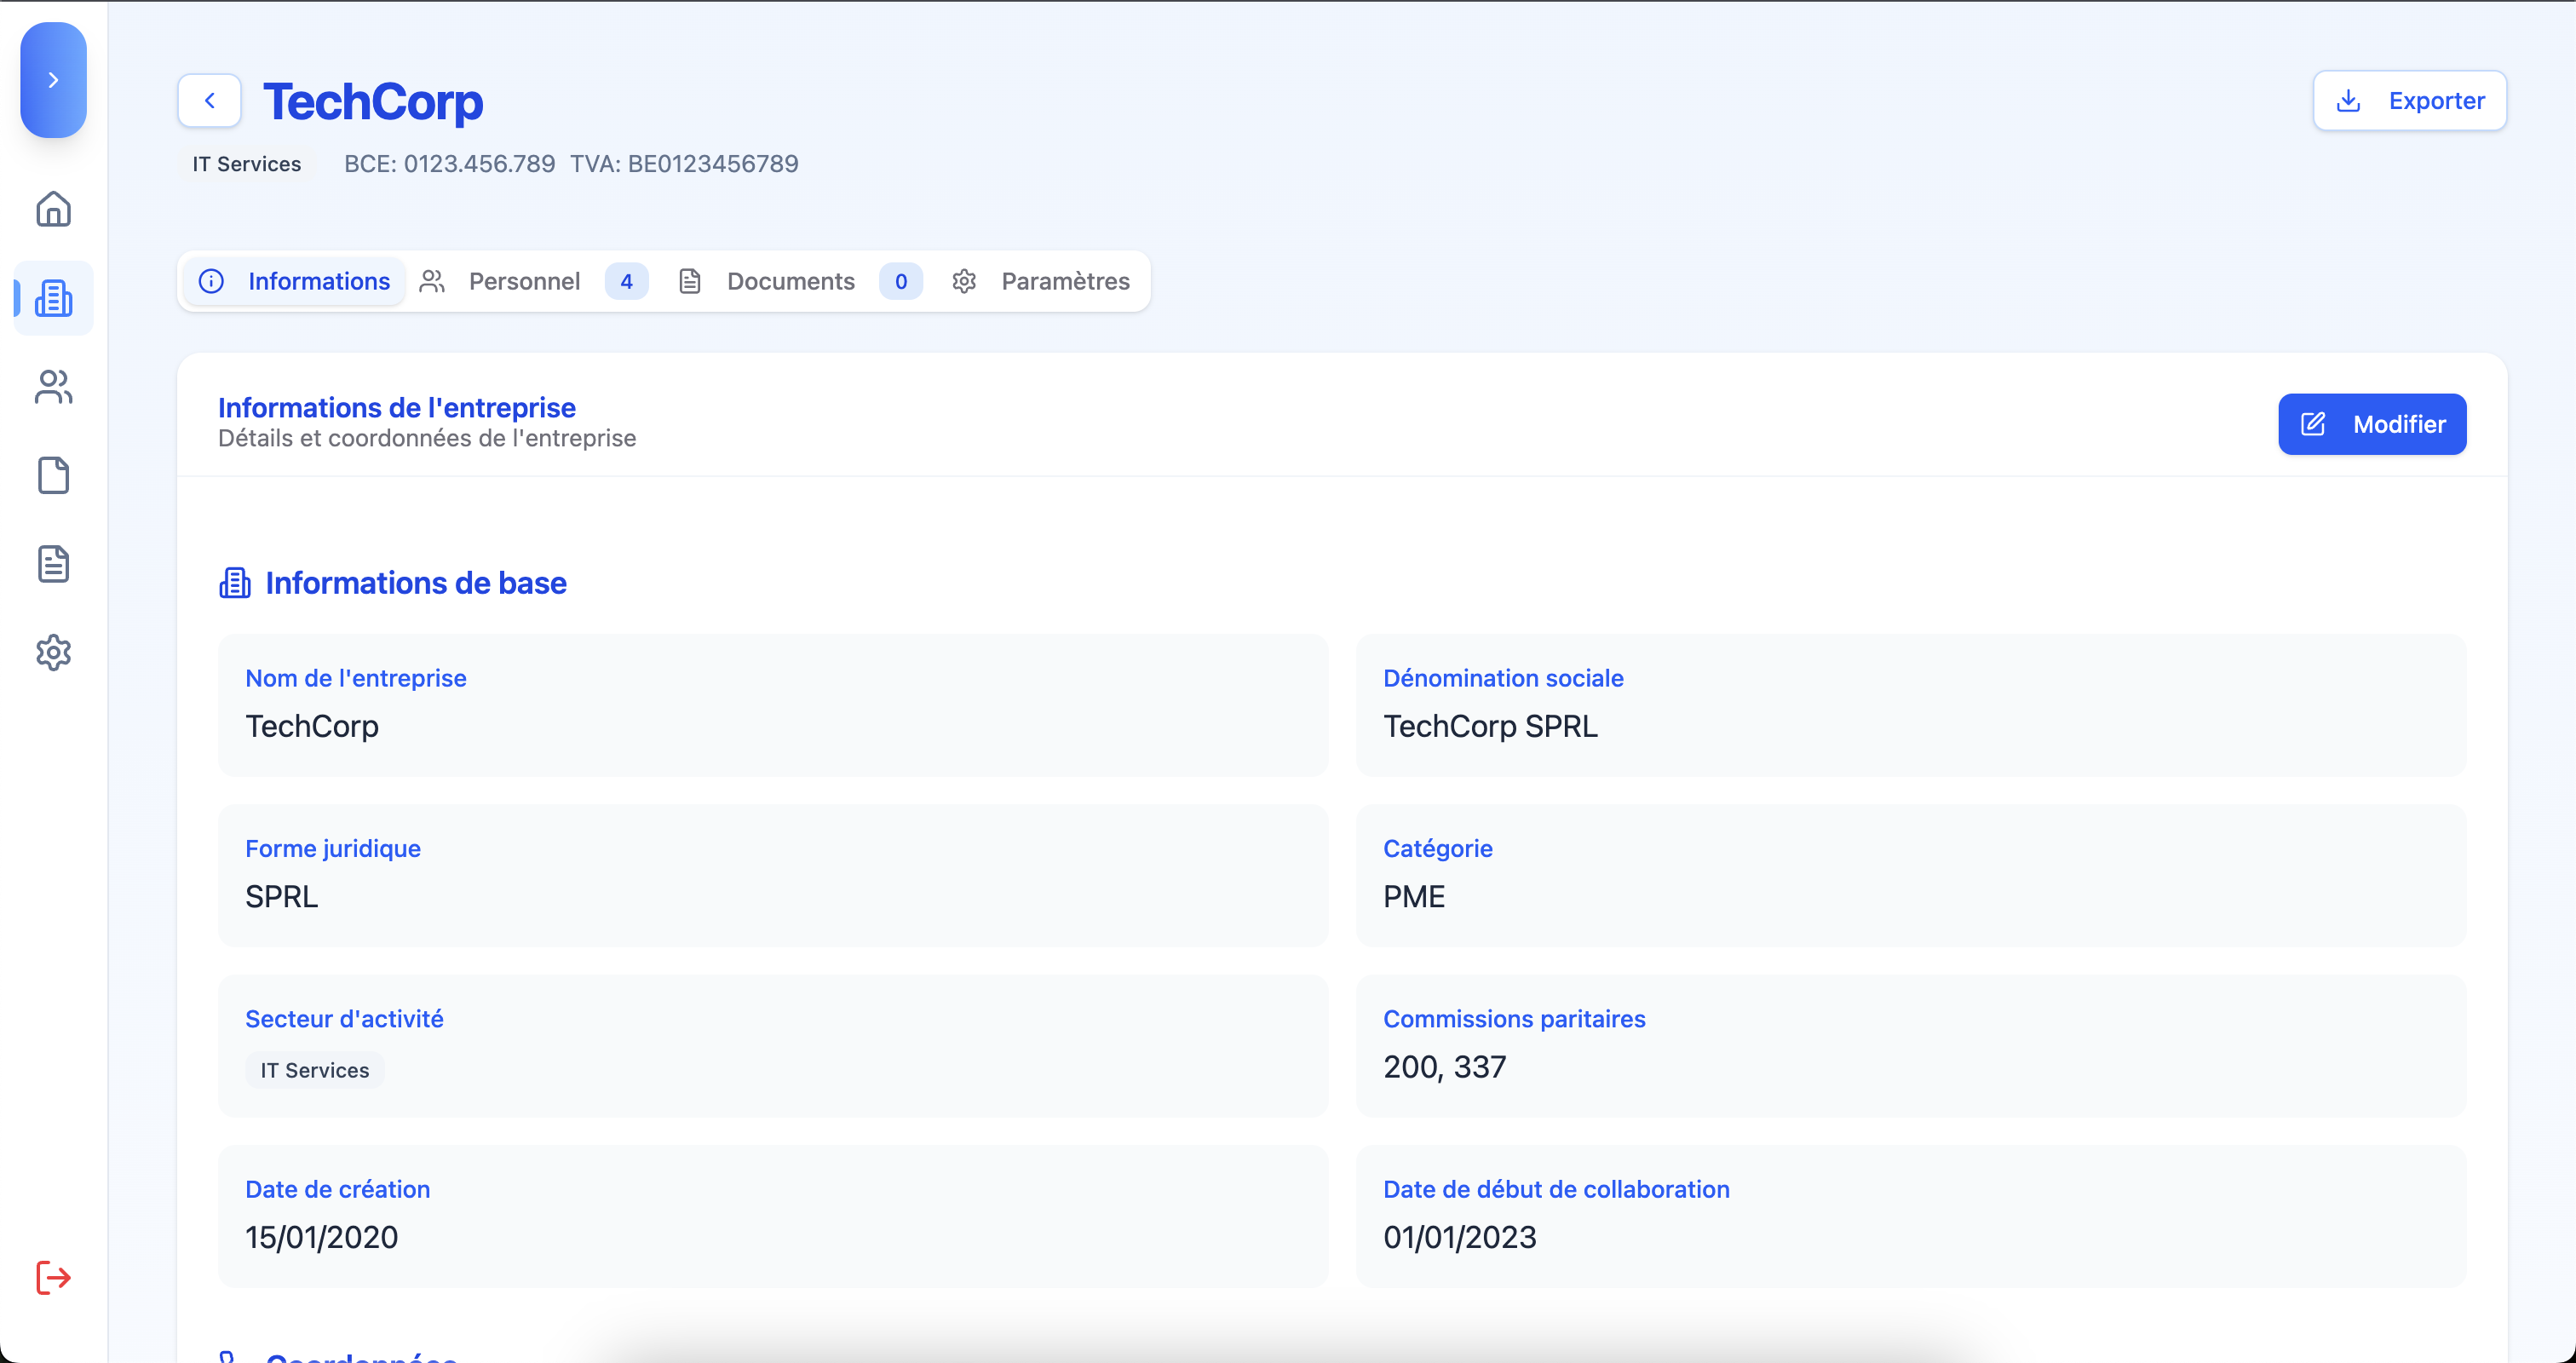
\includegraphics[width=1\textwidth]{SecuComPreviewCompany.png}
  \caption{Interface de gestion des entreprises dans SecuCom}
  \label{fig:companyManagementInterface}
\end{figure}
\vspace{0.5cm}
\begin{figure}[H]
  \centering
  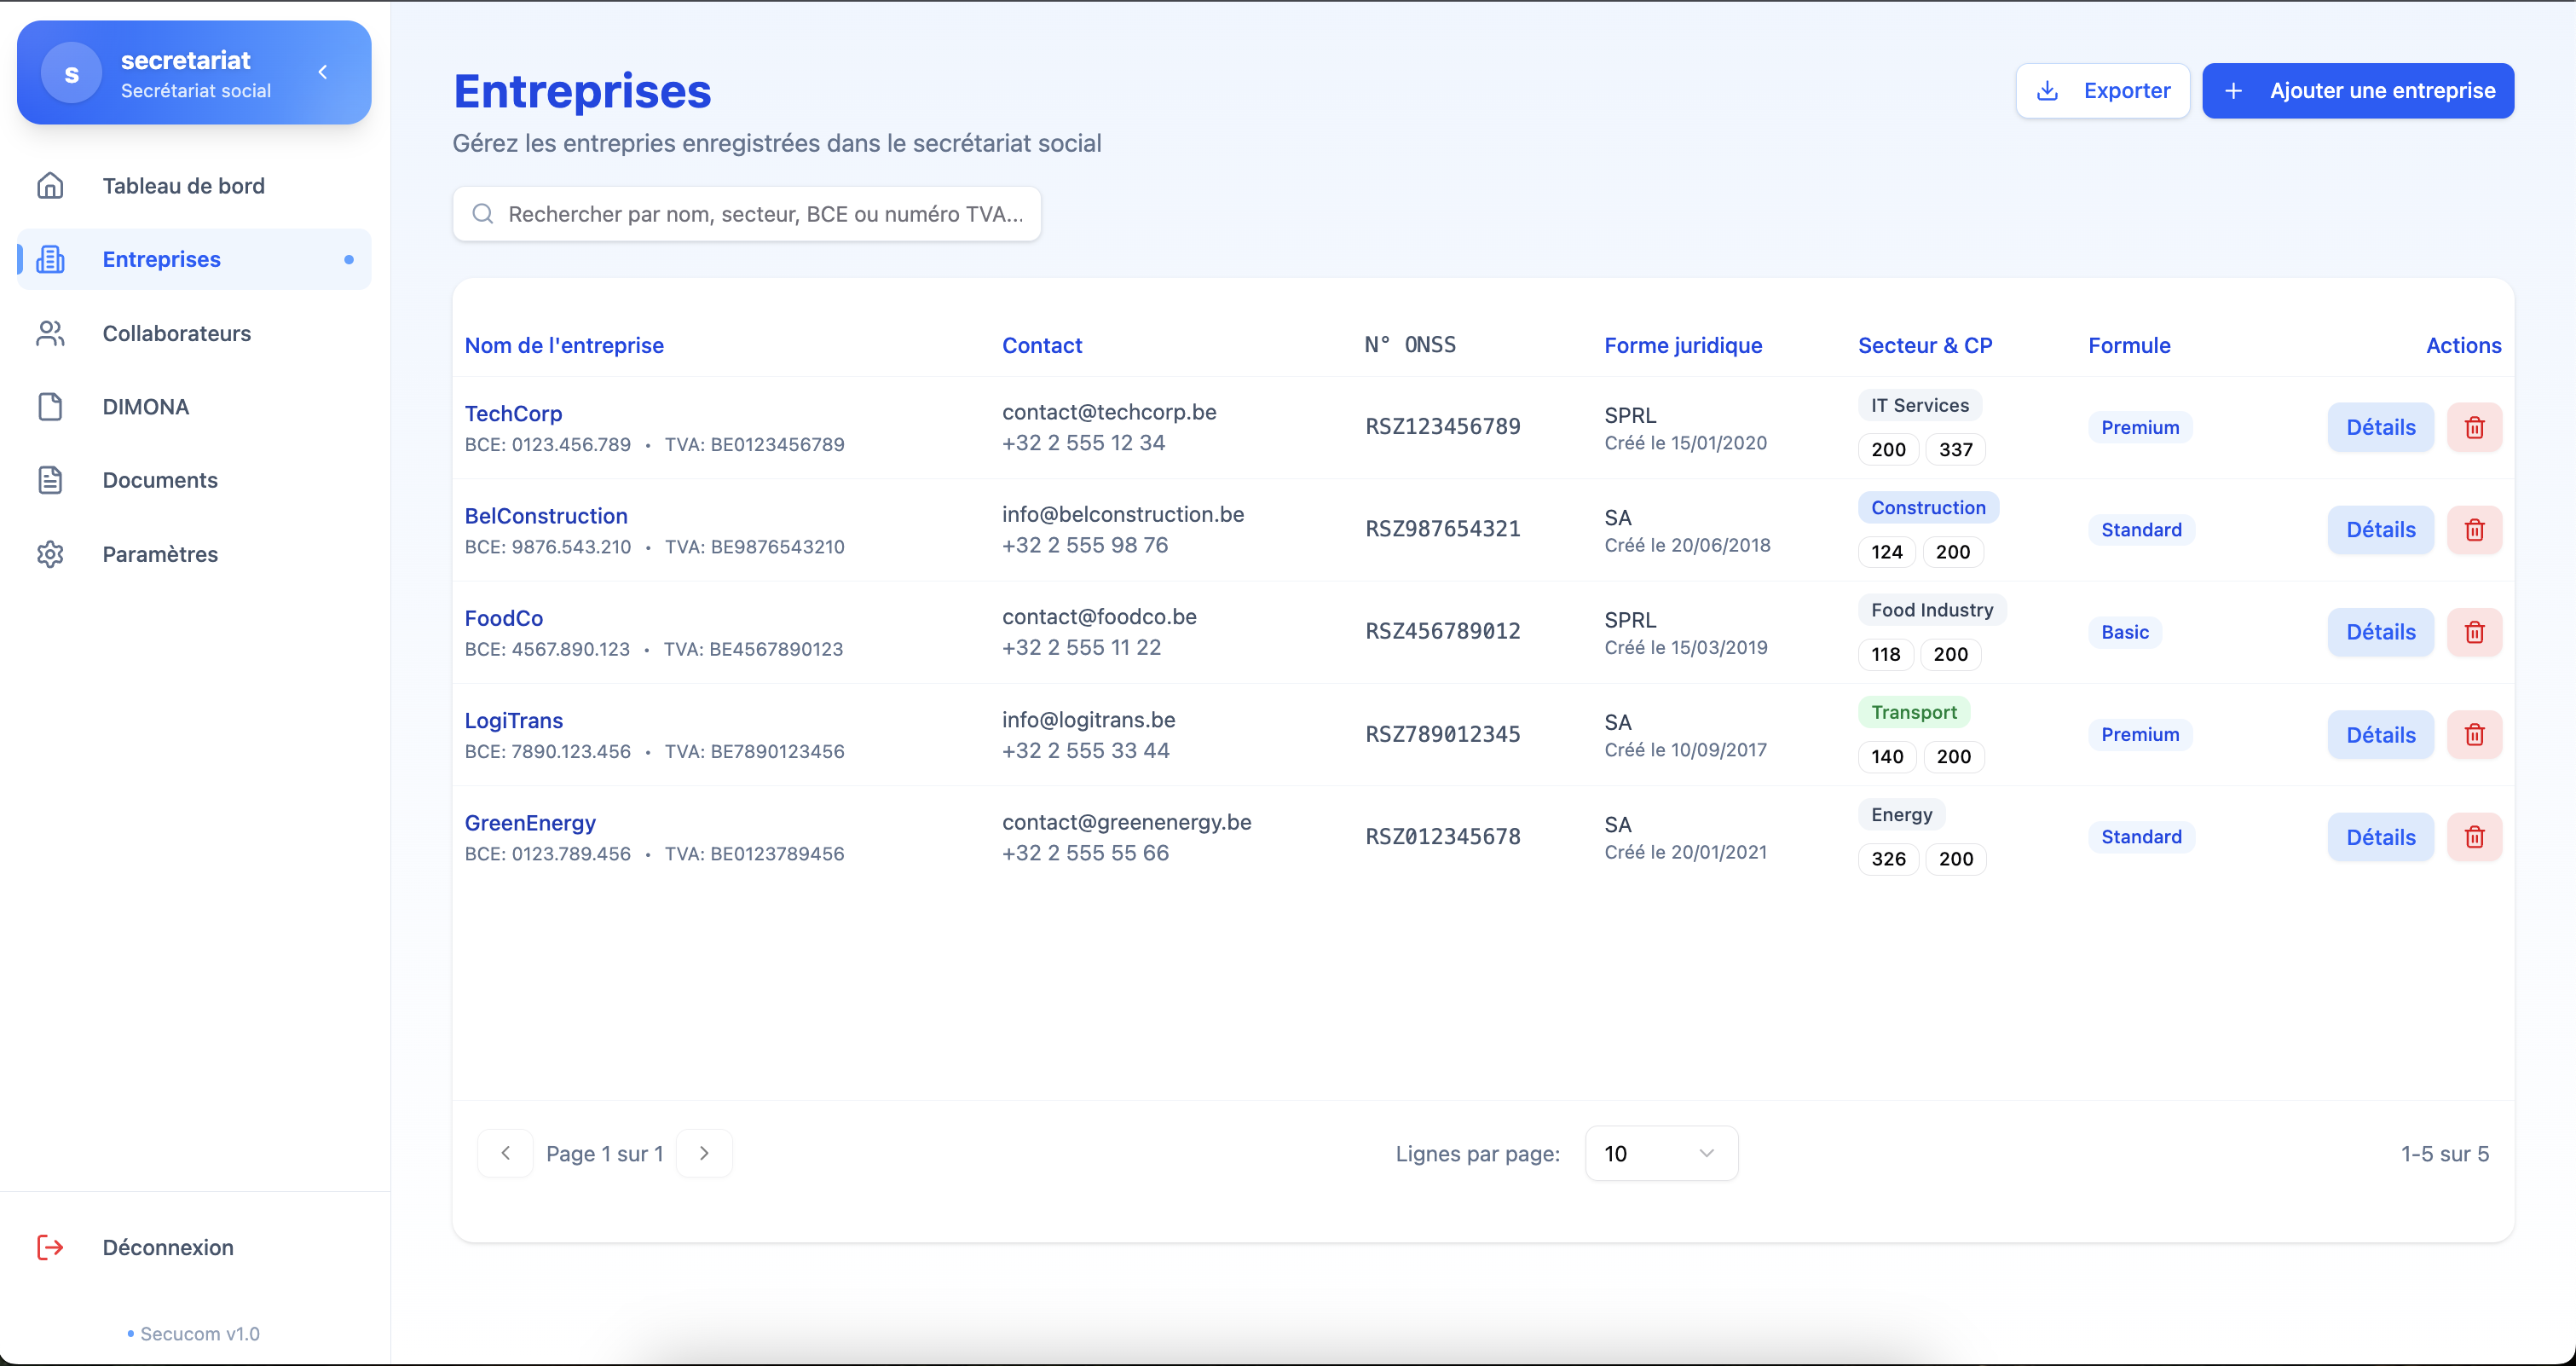
\includegraphics[width=1\textwidth]{SecuComPreviewCompanyList.png}
  \caption{Interface de gestion des entreprises dans SecuCom}
  \label{fig:companyManagementInterface}
\end{figure}

\subsubsection{Modèle de données}

Le modèle de données pour les entreprises est centré autour de l'entité \texttt{Company}, qui stocke toutes les informations nécessaires :

\vspace{0.5cm}

\begin{itemize}[leftmargin=*,label=\textcolor{darkgray}{$\bullet$},itemsep=0.3em]
  \item \textbf{Informations d'identification} : nom, numéro BCE, numéro ONSS, numéro TVA
  \item \textbf{Informations de contact} : téléphone, email, adresse
  \item \textbf{Informations bancaires} : IBAN
  \item \textbf{Informations légales} : forme juridique, secteur d'activité, commissions paritaires
  \item \textbf{Informations de collaboration} : date de début, formule souscrite, fréquence de déclaration
\end{itemize}

\vspace{0.5cm}

Cette entité est liée à d'autres entités importantes :
\begin{itemize}[leftmargin=*,label=\textcolor{darkgray}{$\bullet$},itemsep=0.3em]
  \item \texttt{CompanyContact} : Utilisateurs ayant accès aux données de l'entreprise
  \item \texttt{Collaborator} : Travailleurs de l'entreprise
  \item \texttt{Dimona} : Déclarations DIMONA associées à l'entreprise
\end{itemize}

\subsubsection{API REST}

L'API REST pour la gestion des entreprises est exposée par le \texttt{CompanyController}, qui offre les endpoints suivants :

\vspace{0.5cm}

\begin{tcolorbox}[
  title={\textbf{Endpoints de gestion des entreprises}},
  colback=blue!5!white,
  colframe=primarycolor,
  fonttitle=\bfseries,
  boxrule=0.5mm,
  arc=2mm,
  left=6mm,
  right=6mm,
  top=6mm,
  bottom=6mm
]
\begin{itemize}[leftmargin=*,label=\textcolor{darkgray}{$\bullet$},itemsep=0.3em]
  \item \texttt{POST /company} : Création d'une nouvelle entreprise
  \item \texttt{GET /company/\{id\}} : Récupération des détails d'une entreprise
  \item \texttt{GET /company} : Récupération de la liste des entreprises
  \item \texttt{PUT /company/\{id\}} : Mise à jour des informations d'une entreprise
  \item \texttt{DELETE /company/\{id\}} : Suppression d'une entreprise
  \item \texttt{GET /company/check/bce/\{bceNumber\}} : Vérification de l'existence d'un numéro BCE
  \item \texttt{GET /company/check/onss/\{onssNumber\}} : Vérification de l'existence d'un numéro ONSS
  \item \texttt{GET /company/check/vat/\{vatNumber\}} : Vérification de l'existence d'un numéro TVA
\end{itemize}
\end{tcolorbox}

\vspace{0.5cm}

\begin{note}
Ces endpoints sont sécurisés et accessibles uniquement aux utilisateurs autorisés (administrateurs et employés du secrétariat social).
\end{note}
\newpage

\subsubsection{Logique métier}

La logique métier pour la gestion des entreprises est implémentée dans le \texttt{CompanyService}, qui offre les fonctionnalités suivantes :

\vspace{0.5cm}

\begin{itemize}[leftmargin=*,label=\textcolor{darkgray}{$\bullet$},itemsep=0.3em]
  \item Validation des données d'entreprise (unicité des numéros BCE, ONSS et TVA)
  \item Création et mise à jour des entreprises avec gestion des relations
  \item Récupération des entreprises avec filtrage et pagination
  \item Suppression des entreprises avec gestion des dépendances
\end{itemize}

\vspace{0.5cm}

Le service implémente également des règles métier spécifiques, comme la vérification de la validité des numéros BCE et ONSS selon les formats belges.

\subsubsection{Gestion des contacts d'entreprise}

La gestion des contacts d'entreprise est une fonctionnalité complémentaire qui permet de définir quels utilisateurs ont accès aux données d'une entreprise. Elle est implémentée à travers le \texttt{CompanyContactService} et le \texttt{CompanyContactController}.

\vspace{0.5cm}

\begin{tcolorbox}[
  title={\textbf{Accès sécurisé par entreprise}},
  colback=blue!5!white,
  colframe=primarycolor,
  fonttitle=\bfseries,
  boxrule=0.5mm,
  arc=2mm,
  left=6mm,
  right=6mm,
  top=6mm,
  bottom=6mm
]
Les contacts d'entreprise sont des utilisateurs spécialisés (héritant de \texttt{User}) qui ont le rôle \texttt{ROLE\_COMPANY} et sont associés à une entreprise spécifique. Ils peuvent accéder uniquement aux données de leur propre entreprise, ce qui garantit une séparation stricte des données entre les différents clients du secrétariat social.
\end{tcolorbox}

\subsection{Gestion des collaborateurs}

La gestion des collaborateurs est une autre fonctionnalité clé de SecuCom, permettant de gérer les travailleurs des entreprises clientes (qu'ils soient employés, ouvriers, freelances, stagiaires ou étudiants). Cette fonctionnalité est particulièrement importante car elle sert de base pour les déclarations DIMONA.

\vspace{0.5cm}

\begin{figure}[H]
  \centering
  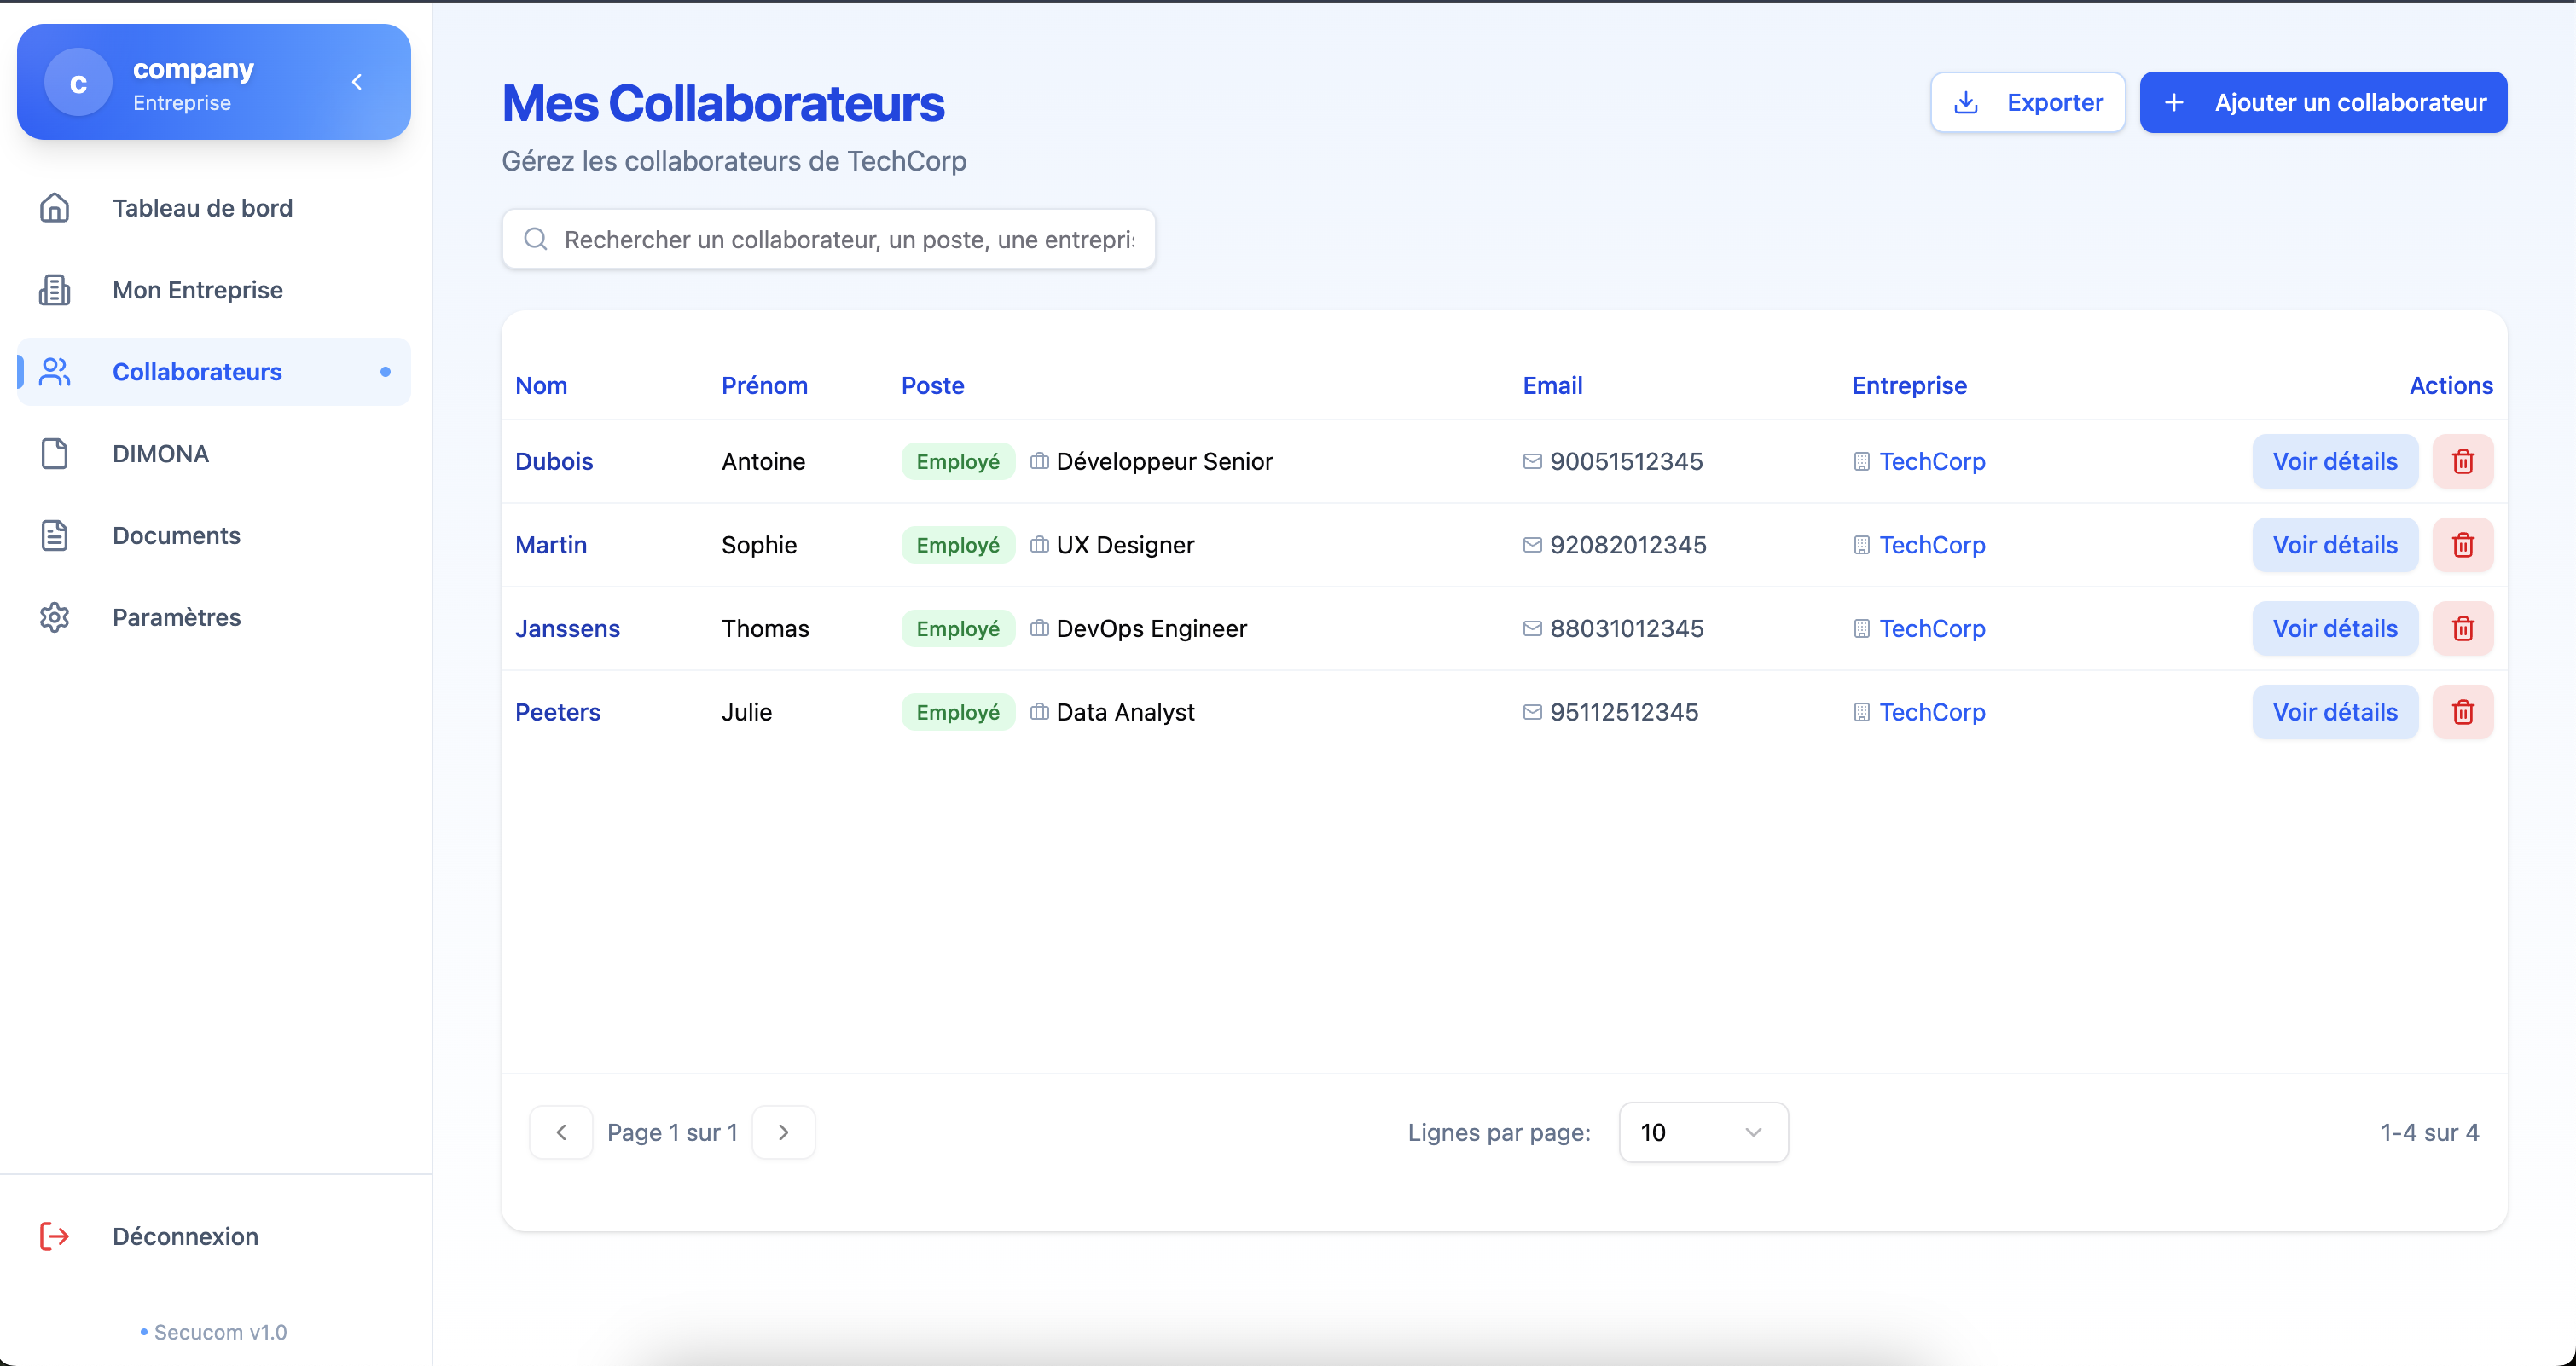
\includegraphics[width=1\textwidth]{SecuComPreviewCompanySpace.png}
  \caption{Interface de gestion des collaborateurs dans SecuCom}
  \label{fig:companyManagementInterface}
\end{figure}
\vspace{0.5cm}
\begin{figure}[H]
  \centering
  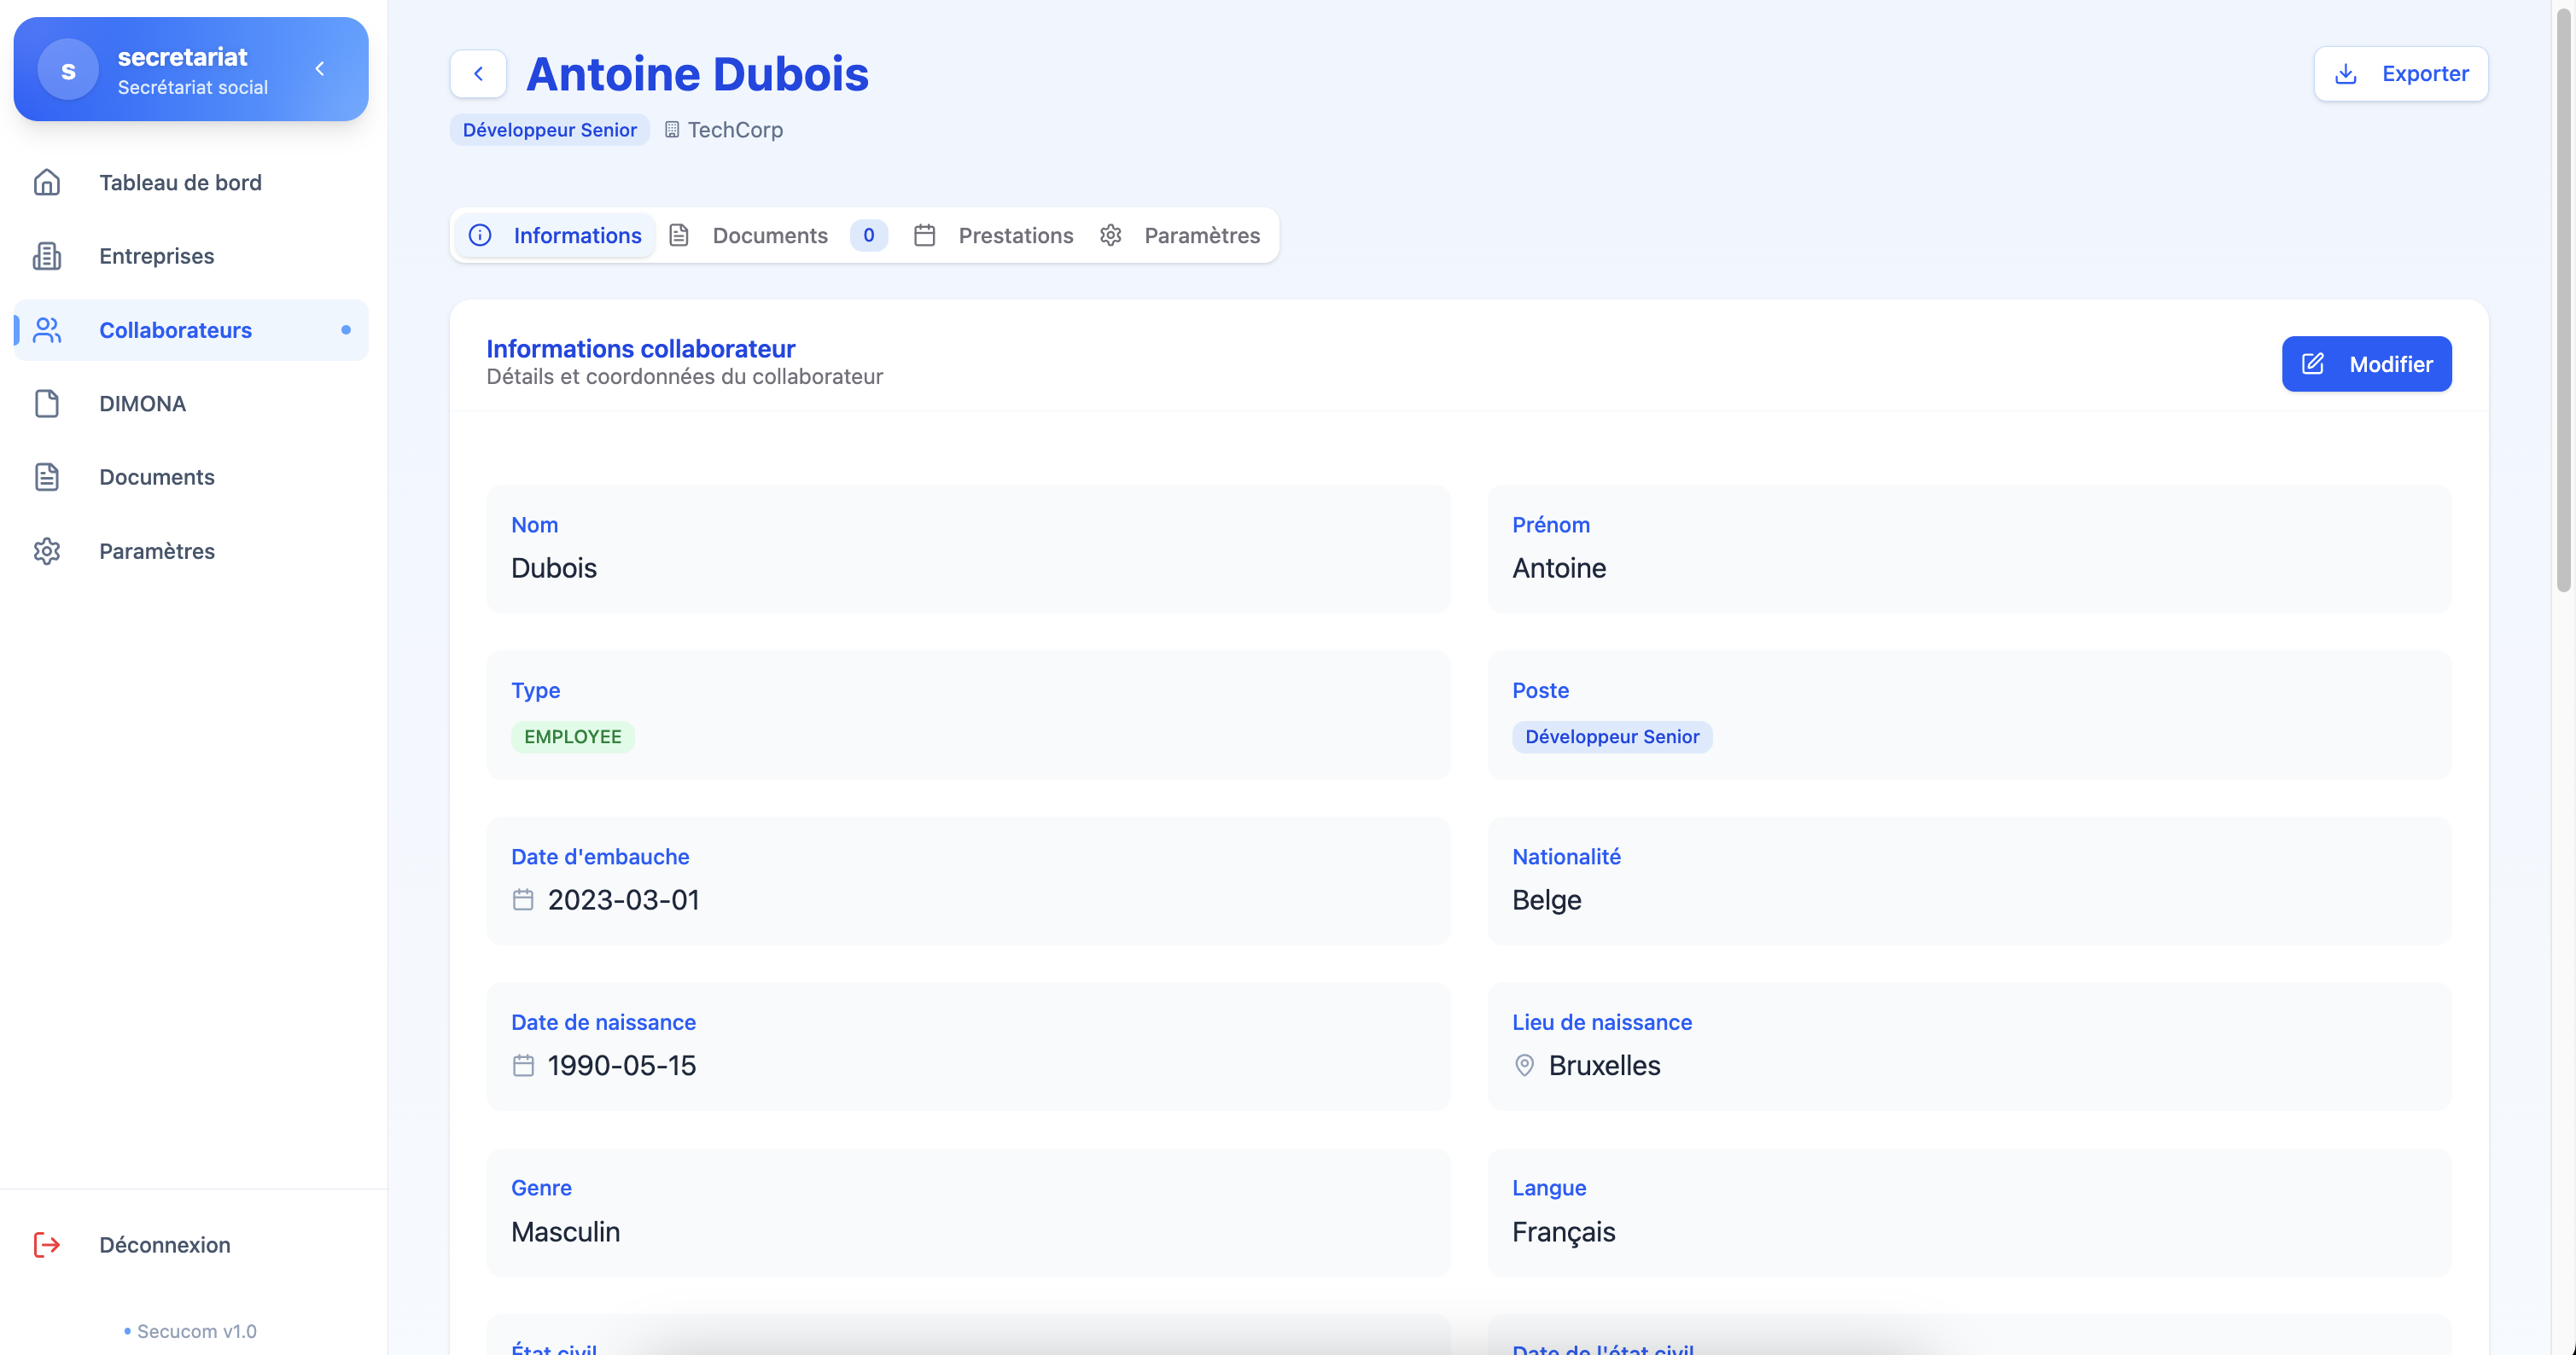
\includegraphics[width=1\textwidth]{SecuComPreviewCollaboratorInfos.png}
  \caption{Interface de gestion des collaborateurs dans SecuCom}
  \label{fig:companyManagementInterface}
\end{figure}

\subsubsection{Modèle de données}

Le modèle de données pour les collaborateurs est centré autour de l'entité \texttt{Collaborator}, qui stocke de nombreuses informations :

\vspace{0.5cm}

\begin{itemize}[leftmargin=*,label=\textcolor{darkgray}{$\bullet$},itemsep=0.3em]
  \item \textbf{Informations personnelles} : nom, prénom, nationalité, date de naissance, lieu de naissance, genre, langue, état civil
  \item \textbf{Informations d'identification} : numéro national (unique)
  \item \textbf{Informations professionnelles} : date d'entrée en service, fonction, type de contrat, régime de travail
  \item \textbf{Informations de rémunération} : salaire, avantages extra-légaux
  \item \textbf{Informations bancaires} : IBAN pour le versement du salaire
\end{itemize}

\vspace{0.5cm}

L'entité \texttt{Collaborator} utilise plusieurs types énumérés pour catégoriser les collaborateurs :
\begin{itemize}[leftmargin=*,label=\textcolor{darkgray}{$\bullet$},itemsep=0.3em]
  \item \texttt{CollaboratorType} : EMPLOYEE, WORKER, FREELANCE, INTERN, STUDENT
  \item \texttt{WorkDurationType} : FIXED, VARIABLE
  \item \texttt{Day} : MONDAY, TUESDAY, WEDNESDAY, THURSDAY, FRIDAY, SATURDAY, SUNDAY (pour les horaires)
\end{itemize}

\vspace{0.5cm}

\begin{note}
Elle utilise également des classes embarquées comme \texttt{Address} pour structurer les informations d'adresse, permettant une meilleure organisation des données et une réutilisation des structures communes.
\end{note}

\subsubsection{API REST}

L'API REST pour la gestion des collaborateurs est exposée par le \texttt{CollaboratorController}, qui offre les endpoints suivants :

\vspace{0.5cm}

\begin{tcolorbox}[
  title={\textbf{Endpoints de gestion des collaborateurs}},
  colback=blue!5!white,
  colframe=primarycolor,
  fonttitle=\bfseries,
  boxrule=0.5mm,
  arc=2mm,
  left=6mm,
  right=6mm,
  top=6mm,
  bottom=6mm
]
\begin{itemize}[leftmargin=*,label=\textcolor{darkgray}{$\bullet$},itemsep=0.3em]
  \item \texttt{POST /collaborators} : Création d'un nouveau collaborateur
  \item \texttt{GET /collaborators/\{id\}} : Récupération des détails d'un collaborateur
  \item \texttt{GET /collaborators} : Récupération de la liste des collaborateurs
  \item \texttt{GET /collaborators/company/\{companyId\}} : Récupération des collaborateurs d'une entreprise
  \item \texttt{PUT /collaborators/\{id\}} : Mise à jour des informations d'un collaborateur
  \item \texttt{DELETE /collaborators/\{id\}} : Suppression d'un collaborateur
\end{itemize}
\end{tcolorbox}

\vspace{0.5cm}

Ces endpoints sont sécurisés et accessibles aux utilisateurs autorisés, avec des restrictions basées sur les rôles et les associations d'entreprise.

\newpage

\subsubsection{Logique métier}

La logique métier pour la gestion des collaborateurs est implémentée dans le \texttt{CollaboratorService}, qui offre les fonctionnalités suivantes :

\vspace{0.5cm}

\begin{itemize}[leftmargin=*,label=\textcolor{darkgray}{$\bullet$},itemsep=0.3em]
  \item Validation des données de collaborateur (unicité du numéro national, validité des dates)
  \item Création et mise à jour des collaborateurs avec gestion des relations
  \item Récupération des collaborateurs avec filtrage par entreprise
  \item Suppression des collaborateurs avec gestion des dépendances (déclarations DIMONA)
\end{itemize}

\vspace{0.5cm}

Le service implémente également des règles métier spécifiques, comme la vérification de la validité du numéro national selon le format belge et la gestion des horaires de travail selon le type de durée de travail (fixe ou variable).

\subsubsection{Validation des données}

La validation des données de collaborateur est particulièrement importante en raison des exigences légales pour les déclarations DIMONA. Elle est implémentée à plusieurs niveaux :

\vspace{0.5cm}

\begin{tcolorbox}[
  title={\textbf{Approche multi-niveaux de validation}},
  colback=blue!5!white,
  colframe=primarycolor,
  fonttitle=\bfseries,
  boxrule=0.5mm,
  arc=2mm,
  left=6mm,
  right=6mm,
  top=6mm,
  bottom=6mm
]
\begin{itemize}[leftmargin=*,label=\textcolor{darkgray}{$\bullet$},itemsep=0.3em]
  \item \textbf{Niveau présentation} : Validation des DTOs avec les annotations Jakarta Validation (\texttt{@NotNull}, \texttt{@Size}, \texttt{@Pattern}, etc.)
  \item \textbf{Niveau service} : Validation métier dans le service (cohérence des dates, validité du numéro national)
  \item \textbf{Niveau persistance} : Contraintes de base de données (unicité du numéro national)
\end{itemize}

Cette approche garantit l'intégrité et la validité des données de collaborateur, réduisant ainsi les risques d'erreur lors des déclarations officielles auprès de l'ONSS.
\end{tcolorbox}

\subsection{Gestion des déclarations DIMONA}

La gestion des déclarations DIMONA est une fonctionnalité critique de SecuCom, permettant de suivre les déclarations d'emploi auprès de l'ONSS. Cette fonctionnalité est essentielle pour la conformité légale des entreprises clientes.

\vspace{0.5cm}

\begin{figure}[H]
  \centering
  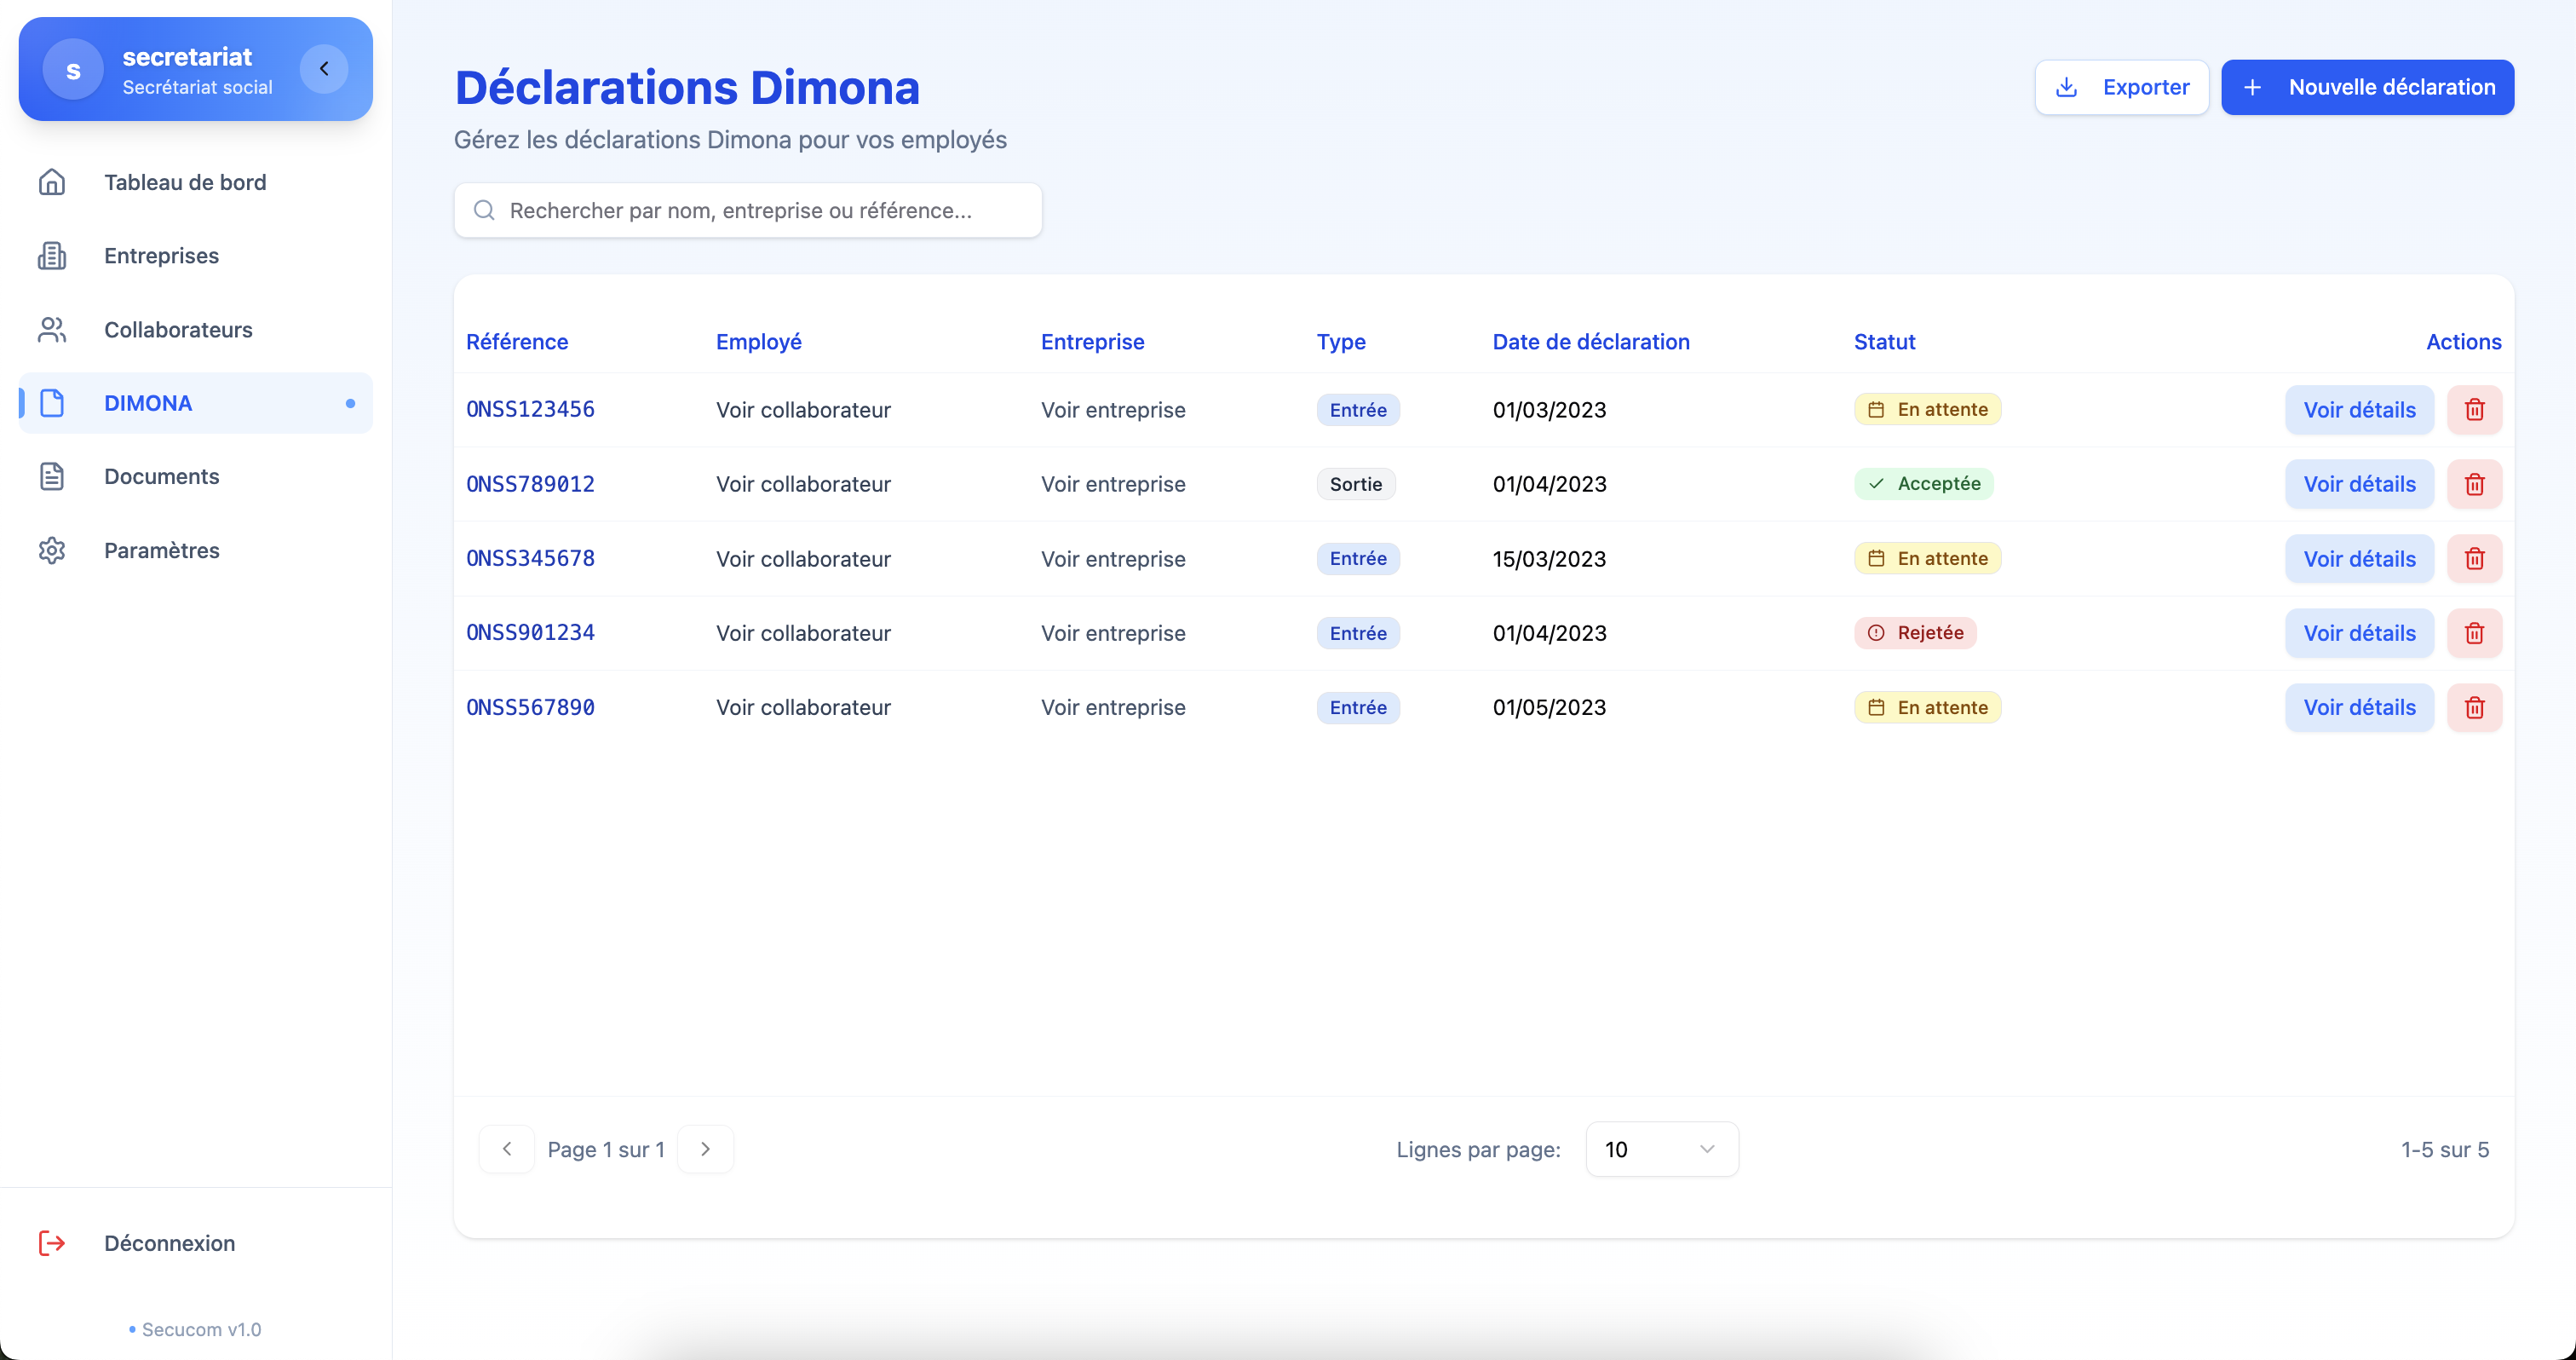
\includegraphics[width=1\textwidth]{SecuComPreviewDimona.png}
  \caption{Interface de gestion des dimonas dans SecuCom}
  \label{fig:companyInterface}
\end{figure}

\subsubsection{Modèle de données}

Le modèle de données pour les déclarations DIMONA est centré autour de l'entité \texttt{Dimona}, qui stocke les informations suivantes :

\vspace{0.5cm}

\begin{itemize}[leftmargin=*,label=\textcolor{darkgray}{$\bullet$},itemsep=0.3em]
  \item \textbf{Type de déclaration} : entrée en service, sortie de service
  \item \textbf{Dates} : dates d'entrée et de sortie
  \item \textbf{Raison de sortie} : si applicable
  \item \textbf{Statut} : 
  \item \textbf{Référence ONSS} : attribuée par l'ONSS après acceptation
  \item \textbf{Message d'erreur} : en cas de rejet
\end{itemize}

\vspace{0.5cm}

L'entité \texttt{Dimona} est liée à deux autres entités importantes :
\begin{itemize}[leftmargin=*,label=\textcolor{darkgray}{$\bullet$},itemsep=0.3em]
  \item \texttt{Collaborator} : Le travailleur concerné par la déclaration
  \item \texttt{Company} : L'entreprise employeuse
\end{itemize}

\vspace{0.5cm}

\begin{note}
Cette double association permet de retrouver facilement les déclarations par collaborateur ou par entreprise, facilitant ainsi les recherches et le reporting.
\end{note}

\subsubsection{API REST}

L'API REST pour la gestion des déclarations DIMONA est exposée par le \texttt{DimonaController}, qui offre les endpoints suivants :

\vspace{0.5cm}

\begin{tcolorbox}[
  title={\textbf{Endpoints de gestion des déclarations DIMONA}},
  colback=blue!5!white,
  colframe=primarycolor,
  fonttitle=\bfseries,
  boxrule=0.5mm,
  arc=2mm,
  left=6mm,
  right=6mm,
  top=6mm,
  bottom=6mm
]
\begin{itemize}[leftmargin=*,label=\textcolor{darkgray}{$\bullet$},itemsep=0.3em]
  \item \texttt{POST /dimona} : Création d'une nouvelle déclaration DIMONA
  \item \texttt{GET /dimona/\{id\}} : Récupération des détails d'une déclaration
  \item \texttt{GET /dimona} : Récupération de la liste des déclarations
  \item \texttt{GET /dimona/collaborator/\{collaboratorId\}} : Récupération des déclarations d'un collaborateur
  \item \texttt{GET /dimona/company/\{companyId\}} : Récupération des déclarations d'une entreprise
  \item \texttt{DELETE /dimona/\{id\}} : Suppression d'une déclaration
\end{itemize}
\end{tcolorbox}

\vspace{0.5cm}

Ces endpoints sont sécurisés et accessibles aux utilisateurs autorisés, avec des restrictions basées sur les rôles et les associations d'entreprise.

\subsubsection{Logique métier}

La logique métier pour la gestion des déclarations DIMONA est implémentée dans le \texttt{DimonaService}, qui offre les fonctionnalités suivantes :

\vspace{0.5cm}

\begin{itemize}[leftmargin=*,label=\textcolor{darkgray}{$\bullet$},itemsep=0.3em]
  \item Validation des données de déclaration (cohérence des dates, existence du collaborateur et de l'entreprise)
  \item Création des déclarations avec initialisation du statut
  \item Mise à jour du statut des déclarations après traitement par l'ONSS
  \item Récupération des déclarations avec filtrage par collaborateur ou entreprise
\end{itemize}

\vspace{0.5cm}

Le service implémente également des règles métier spécifiques, comme la vérification de la cohérence entre les dates d'entrée et de sortie, et la validation des types de déclaration selon le contexte.

\subsubsection{Processus de déclaration}

Le processus de déclaration DIMONA dans SecuCom est semi-automatisé :

\vspace{0.5cm}

\begin{tcolorbox}[
  title={\textbf{Flux de traitement d'une déclaration DIMONA}},
  colback=blue!5!white,
  colframe=primarycolor,
  fonttitle=\bfseries,
  boxrule=0.5mm,
  arc=2mm,
  left=6mm,
  right=6mm,
  top=6mm,
  bottom=6mm
]
\begin{enumerate}[itemsep=0.3em]
  \item Un utilisateur (contact d'entreprise ou employé du secrétariat) crée une demande de déclaration DIMONA dans le système.
  \item Le système valide les données et crée une entrée avec le statut "en attente".
  \item Un employé du secrétariat social traite la demande en soumettant manuellement la déclaration sur le site officiel de l'ONSS.
  \item Après traitement par l'ONSS, l'employé met à jour le statut et la référence ONSS dans le système.
  \item Le système notifie le contact d'entreprise du résultat de la déclaration.
\end{enumerate}
\end{tcolorbox}

\vspace{0.5cm}

\begin{note}
Cette approche semi-automatisée permet un contrôle humain sur les déclarations tout en bénéficiant de la validation et du suivi automatisés offerts par le système. Elle répond directement au besoin exprimé par Sodabel d'avoir un système de suivi des déclarations DIMONA.
\end{note}

\newpage
\section{Sécurité et authentification}

La sécurité est un aspect fondamental de SecuCom, étant donné la nature sensible des données traitées. L'application implémente un système robuste d'authentification et d'autorisation basé sur les tokens JWT (JSON Web Tokens).

\vspace{0.5cm}

\subsection{Authentification basée sur JWT}

L'authentification dans SecuCom est implémentée en utilisant les tokens JWT, qui offrent plusieurs avantages :
\begin{itemize}[leftmargin=*,label=\textcolor{darkgray}{$\bullet$},itemsep=0.3em]
  \item \textbf{Authentification sans état} (stateless), facilitant la scalabilité
  \item \textbf{Transmission sécurisée} des informations d'identité
  \item \textbf{Expiration automatique} des sessions
  \item \textbf{Possibilité de révocation} des tokens
\end{itemize}

\vspace{0.5cm}

\begin{tcolorbox}[
  title={\textbf{Processus d'authentification JWT}},
  colback=blue!5!white,
  colframe=primarycolor,
  fonttitle=\bfseries,
  boxrule=0.5mm,
  arc=2mm,
  left=6mm,
  right=6mm,
  top=6mm,
  bottom=6mm
]
\begin{enumerate}[itemsep=0.3em]
  \item L'utilisateur soumet ses identifiants (nom d'utilisateur/email et mot de passe) via l'endpoint \texttt{/auth/login}.
  \item Le système vérifie les identifiants et, s'ils sont valides, génère deux tokens :
    \begin{itemize}[leftmargin=*,label=\textcolor{darkgray}{$\bullet$},itemsep=0.3em]
      \item Un token d'accès (access token) de courte durée pour l'authentification
      \item Un token de rafraîchissement (refresh token) de longue durée pour obtenir de nouveaux tokens d'accès
    \end{itemize}
  \item Le token d'accès est renvoyé dans la réponse JSON, tandis que le token de rafraîchissement est stocké dans un cookie HTTP-only sécurisé.
  \item Pour les requêtes ultérieures, le client inclut le token d'accès dans l'en-tête \texttt{Authorization}.
  \item Lorsque le token d'accès expire, le client peut obtenir un nouveau token en utilisant le token de rafraîchissement via l'endpoint \texttt{/auth/refresh}.
\end{enumerate}
\end{tcolorbox}

\vspace{0.5cm}

Cette implémentation est réalisée à travers plusieurs classes :

\begin{itemize}[leftmargin=*,label=\textcolor{darkgray}{$\bullet$},itemsep=0.3em]
  \item \texttt{JwtUtils} : Génère et valide les tokens JWT
  \item \texttt{JwtAuthenticationFilter} : Intercepte les requêtes et extrait les tokens JWT
  \item \texttt{AuthController} : Expose les endpoints d'authentification
  \item \texttt{AuthService} : Implémente la logique d'authentification
  \item \texttt{UserDetailsServiceImpl} : Charge les détails utilisateur pour Spring Security
\end{itemize}

\subsection{Gestion des rôles et autorisations}

SecuCom implémente un système de contrôle d'accès basé sur les rôles (RBAC) en utilisant Spring Security. Trois rôles principaux sont définis :

\vspace{0.5cm}

\begin{table}[H]
\centering
\begin{tabular}{|l|p{10cm}|}
\hline
\textbf{Rôle} & \textbf{Description} \\
\hline
\texttt{ROLE\_ADMIN} & Administrateurs du système avec accès complet à toutes les fonctionnalités \\
\hline
\texttt{ROLE\_SECRETARIAT} & Employés du secrétariat social avec accès à toutes les entreprises clientes et leurs données \\
\hline
\texttt{ROLE\_COMPANY} & Contacts d'entreprise avec accès limité aux données de leur propre entreprise \\
\hline
\end{tabular}
\caption{Rôles utilisateurs dans SecuCom}
\end{table}

\vspace{0.5cm}

Ces rôles sont utilisés à plusieurs niveaux pour sécuriser l'application :

\begin{itemize}[leftmargin=*,label=\textcolor{darkgray}{$\bullet$},itemsep=0.3em]
  \item \textbf{Niveau URL} : Certains endpoints sont restreints à des rôles spécifiques via la configuration de Spring Security dans \texttt{SecurityConfig}.
  \item \textbf{Niveau méthode} : Des annotations comme \texttt{@PreAuthorize} sont utilisées pour sécuriser des methodes spécifiques dans les contrôleurs et services.
  \item \textbf{Niveau données} : Des filtres sont appliqués dans les services pour limiter l'accès aux données selon le rôle et l'association d'entreprise de l'utilisateur.
\end{itemize}

\vspace{0.5cm}

\begin{note}
Par exemple, un utilisateur avec le rôle \texttt{ROLE\_COMPANY} ne peut accéder qu'aux données de sa propre entreprise, tandis qu'un utilisateur avec le rôle \texttt{ROLE\_SECRETARIAT} peut accéder aux données de toutes les entreprises.
\end{note}

\subsection{Sécurisation des communications}

Toutes les communications entre le client et le serveur sont sécurisées via HTTPS/TLS, assurant la confidentialité et l'intégrité des données en transit. La configuration CORS (Cross-Origin Resource Sharing) est également mise en place pour contrôler quels domaines peuvent accéder aux ressources de l'API.

\subsection{Gestion des exceptions de sécurité}

SecuCom implémente une gestion centralisée des exceptions via \texttt{GlobalExceptionHandler}, qui intercepte les exceptions liées à la sécurité et renvoie des réponses appropriées sans exposer de détails sensibles.

\vspace{0.5cm}

\begin{tcolorbox}[
  title={\textbf{Avantages de la gestion centralisée des exceptions}},
  colback=blue!5!white,
  colframe=primarycolor,
  fonttitle=\bfseries,
  boxrule=0.5mm,
  arc=2mm,
  left=6mm,
  right=6mm,
  top=6mm,
  bottom=6mm
]
Cette approche garantit que les erreurs de sécurité sont traitées de manière cohérente et sécurisée, sans révéler d'informations qui pourraient être exploitées par des attaquants. Elle permet également de standardiser les formats de réponse d'erreur à travers toute l'application.
\end{tcolorbox}

\subsection{Protection des mots de passe}

Les mots de passe des utilisateurs sont protégés à l'aide de l'algorithme de hachage BCrypt, qui intègre automatiquement un sel (salt) unique pour chaque mot de passe, rendant les attaques par dictionnaire et par table arc-en-ciel (rainbow table) inefficaces.

\vspace{0.5cm}

\begin{note}
Lors de l'authentification, le mot de passe fourni est haché et comparé au hachage stocké, sans jamais manipuler le mot de passe en clair, conformément aux bonnes pratiques de sécurité.
\end{note}

\subsection{Audit et traçabilité}

SecuCom intègre des mécanismes d'audit pour tracer les actions importantes des utilisateurs. Les entités principales incluent des champs d'audit comme \texttt{createdAt}, \texttt{updatedAt} et \texttt{lastLogin}, qui sont automatiquement mis à jour grâce à l'annotation \texttt{@EntityListeners(AuditingEntityListener.class)}.

\vspace{0.5cm}

Cette traçabilité permet non seulement de suivre l'historique des modifications, mais aussi de détecter d'éventuelles activités suspectes et de faciliter les investigations en cas d'incident de sécurité.

\vspace{1cm}

\begin{tcolorbox}[
  title={\textbf{Sécurité transversale}},
  colback=blue!5!white,
  colframe=primarycolor,
  fonttitle=\bfseries,
  boxrule=0.5mm,
  arc=2mm,
  left=6mm,
  right=6mm,
  top=6mm,
  bottom=6mm
]
En résumé, la sécurité de SecuCom est implémentée de manière transversale à travers toutes les couches de l'application, assurant la protection des données sensibles et la conformité avec les exigences légales en matière de protection des données. Cette approche holistique de la sécurité est essentielle pour une application manipulant des données personnelles et professionnelles sensibles.
\end{tcolorbox}


% Aspects financiers
\chapter{Aspects financiers}

Cette section présente une estimation simplifiée des coûts et bénéfices de SecuCom dans le cadre de ce TFE.

\section{Coûts de développement}

\subsection{Coûts des ressources humaines}

Dans le cadre d'un projet étudiant, les coûts sont estimés à des tarifs académiques :

\begin{table}[h]
\centering
\begin{tabular}{|l|c|c|c|}
\hline
\textbf{Rôle} & \textbf{Tarif journalier} & \textbf{Jours} & \textbf{Coût total} \\
\hline
Développeur backend & 150€ & 20 & 3.000€ \\
Développeur frontend & 150€ & 15 & 2.250€ \\
Analyste & 150€ & 5 & 750€ \\
Tests & 150€ & 5 & 750€ \\
\hline
\textbf{Total} & & \textbf{45} & \textbf{6.750€} \\
\hline
\end{tabular}
\caption{Coûts des ressources humaines}
\end{table}

\subsection{Coûts d'infrastructure}

\begin{table}[h]
\centering
\begin{tabular}{|l|c|}
\hline
\textbf{Élément} & \textbf{Coût annuel} \\
\hline
Hébergement cloud & 360€ \\
Base de données & 240€ \\
Nom de domaine et SSL & 50€ \\
\hline
\textbf{Total} & \textbf{650€} \\
\hline
\end{tabular}
\caption{Coûts d'infrastructure}
\end{table}

\subsection{Récapitulatif}

\begin{table}[h]
\centering
\begin{tabular}{|l|c|}
\hline
\textbf{Catégorie} & \textbf{Coût} \\
\hline
Développement initial & 6.750€ \\
Infrastructure (première année) & 650€ \\
\hline
\textbf{Total investissement initial} & \textbf{7.400€} \\
\hline
\end{tabular}
\caption{Récapitulatif des coûts}
\end{table}

\section{Bénéfices attendus}

\subsection{Gains de productivité}

\begin{table}[h]
\centering
\begin{tabular}{|l|c|c|c|}
\hline
\textbf{Processus} & \textbf{Temps avant} & \textbf{Temps après} & \textbf{Gain} \\
\hline
Création d'entreprise & 45 min & 15 min & 67\% \\
Ajout de collaborateur & 30 min & 10 min & 67\% \\
Déclaration DIMONA & 20 min & 5 min & 75\% \\
Recherche d'informations & 15 min & 2 min & 87\% \\
\hline
\end{tabular}
\caption{Gains de productivité estimés}
\end{table}

Pour Sodabel (50 entreprises, 5 collaborateurs/entreprise, 200 DIMONA/an), ces gains représentent environ 500 heures économisées par an.

\subsection{Réduction des erreurs}

\begin{table}[h]
\centering
\begin{tabular}{|l|c|c|}
\hline
\textbf{Type d'erreur} & \textbf{Taux actuel} & \textbf{Taux attendu} \\
\hline
Erreurs de saisie & 5\% & < 1\% \\
DIMONA rejetées & 8\% & < 2\% \\
Informations manquantes & 12\% & < 3\% \\
\hline
\end{tabular}
\caption{Réduction des erreurs attendue}
\end{table}

\subsection{Bénéfices qualitatifs}

\begin{itemize}
  \item Image professionnelle améliorée
  \item Satisfaction client accrue
  \item Meilleure traçabilité des opérations
  \item Réduction du stress pour les employés
  \item Capacité à gérer plus de clients sans augmenter les ressources
\end{itemize}

\subsection{Retour sur investissement}

En valorisant les gains de temps (500h × 20€ = 10.000€/an) et la réduction des erreurs (environ 2.000€/an), le retour sur investissement initial serait atteint en moins d'un an.

\begin{table}[h]
\centering
\begin{tabular}{|l|c|c|c|}
\hline
\textbf{Année} & \textbf{Investissement} & \textbf{Bénéfices} & \textbf{Bilan} \\
\hline
Année 0 & 7.400€ & 0€ & -7.400€ \\
Année 1 & 650€ & 12.000€ & +3.950€ \\
\hline
\end{tabular}
\caption{Projection du retour sur investissement}
\end{table}

SecuCom représente donc un investissement raisonnable avec un retour rapide pour Sodabel, tout en offrant une base solide pour des développements futurs.


% Conclusion
\chapter*{Conclusion}
\addcontentsline{toc}{chapter}{Conclusion}
\markboth{Conclusion}{}

Cette section présente une synthèse du projet SecuCom, en abordant les difficultés rencontrées, le bilan global et les perspectives d'évolution future.

\section*{Défis rencontrées}
\addcontentsline{toc}{section}{Difficultés rencontrées}
\markright{Difficultés rencontrées}

Le développement de SecuCom a présenté plusieurs défis techniques et conceptuels qui ont nécessité des solutions innovantes :

\begin{itemize}[leftmargin=*,label=\textcolor{darkgray}{$\bullet$},itemsep=0.3em]
  \item \textbf{Complexité du domaine métier} : La compréhension approfondie des processus d'un secrétariat social belge, notamment les spécificités des déclarations DIMONA et les exigences légales associées, a représenté un défi initial important. Cette complexité a nécessité de nombreux échanges avec Sodabel pour s'assurer que l'application réponde précisément aux besoins réels.

  \item \textbf{Compréhension des besoins du client} : L'un des défis majeurs a été de bien cerner les attentes et besoins réels de Sodabel, au-delà des demandes initiales parfois trop ambitieuses. Ce processus a nécessité une communication constante et une capacité d'analyse pour distinguer les besoins essentiels des fonctionnalités secondaires.

  \item \textbf{Savoir dire non et gérer le périmètre} : Apprendre à refuser certaines demandes lorsqu'elles dépassaient le cadre réalisable du projet a constitué une difficulté importante. Cette compétence s'est avérée cruciale pour maintenir le projet dans des limites réalistes en termes de temps et de ressources disponibles.

  \item \textbf{Sécurisation des données sensibles} : La manipulation de données personnelles et professionnelles confidentielles a imposé la mise en place d'une architecture de sécurité robuste. L'implémentation du système d'authentification JWT et la gestion fine des autorisations basées sur les rôles ont demandé une attention particulière pour garantir la confidentialité et l'intégrité des données.

  \item \textbf{Séparation des espaces utilisateurs} : La création d'espaces distincts pour le secrétariat social et les entreprises clientes, tout en maintenant une cohérence dans l'expérience utilisateur, a constitué un défi architectural. Il a fallu concevoir un système où les données sont strictement cloisonnées tout en permettant une navigation fluide.

  \item \textbf{Équilibre entre ambition et faisabilité} : Le projet initial comportait un nombre important de fonctionnalités qui ont dû être réduites pour s'adapter aux contraintes de temps et de ressources. Cette situation a imposé un exercice constant de priorisation et de recentrage sur l'essentiel, tout en concevant une architecture suffisamment modulaire pour permettre des extensions futures.
\end{itemize}

\section*{Bilan}
\addcontentsline{toc}{section}{Bilan}
\markright{Bilan}

\textbf{Le développement de SecuCom peut être considéré comme un succès dans la mesure où les objectifs initiaux ont été atteints :}

\begin{itemize}[leftmargin=*,label=\textcolor{darkgray}{$\bullet$},itemsep=0.3em]
  \item \textbf{Réponse aux besoins identifiés} : L'application répond directement aux problématiques concrètes identifiées chez Sodabel, notamment la digitalisation des processus manuels, la centralisation des communications et la réduction des risques d'erreurs. Les gains de productivité estimés (environ 67\% pour la création d'entreprise, environ 75\% pour les déclarations DIMONA selon les estimations) démontrent la pertinence de la solution.

  \item \textbf{Architecture technique solide} : L'utilisation de technologies modernes et éprouvées (Spring Boot, ReactJS, JWT) a permis de construire une base technique robuste, sécurisée et évolutive. La séparation claire des responsabilités entre les différentes couches de l'application facilite sa maintenance et son extension future.

  \item \textbf{Approche modulaire réussie} : Malgré la réduction du périmètre initial, l'architecture modulaire adoptée permet d'envisager sereinement l'ajout de nouvelles fonctionnalités sans remettre en question les fondations du système. Cette approche s'est avérée être un choix judicieux face aux contraintes du projet.

  \item \textbf{Positionnement stratégique} : Face aux solutions existantes comme EasyPay et Liantis, SecuCom se distingue par son approche ciblée et minimaliste, répondant spécifiquement aux besoins des petits secrétariats sociaux. Cette spécialisation constitue un avantage concurrentiel dans un marché dominé par des solutions généralistes souvent surdimensionnées.

  \item \textbf{Apprentissage de la priorisation} : Le processus de développement a permis d'acquérir une compétence essentielle : la capacité à identifier et prioriser les fonctionnalités vraiment essentielles, plutôt que de se disperser dans une multitude de fonctionnalités secondaires. Cette leçon constitue un acquis précieux pour les projets futurs.
\end{itemize}

Ce projet a également permis de démontrer qu'une approche ciblée, privilégiant la qualité et la pertinence des fonctionnalités plutôt que leur quantité, peut apporter une valeur significative dans un domaine aussi complexe que celui des secrétariats sociaux.

\section*{Améliorations futures}
\addcontentsline{toc}{section}{Améliorations futures}
\markright{Améliorations futures}

SecuCom a été conçu dès le départ comme une plateforme évolutive, destinée à s'enrichir progressivement de nouvelles fonctionnalités. Plusieurs axes d'amélioration ont été identifiés pour les développements futurs, notamment ceux qui avaient été envisagés initialement mais qui ont dû être reportés pour respecter les contraintes du projet :

\newpage
\subsection*{Demandes de services}
\addcontentsline{toc}{subsection}{Demandes de services}

L'implémentation d'un système de demandes de services permettrait aux entreprises clientes de solliciter directement via la plateforme différents types de prestations auprès du secrétariat social :

\begin{itemize}[leftmargin=*,label=\textcolor{darkgray}{$\bullet$},itemsep=0.3em]
  \item Module de création de demandes avec catégorisation (conseil juridique, modification administrative, attestation spécifique, etc.)
  \item Système de suivi en temps réel de l'état d'avancement des demandes
  \item Notifications automatiques informant les clients des mises à jour
  \item Historique des demandes permettant de consulter les échanges passés
  \item Tableau de bord pour le secrétariat social facilitant la gestion et la priorisation des demandes
\end{itemize}

Cette fonctionnalité remplacerait avantageusement les échanges actuels par email et WhatsApp, centralisant toutes les communications dans un espace structuré et traçable.

\subsection*{Gestion et génération de documents}
\addcontentsline{toc}{subsection}{Gestion et génération de documents}

Le développement d'un système complet de gestion documentaire constituerait une amélioration majeure :

\begin{itemize}[leftmargin=*,label=\textcolor{darkgray}{$\bullet$},itemsep=0.3em]
  \item Génération automatique de documents officiels (contrats de travail, C4, fiches de paie) à partir des données du système
  \item Modèles de documents personnalisables adaptés aux besoins spécifiques de chaque entreprise
  \item Système de signature électronique pour faciliter la validation des documents
  \item Archivage sécurisé avec classification et recherche avancée
  \item Gestion des versions permettant de suivre l'évolution des documents
\end{itemize}

Cette fonctionnalité réduirait considérablement le temps consacré à la création manuelle de documents et minimiserait les risques d'erreurs dans leur production.

\subsection*{Facturation automatique}
\addcontentsline{toc}{subsection}{Facturation automatique}

L'intégration d'un système de facturation automatique pour les services et documents fournis via la plateforme apporterait une valeur ajoutée significative :

\begin{itemize}[leftmargin=*,label=\textcolor{darkgray}{$\bullet$},itemsep=0.3em]
  \item Génération automatique de factures basée sur les services rendus et les documents produits
  \item Paramétrage flexible des tarifs selon le type de client et de service
  \item Suivi des paiements avec relances automatiques
  \item Tableau de bord financier offrant une vue d'ensemble des revenus
  \item Intégration avec des solutions comptables pour faciliter la réconciliation
\end{itemize}

Cette fonctionnalité permettrait non seulement d'optimiser le processus de facturation, mais aussi d'améliorer le suivi financier des prestations du secrétariat social.

\subsection*{Autres améliorations potentielles}
\addcontentsline{toc}{subsection}{Autres améliorations potentielles}

Au-delà des trois axes principaux mentionnés, d'autres améliorations pourraient enrichir SecuCom :

\begin{itemize}[leftmargin=*,label=\textcolor{darkgray}{$\bullet$},itemsep=0.3em]
  \item Intégration directe avec l'ONSS pour automatiser complètement les déclarations DIMONA
  \item Tableau de bord analytique offrant des insights sur l'activité des entreprises clientes
  \item Système de chat intégré pour les communications en temps réel entre le secrétariat et ses clients
  \item Implémentation du protocole HTTPS pour sécuriser les communications entre le client et le serveur, essentielle dans l'objectif d'un déploiement en production serein et conforme aux standards de sécurité actuels
\end{itemize}

\section*{Conclusion générale}
\addcontentsline{toc}{section}{Conclusion générale}
\markright{Conclusion générale}

SecuCom représente bien plus qu'un simple projet académique ; il constitue une réponse concrète et viable à des problématiques réelles rencontrées par les secrétariats sociaux de petite taille. En privilégiant une approche ciblée et minimaliste, le projet a su apporter une valeur ajoutée immédiate tout en posant les fondations d'une évolution future.\\

Les fonctionnalités actuellement implémentées (gestion des entreprises, des collaborateurs et des déclarations DIMONA) répondent aux besoins les plus critiques identifiés lors de l'analyse initiale. Les améliorations futures envisagées, notamment les demandes de services, la gestion documentaire et la facturation automatique, s'inscrivent dans une vision cohérente d'évolution progressive de la plateforme.\\

L'une des leçons les plus importantes tirées de ce projet est l'importance de la modularité et de la priorisation. Face à des ambitions initiales trop vastes, la capacité à recentrer le projet sur les fonctionnalités essentielles tout en concevant une architecture permettant des extensions futures s'est avérée déterminante pour atteindre les objectifs fixés.\\

En définitive, SecuCom illustre comment une solution informatique bien conçue, même avec un périmètre fonctionnel volontairement limité, peut transformer des processus métier traditionnels, apportant efficacité, sécurité et satisfaction tant aux prestataires de services qu'à leurs clients. La véritable réussite du projet réside peut-être moins dans l'étendue des fonctionnalités développées que dans la solidité des fondations posées pour l'avenir.\\


% Bibliographie
\begin{thebibliography}{99}

\bibitem{sodabel}
Sodabel. (2023).
\textit{Secrétariat social pour entreprises et indépendants}.

\bibitem{dimona}
Office National de Sécurité Sociale. (2023).
\textit{DIMONA - Déclaration Immédiate/Onmiddellijke Aangifte}.
Récupéré de \url{https://www.socialsecurity.be/site_fr/employer/applics/dimona/index.htm}

\bibitem{onss}
Office National de Sécurité Sociale. (2023).
\textit{Portail de la sécurité sociale}.
Récupéré de \url{https://www.socialsecurity.be}

\bibitem{spf-emploi}
Service Public Fédéral Emploi, Travail et Concertation sociale. (2023).
\textit{Guide de la réglementation sociale pour les entreprises}.
Récupéré de \url{https://emploi.belgique.be/fr/themes/contrats-de-travail}

\bibitem{spf-emploi-dimona}
Service Public Fédéral Emploi. (2023).
\textit{Obligations liées à la DIMONA}.
Récupéré de \url{https://emploi.belgique.be/fr/themes/contrats-de-travail/declaration-dimona}

\bibitem{easypay}
EasyPay Group. (2023).
\textit{Solutions pour secrétariats sociaux}.
Récupéré de \url{https://www.easypay-group.com/fr_BE/}

\bibitem{liantis}
Liantis. (2023).
\textit{Services de secrétariat social}.
Récupéré de \url{https://www.liantis.be/fr}

\bibitem{spring-boot}
Spring. (2023).
\textit{Spring Boot}.
Récupéré de \url{https://spring.io/projects/spring-boot}

\bibitem{spring-security}
Spring. (2023).
\textit{Spring Security}.
Récupéré de \url{https://spring.io/projects/spring-security}

\bibitem{spring-data}
Spring. (2023).
\textit{Spring Data JPA}.
Récupéré de \url{https://spring.io/projects/spring-data-jpa}

\bibitem{hibernate}
Hibernate. (2023).
\textit{Hibernate ORM}.
Récupéré de \url{https://hibernate.org/orm/}

\bibitem{react}
React. (2023).
\textit{Une bibliothèque JavaScript pour créer des interfaces utilisateurs}.
Récupéré de \url{https://fr.reactjs.org/}

\bibitem{shadcn-ui}
shadcn. (2023).
\textit{shadcn/ui - Composants d'interface utilisateur réutilisables}.
Récupéré de \url{https://ui.shadcn.com/}

\bibitem{tailwind}
Tailwind CSS. (2023).
\textit{Framework CSS utilitaire pour créer rapidement des designs personnalisés}.
Récupéré de \url{https://tailwindcss.com/}

\bibitem{jwt}
JWT.io. (2023).
\textit{Introduction aux JSON Web Tokens}.
Récupéré de \url{https://jwt.io/introduction}

\bibitem{bce}
Banque-Carrefour des Entreprises. (2023).
\textit{Portail de la BCE}.
Récupéré de \url{https://economie.fgov.be/fr/themes/entreprises/banque-carrefour-des}

\bibitem{rgpd}
Autorité de protection des données. (2023).
\textit{RGPD pour les entreprises}.
Récupéré de \url{https://www.autoriteprotectiondonnees.be/professionnel}

\bibitem{pappers-sodabel}
Pappers.be. (2023).
\textit{Informations sur Sodabel SRL}.
Récupéré de \url{https://www.pappers.be/fr/company/sodabel-0751606280}

\end{thebibliography}


% Glossaire
\chapter*{Glossaire}
\addcontentsline{toc}{chapter}{Glossaire}

\begin{description}[leftmargin=2cm, style=nextline]

\item[API (Application Programming Interface)] Interface de programmation qui permet à différentes applications de communiquer entre elles. Dans SecuCom, une API RESTful est utilisée pour la communication entre le frontend et le backend.

\item[BCE (Banque-Carrefour des Entreprises)] Registre contenant toutes les données d'identification des entreprises en Belgique. Chaque entreprise y reçoit un numéro d'identification unique.

\item[DIMONA (Déclaration Immédiate/Onmiddellijke Aangifte)] Système belge de déclaration obligatoire de tout engagement ou fin de relation de travail auprès de l'Office National de Sécurité Sociale (ONSS).

\item[DTO (Data Transfer Object)] Objet utilisé pour transporter des données entre différentes couches d'une application. Dans SecuCom, les DTOs sont utilisés pour la communication entre le frontend et le backend.

\item[Hibernate] Framework de mapping objet-relationnel (ORM) pour Java qui facilite la persistance des objets Java dans une base de données relationnelle.

\item[IBAN (International Bank Account Number)] Format international de numéro de compte bancaire utilisé pour identifier un compte bancaire de manière unique.

\item[JPA (Java Persistence API)] Spécification Java qui décrit la gestion des données relationnelles dans les applications Java. Dans SecuCom, Spring Data JPA est utilisé pour l'accès aux données.

\item[JWT (JSON Web Token)] Standard ouvert qui définit un format compact et autonome pour la transmission sécurisée d'informations entre parties sous forme d'objet JSON. Dans SecuCom, JWT est utilisé pour l'authentification et l'autorisation.

\item[Microservices] Style d'architecture qui structure une application comme un ensemble de services faiblement couplés. Bien que SecuCom ne soit pas actuellement basé sur une architecture microservices, cette approche pourrait être envisagée pour des évolutions futures.

\item[ONSS (Office National de Sécurité Sociale)] Organisme public belge chargé de la perception et de la gestion des cotisations sociales des employeurs et des travailleurs.

\item[ORM (Object-Relational Mapping)] Technique de programmation qui convertit les données entre des systèmes de types incompatibles dans des bases de données relationnelles et des langages de programmation orientés objet. Hibernate est l'ORM utilisé dans SecuCom.

\item[ReactJS] Bibliothèque JavaScript open-source utilisée pour construire des interfaces utilisateur, particulièrement pour les applications à page unique. ReactJS est utilisé pour le développement du frontend de SecuCom.

\item[RGPD (Règlement Général sur la Protection des Données)] Règlement de l'Union européenne qui constitue le texte de référence en matière de protection des données à caractère personnel. SecuCom est conçu pour être conforme au RGPD.

\item[Secrétariat social] En Belgique, organisme privé agréé qui aide les employeurs à accomplir leurs obligations administratives et sociales liées à l'emploi de personnel.

\item[Spring Boot] Framework Java qui simplifie le développement d'applications Java en fournissant une configuration par défaut pour les projets Spring. Spring Boot est utilisé pour le développement du backend de SecuCom.

\item[Spring Security] Module du framework Spring qui fournit des services d'authentification et d'autorisation pour les applications Java. Spring Security est utilisé dans SecuCom pour la gestion de la sécurité.

\item[SRL (Société à Responsabilité Limitée)] Forme juridique d'entreprise en Belgique où la responsabilité des associés est limitée à leurs apports. Sodabel est une SRL.

\item[TypeScript] Langage de programmation open-source développé par Microsoft qui ajoute le typage statique optionnel à JavaScript. TypeScript est utilisé dans le frontend de SecuCom pour améliorer la maintenabilité et la détection d'erreurs.

\item[UML (Unified Modeling Language)] Langage de modélisation graphique utilisé en génie logiciel pour visualiser, spécifier, construire et documenter les artefacts d'un système. Plusieurs diagrammes UML sont utilisés dans ce document pour illustrer l'architecture de SecuCom.

\end{description}


% Annexes
\appendix
\chapter{Annexes}
\section{Diagrammes UML complémentaires}
Cette annexe présente des diagrammes UML supplémentaires qui n'ont pas été inclus dans le corps principal du document mais qui apportent des précisions sur l'architecture et le fonctionnement de SecuCom.

\section{Code source des composants principaux}
Cette annexe présente les extraits de code source les plus significatifs du projet, accompagnés d'explications détaillées sur leur fonctionnement et leur rôle dans l'architecture globale.

\section{Manuel d'utilisation}
Cette annexe fournit un guide d'utilisation simplifié de la plateforme SecuCom, destiné aux utilisateurs finaux (employés du secrétariat social et contacts des entreprises clientes).

\end{document}
